
% Тип документа
\documentclass[a4paper,12pt]{extarticle}

% Шрифты, кодировки, символьные таблицы, переносы
\usepackage{cmap}
\usepackage[T2A]{fontenc}
\usepackage[utf8x]{inputenc}
\usepackage[russian]{babel}

% Это пакет -- хитрый пакет, он нужен но не нужен
\usepackage[mode=buildnew]{standalone}

\usepackage
	{
		% Дополнения Американского математического общества (AMS)
		amssymb,
		amsfonts,
		amsmath,
		amsthm,
		physics,
		% misccorr,
		% 
		% Графики и рисунки
		wrapfig,
		graphicx,
		subcaption,
		float,
		tikz,
		tikz-3dplot,
		caption,
		csvsimple,
		color,
		booktabs,
		pgfplots,
		pgfplotstable,
		geometry,
		% 
		% Таблицы, списки
		makecell,
		multirow,
		indentfirst,
		%
		% Интегралы и прочие обозначения
		ulem,
		esint,
		esdiff,
		% 
		% Колонтитулы
		fancyhdr,
	}  

\usepackage{xcolor}
\usepackage{hyperref}

 % Цвета для гиперссылок
\definecolor{linkcolor}{HTML}{000000} % цвет ссылок
\definecolor{urlcolor}{HTML}{799B03} % цвет гиперссылок
 
\hypersetup{pdfstartview=FitH,  linkcolor=linkcolor,urlcolor=urlcolor, colorlinks=true}
% Обводка текста в TikZ
\usepackage[outline]{contour}

% Увеличенный межстрочный интервал, французские пробелы
\linespread{1.3} 
\frenchspacing 

 
\usetikzlibrary
	{
		decorations.pathreplacing,
		decorations.pathmorphing,
		patterns,
		calc,
		scopes,
		arrows,
		fadings,
		through,
		shapes.misc,
		arrows.meta,
		3d,
		quotes,
		angles,
		babel
	}


\tikzset{
	force/.style=	{
		>=latex,
		draw=blue,
		fill=blue,
				 	}, 
	%				 	
	axis/.style=	{
		densely dashed,
		blue,
		line width=1pt,
		font=\small,
					},
	%
	th/.style=	{
		line width=1pt},
	%
	acceleration/.style={
		>=open triangle 60,
		draw=magenta,
		fill=magenta,
					},
	%
	inforce/.style=	{
		force,
		double equal sign distance=2pt,
					},
	%
	interface/.style={
		pattern = north east lines, 
		draw    = none, 
		pattern color=gray!60,
					},
	cross/.style=	{
		cross out, 
		draw=black, 
		minimum size=2*(#1-\pgflinewidth), 
		inner sep=0pt, outer sep=0pt,
					},
	%
	cargo/.style=	{
		rectangle, 
		fill=black!70, 
		inner sep=2.5mm,
					},
	%
	caption/.style= {
		midway,
		fill=white!20, 
		opacity=0.9
					},
	%
	}

\newenvironment{tikzpict}
    {
	    \begin{figure}[htbp]
		\centering
		\begin{tikzpicture}
    }
    { 
		\end{tikzpicture}
		% \caption{caption}
		% \label{fig:label}
		\end{figure}
    }


\newcommand{\vbLabel}[3]{\draw ($(#1,#2)+(0,5pt)$) -- ($(#1,#2)-(0,5pt)$) node[below]{#3}}
\newcommand{\vaLabel}[3]{\draw ($(#1,#2)+(0,5pt)$) node[above]{#3} -- ($(#1,#2)-(0,5pt)$) }

\newcommand{\hrLabel}[3]{\draw ($(#1,#2)+(5pt,0)$) -- ($(#1,#2)-(5pt,0)$) node[right, xshift=1em]{#3}}
\newcommand{\hlLabel}[3]{\draw ($(#1,#2)+(5pt,0)$) node[left, xshift=-1em]{#3} -- ($(#1,#2)-(5pt,0)$) }



\newcommand\zi{^{\,*}_i}
\newcommand\sumn{\sum_{i=1}^{N}}

\tikzset{
	coordsys/.style={scale=1.8,x={(1.1cm,-0cm)},y={(0.5cm,1cm)}, z={(0cm,0.8cm)}},
	coordsys/.style={scale=1.5,x={(0cm,0cm)},y={(1cm,0cm)}, z={(0cm,1cm)}}, 
	coordsys/.style={scale=1.5,x={(1cm,0cm)},y={(0cm,1cm)}, z={(0cm,0cm)}}, 
}

\usepgfplotslibrary{units}


% Draw line annotation
% Input:
%   #1 Line offset (optional)
%   #2 Line angle
%   #3 Line length
%   #5 Line label
% Example:
%   \lineann[1]{30}{2}{$L_1$}

\newcommand{\lineann}[4][0.5]{%
    \begin{scope}[rotate=#2, blue,inner sep=2pt, ]
        \draw[dashed, blue!40] (0,0) -- +(0,#1)
            node [coordinate, near end] (a) {};
        \draw[dashed, blue!40] (#3,0) -- +(0,#1)
            node [coordinate, near end] (b) {};
        \draw[|<->|] (a) -- node[fill=white, scale=0.8] {#4} (b);
    \end{scope}
}

\newcommand{\lineannn}[4][0.5]{%
    \begin{scope}[rotate=#2, blue,inner sep=2pt, ]
        \draw[dashed, blue!40] (0,0) -- +(0,#1)
            node [coordinate, near end] (a) {};
        \draw[dashed, blue!40] (#3,0) -- +(0,#1)
            node [coordinate, near end] (b) {};
        % \draw[color=white, color=blue] (a) -- node[fill=white, scale=0.8] {#4} (b);
        \draw[->|] (a)++(-0.3,0) -- (a);
        \draw[->|] (b)++(0.3,0) coordinate (xx) -- (b);
        \draw (xx) node[fill=white, scale=0.8, right] {#4};
    \end{scope}
}

% Круговая стрелка относительно центра (дуга из центра)
\tikzset{
  pics/carc/.style args={#1:#2:#3}{
    code={
      \draw[pic actions] (#1:#3) arc(#1:#2:#3);
    }
  },
  dash/.style={
  	dash pattern=on 5mm off 5mm
  }
}

% Среднее <#1>
\newcommand{\mean}[1]{\langle#1\rangle}

\pgfplotsset{
    % most recent feature set of pgfplots
    compat=newest,
}

% const прямым шрифтом
\newcommand\ct[1]{\text{\rmfamily\upshape #1}}
\newcommand*{\const}{\ct{const}}


\usepackage[europeanresistors,americaninductors]{circuitikz}

% Style to select only points from #1 to #2 (inclusive)
\pgfplotsset{select/.style 2 args={
    x filter/.code={
        \ifnum\coordindex<#1\def\pgfmathresult{}\fi
        \ifnum\coordindex>#2\def\pgfmathresult{}\fi
    }
}}


\usepackage{array}
\usepackage{pstool}


%%%%%%%%%%%%%%%%%%%%%%%%%%%%%%%%%%%%%%%%%%%%%%%%%
\makeatletter
\newif\if@gather@prefix 
\preto\place@tag@gather{% 
  \if@gather@prefix\iftagsleft@ 
    \kern-\gdisplaywidth@ 
    \rlap{\gather@prefix}% 
    \kern\gdisplaywidth@ 
  \fi\fi 
} 
\appto\place@tag@gather{% 
  \if@gather@prefix\iftagsleft@\else 
    \kern-\displaywidth 
    \rlap{\gather@prefix}% 
    \kern\displaywidth 
  \fi\fi 
  \global\@gather@prefixfalse 
} 
\preto\place@tag{% 
  \if@gather@prefix\iftagsleft@ 
    \kern-\gdisplaywidth@ 
    \rlap{\gather@prefix}% 
    \kern\displaywidth@ 
  \fi\fi 
} 
\appto\place@tag{% 
  \if@gather@prefix\iftagsleft@\else 
    \kern-\displaywidth 
    \rlap{\gather@prefix}% 
    \kern\displaywidth 
  \fi\fi 
  \global\@gather@prefixfalse 
} 
\newcommand*{\beforetext}[1]{% 
  \ifmeasuring@\else
  \gdef\gather@prefix{#1}% 
  \global\@gather@prefixtrue 
  \fi
} 
\makeatother
%%%%%%%%%%%%%%%%%%%%%%%%%%%%%%%%%%%%%%%%%%%%%%%%%

\geometry		
	{
		left			=	2cm,
		right 			=	2cm,
		top 			=	3cm,
		bottom 			=	3cm,
		bindingoffset	=	0cm
	}

%%%%%%%%%%%%%%%%%%%%%%%%%%%%%%%%%%%%%%%%%%%%%%%%%%%%%%%%%%%%%%%%%%%%%%%%%%%%%%%



	%применим колонтитул к стилю страницы
\pagestyle{fancy} 
	%очистим "шапку" страницы
\fancyhead{} 
	%слева сверху на четных и справа на нечетных
\fancyhead[R]{\labauthors} 
	%справа сверху на четных и слева на нечетных
\fancyhead[L]{Отчёт по лабораторной работе №\labnumber} 
	%очистим "подвал" страницы
\fancyfoot{} 
	% номер страницы в нижнем колинтуле в центре
\fancyfoot[C]{\thepage} 

%%%%%%%%%%%%%%%%%%%%%%%%%%%%%%%%%%%%%%%%%%%%%%%%%%%%%%%%%%%%%%%%%%%%%%%%%%%%%%%

\renewcommand{\contentsname}{Оглавление}

\usepackage{tocloft}
% \renewcommand{\cftpartleader}{\cftdotfill{\cftdotsep}} % for parts
% \renewcommand{\cftsectiondotsep}{\cftdotsep}% Chapters should use dots in ToC
\renewcommand{\cftsecleader}{\cftdotfill{\cftdotsep}}
%\renewcommand{\cftsecleader}{\cftdotfill{\cftdotsep}} % for sections, if you really want! (It is default in report and book class (So you may not need it).
% ---------
% \newcommand{\cftchapaftersnum}{.}%
% \usepackage{titlesec}
% \titlelabel{\thetitle.\quad}
\usepackage{secdot}
\sectiondot{subsection}

\begin{document}

\def\labauthors{Войтович Д.А., Понур К.А.}
\def\labgroup{430}
\def\labnumber{2}
\def\labtheme{Фазовая плоскость лампового генератора}
\begin{titlepage}

\begin{center}

{\small\textsc{Нижегородский государственный университет имени Н.\,И. Лобачевского}}
\vskip 1pt \hrule \vskip 3pt
{\small\textsc{Радиофизический факультет}}

\vfill

{\Large Отчет по лабораторной работе №\labnumber\vskip 12pt\bfseries \labtheme}
	
\end{center}

\vfill
	
\begin{flushright}
	{Выполнили студенты \labgroup\ группы\\ \labauthors}%\vskip 12pt Принял:\\ Менсов С.\,Н.}
\end{flushright}
	
\vfill
	
\begin{center}
	Нижний Новгород, \the\year
\end{center}

\end{titlepage}



\tableofcontents
\newpage




\section{Теоретическая часть}
\subsubsection*{Цель работы} Изучение различных режимов возбуждения лампового генератора и установление зависимости амплитуды и частоты автоколебаний от параметров системы.

Аппаратом теоретического рассмотрения является метод Ван-дер-Поля. Полученные с его помощью результаты сравниваются с результатами экспериментального исследования фазовой плоскости изучаемой системы. 
\subsection{ Метод Ван-дер-Поля}
Слабонелинейные квазиконсервативные системы могут совершать периодические движения с постоянной амплитудой, определяемой свойствами системы. Таким периодическим движениям на фазовой плоскости соответствуют изолированные замкнутые фазовые траектории, называемые {\itshapeпредельными циклами}.

Предельный цикл будет устойчивым, если все фазовые траектории, начинающиеся в малой окрестности предельного цикла, будут асимптотически приближаться при $t\to\infty$.

Динамические системы, а фазовом портрете которых имеется, по крайней мере, один устойчивый предельный цикл, называются автоколебательными. 

Будем считать, что система описывается уравнением вида 
\begin{equation}
\label{eq:1}
\ddot{x}+x=\mu f(x,\dot{x}),
\end{equation}
где  $f(x,\dot{x})$ - нелинейная ограниченная функция 

~$\mu$ - малый безразмерный параметр.

Нас интересуют периодические решения. Метод Ван-дер-Поля позволяет задачу отыскания периодических решений уравнения (\ref{eq:1}) свести к несравненно более простой - задаче нахождения состояний равновесия так называемых укороченных уравнений. Перейдем к их составлению.

При $\mu=0$ уравнение (\ref{eq:1}) описывает обычный гармонический осциллятор, и его решение можно записать в виде:

$$x=A\cos(t+\varphi)=A\cos\theta,$$
\begin{equation}
\label{eq:2}
\dot{x}=y=-A\sin(t+\varphi)=-A\sin\theta,
\end{equation}
где А и $\varphi$ - произвольные постоянные, имеющие физический смысл амплитуды и фазы колебаний. 

\newpage
Решение можно представить и в комплексной форме в виде: 
\begin{gather}
\label{eq:3}
x=ze^{jt}+z^*e^{-jt},\\\notag
\dot{x}=y=j(ze^{jt}-z^*e^{-jt}),
\end{gather}
где z и $z^*$ - произвольные постоянные, являющиеся комплексной и комплексно сопряженной амплитудами.  

Решение вида  (\ref{eq:3}) легко сводится к виду  (\ref{eq:2}), если положить $$z=\rho e^{j\varphi}, z^*=\rho e^{-j\varphi}$$

В результате получим:

\begin{center}
$x=\rho(e^{j(t+\varphi)}+e^{-j(t+\varphi)})=2\rho \cos(t+\varphi)$,

$\dot{x}=y=j\rho(e^{j(t+\varphi)}-e^{-j(t+\varphi)})=2\rho \sin(t+\varphi)$.
\end{center}
Следовательно, 
\begin{gather}
\label{eq:4}
|z|=|z^*|=\rho=\frac{A}{2},\\\notag
argz=-argz^*=\varphi.
\end{gather}

При $\mu \ne 0$, но сколь угодно малом, решение уравнения (\ref{eq:1})  не должно существенно отличаться от решения для линейного осциллятора, поэтому будем его искать в виде (\ref{eq:2}) , считая теперь А и $\varphi$ не постоянными величинами, а некоторыми неизвестными функциями времени:

\begin{center}
$\dot{x}=\dot{A} \cos\theta-A(1+\dot \varphi)\sin\theta=-A\sin\theta$, $\theta=t+\varphi$
\end{center}

Откуда следует $$\dot{A}\cos\theta-A\dot \varphi \sin\theta=0.$$

Подставляя решение  (\ref{eq:2}) в уравнение  (\ref{eq:1}), будем иметь $$\dot{A}\sin\theta+a\dot \varphi \cos\theta=-\mu f(A\cos\theta;-A\sin\theta).$$
Разрешая два последних уравнения относительно $\dot{A}$ и $\dot{\varphi}$, получаем систему
\begin{gather}
\label{eq:5}
\dot{A}=-\mu f(A\cos\theta;-A\sin\theta)\sin\theta,\\\notag
A\dot{\varphi}=-\mu f(A\cos\theta;-A\sin\theta) \cos\theta.
\end{gather}
адекватную уравнению (\ref{eq:1}), но записанную в других переменных, называемых переменными Ван-дер-Поля. Полученная система не является более простой по сравнению с уравнением (\ref{eq:1}). Однако, если учесть, что $\mu \ll 1$, то из нее можно получить приближенную, значительно более простую систему.

Правая часть системы  (\ref{eq:5}) является периодической функцией явно входящего времени $\theta=t+\varphi$ и зависит от А и $\varphi$. Поскольку  А и $\varphi$ являются медленно меняющимися функциями времени, то можно их считать постоянными на периоде быстрых осцилляций. Воспользуемся этим и, проинтегрировав уравнения, определим средние значения за период $T=2\pi$. Заметим, что интегрирование можно проводить не по времени, а по $\theta=t+\varphi$. В результате получим систему
\begin{gather}
\label{eq:6}
\frac{dA}{dt}=-\frac{\mu}{2\pi}\int\limits_\theta^{\theta+2\pi} f(A\cos\theta;-A\sin\theta)\sin\theta d\theta,\\\notag
\frac{d\varphi}{dt}=-\frac{\mu}{2\pi A}\int\limits_\theta^{\theta+2\pi} f(A\cos\theta;-A\sin\theta)\cos\theta d\theta.
\end{gather}

Запишем ее в виде
   
\begin{equation}
\label{eq:7}
\frac{dA}{dt}=\mu \Phi(A),~\frac{d\varphi}{dt}=\mu \phi(A),
\end{equation}
где $\Phi(A)$ и $\phi(A)$ - средние за период значения периодических функций, зависящие только от А: $$-f(A\cos\theta;-A\sin\theta)\sin\theta,~~f(-\frac{1}{A} \cos\theta;-A\sin\theta)\cos\theta.$$

Полученные уравнения  (\ref{eq:7}) и называются системой укороченных или усредненных уравнений. Эта система определяет амплитуду и фазу квазигармонических колебаний исходной системы, описываемой уравнением  (\ref{eq:1}). Если мы найдем решения укороченных уравнений, то с помощью соотношений  (\ref{eq:2}) получим приближенные решения исходной системы.

Нас интересует частный пример, когда $\phi(A)=0$

Этот случай довольно часто встречается на практике, например, при рассмотрении режимов работы ламповых генераторов без учета сеточных токов. Тогда система укороченных уравнений  (\ref{eq:7}) принимает вид:
\begin{equation}
\label{eq:8}
\frac{dA}{dt}=\mu \Phi(A),~ \varphi=\varphi_0 = Const
\end{equation}

Первое уравнение может исследоваться независимо от второго, т.к. оно зависит только от А. Координаты состояния равновесия $A_{0}$ на фазовой прямой А есть корни уравнения $\Phi(A_{0})=0$

При этом характеристическое уравнение имеет вид $p-\mu \Phi^{'}_{A}(A_{0}) = 0$ и состояние равновесия будет устойчивым, если $$\frac{d\Phi}{dA}= \Phi^{'}_{A}(A_{0}) <0$$
и неустойчивым при выполнении обратного неравенства.

Картина фазовых траекторий на плоскости переменных Ван-дер-Поля для системы с тремя состояниями равновесия (\ref{eq:8}) (где A и $\phi$ полярные координаты), выглядит следующим образом (рис.1): 

\begin{center}
    \begin{minipage}{0.49\linewidth}
        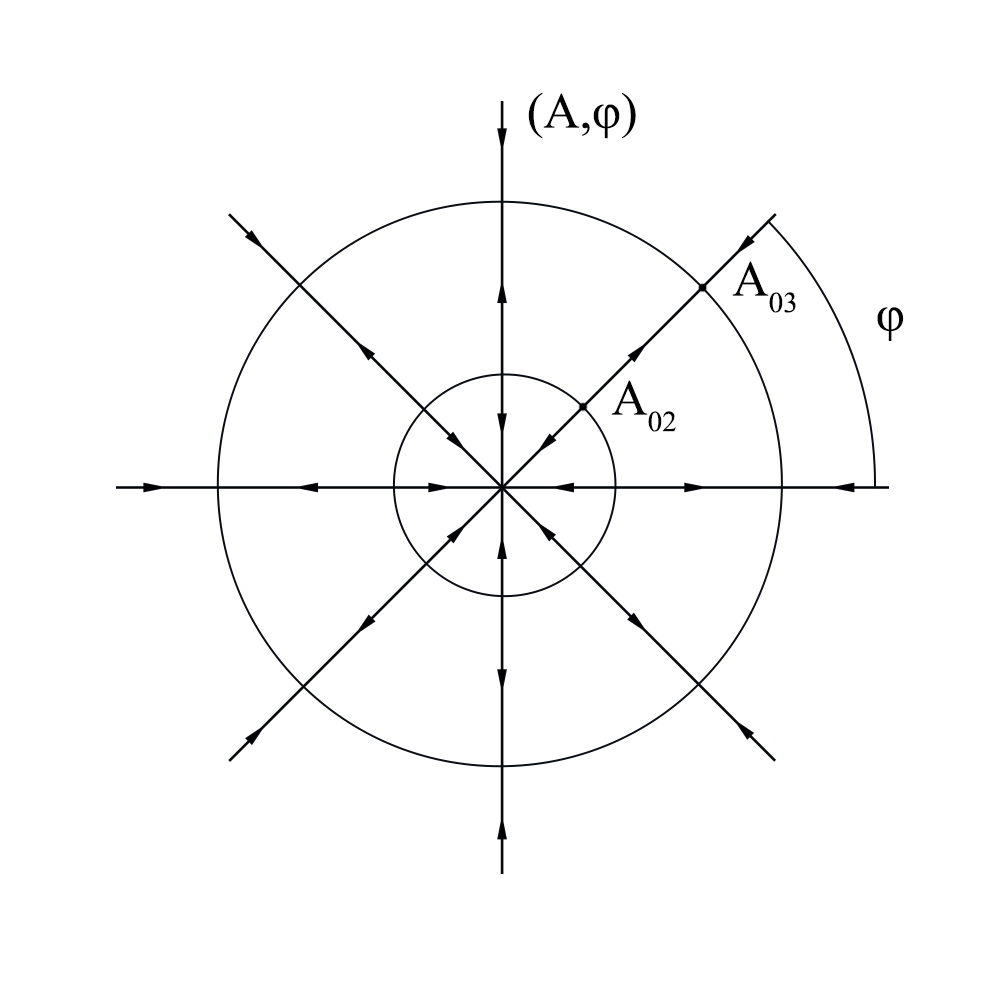
\includegraphics[width=\linewidth]{pics/Ris1.png} 
        \vspace{-50pt}
        \label{fig:1}
        \captionof{figure}{} 
    \end{minipage}
\hfill     
    \begin{minipage}{0.49\linewidth}
        \centering
        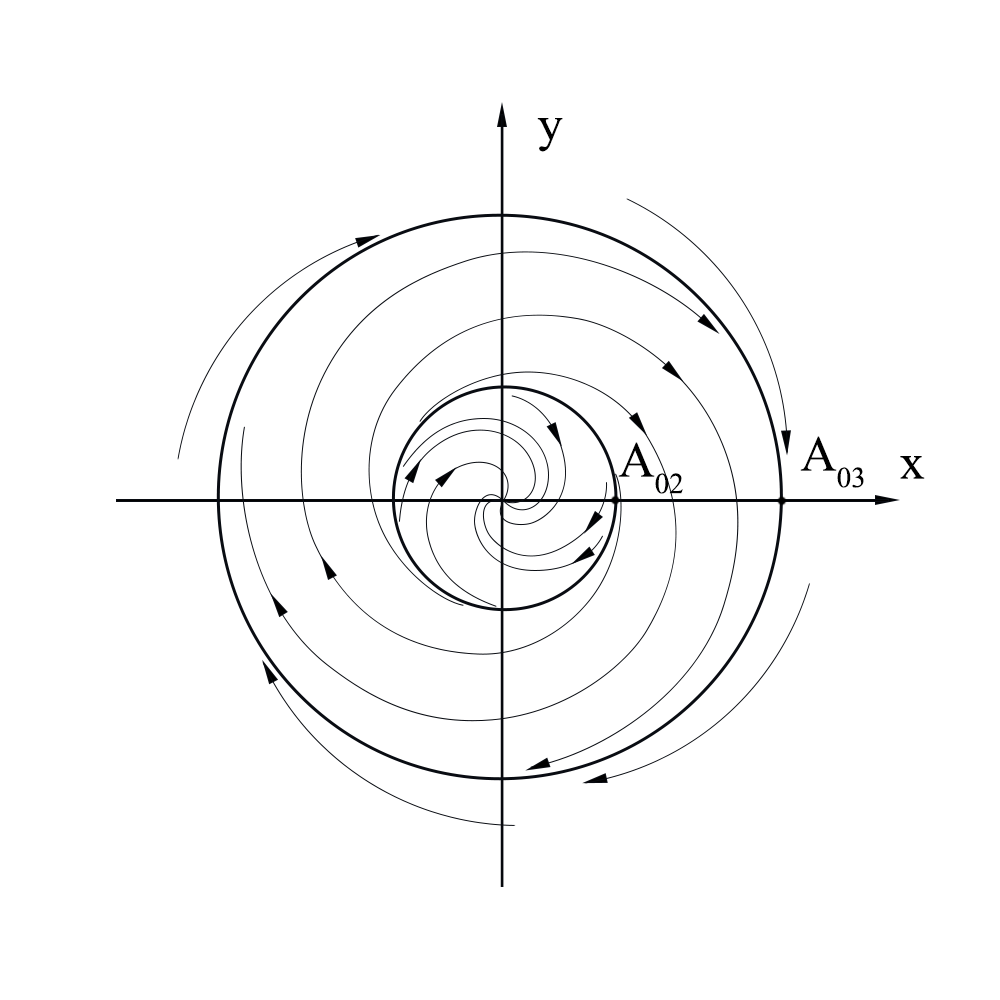
\includegraphics[width=\linewidth]{pics/Ris2.png}  
        \vspace{-50pt}
        \label{fig:2}
        \captionof{figure}{} 
    \end{minipage} 
\end{center} 

Переход к переменным xy осуществляется с помощью формул преобразования  (\ref{eq:2}). Фазовый портрет на плоскости ху может быть получен, если вращать плоскость Ван-дер-Поля по часовой стрелке с круговой частотой $\omega=1$ вокруг начала координат. Тогда окружности, состоящие из состояний равновесия, перейдут в круговой предельные циклы, имеющие те же радиусы $A_{0i}$. Предельные циклы будут устойчивы, если устойчивы состояния равновесия укороченных уравнений, и наоборот. Остальные траектории, представляющие собой отрезки прямых на плоскости переменных Ван-дер-Поля, преобразуются на плоскости ху в спирали (рис.2).

\subsection{Исходные и укороченные уравнения}

В работе исследуется LC-генератор с контуром в цепи сетки (рис.3), относящийся к разряду квазисинусоидальных автоколебательных систем.

\begin{center}
    \begin{minipage}{0.49\linewidth}
        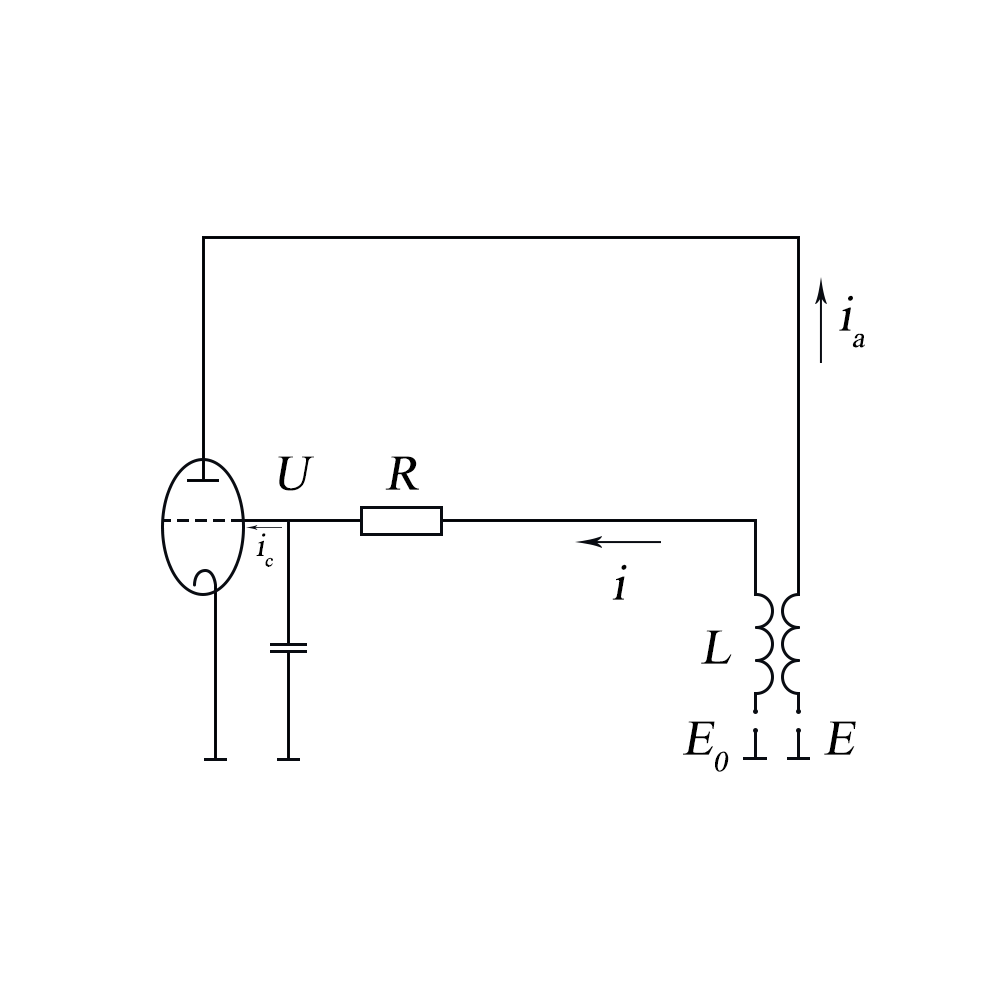
\includegraphics[width=\linewidth]{pics/Ris3.png} 
        \vspace{-60pt}
        \label{fig:3}
        \captionof{figure}{} 
    \end{minipage}
\hfill     
    \begin{minipage}{0.49\linewidth}
        \centering
        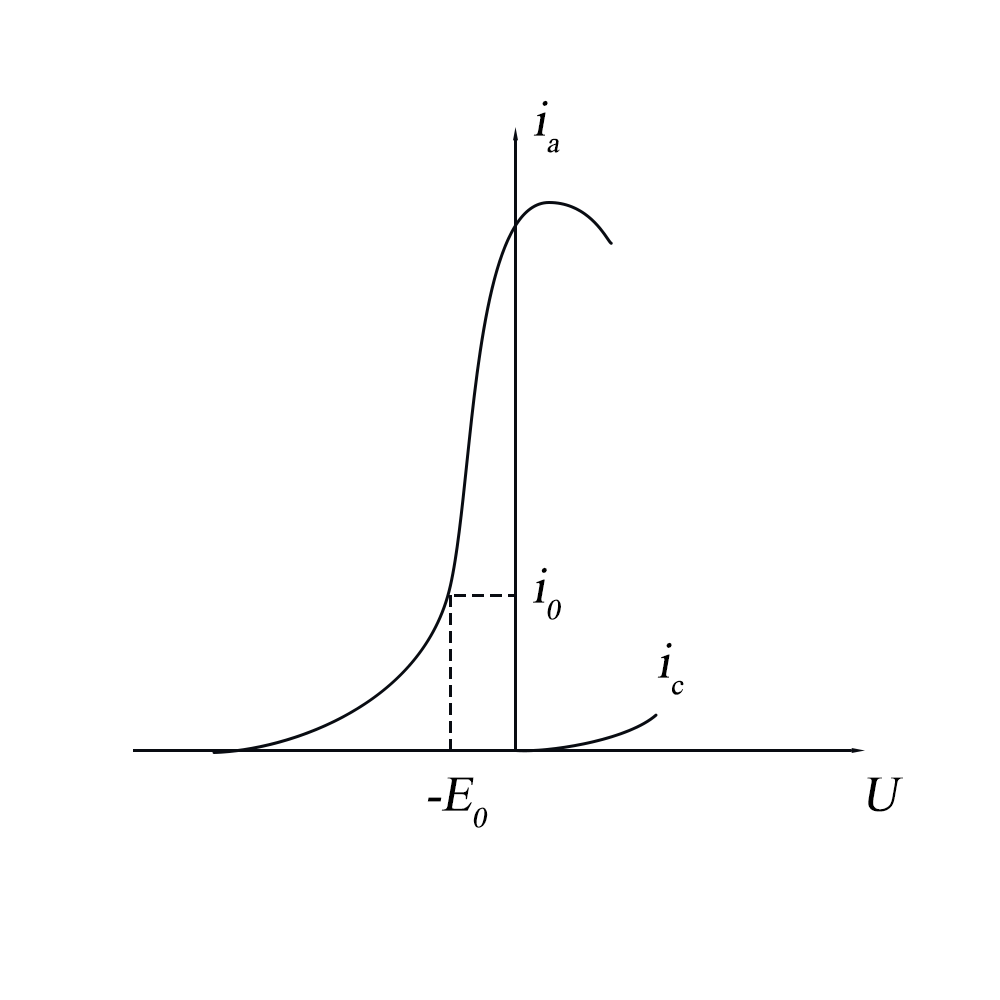
\includegraphics[width=\linewidth]{pics/Ris4.png}  
        \vspace{-60pt}
        \label{fig:4}
        \captionof{figure}{} 
    \end{minipage} 
\end{center}   

Отправной точкой теоретического исследования этой системы являются уравнения Кирхгофа, которые, с учетом обозначений, принятых на рис.3, запишутся в виде:
\begin{gather}
\label{eq:9}
L\frac{di}{dt}+Ri+U=M\frac{di_a}{dt}-E_0,\\\notag
i=C\frac{dU}{dt}+i_c,
\end{gather}
где $i_a$ и $i_c$ - анодные и сеточные токи лампы, зависящие в общем случае от анодного и сеточного напряжений. В дальнейшем будем учитывать их зависимость только от сеточных напряжений, то есть пренебрежем реакцией анода. Качественный вид анодно-сеточной и сеточной характеристик приведен на рис.4. В проводимом рассмотрении эти нелинейные функции будут аппроксимированы полиномами. 

Исключив из системы (\ref{eq:9}) ток и введя новые переменные
\begin{equation}
\label{eq:10}
x=U+E_0, ~ \tau=\frac{t}{\sqrt{LC}},
\end{equation}
запишем исходную систему  (\ref{eq:9}) в виде одного уравнения второго порядка
\begin{equation}
\label{eq:11}
\ddot{x}+x=\frac{d}{d\tau}[-\delta x+\sigma f_1(x)]-f_2(x)
\end{equation}

Здесь $\sigma=\frac{M}{\sqrt{LC}}>0$, $\alpha=\frac{L}{M}$, $\delta=R\sqrt{\frac{C}{L}}$, $f_1=(i_a-\alpha i_c)$, $f_2=Ri_c$. Заметим, что функция $f_1(x)$ включает в себя разность анодного и сеточного токов, но т.к. сеточный ток меньше анодного, то не будет большой ошибкой считать $f_1=i_a$.

Укороченные уравнения для данной системы будут иметь вид:
\begin{gather}
\label{eq:12}
\dot\rho=-\frac{1}{2} (\delta-\sigma \bar{f_1}(\rho^2))\rho,\\\notag
\dot\varphi=\frac{1}{2}\bar{f_2}(\rho^2).
\end{gather}

Здесь $\bar{f_1}(\rho^2)$  определяется анодно-сеточной характеристикой лампы и влияет на условия возбуждения генератора и амплитуду установившихся колебаний;  $\bar{f_2}(\rho^2)$ определяется сеточной характеристикой и влияет на поправку к частоте. Для отыскания установившихся (стационарных) значений амплитуды автоколебаний достаточно найти устойчивые состояния равновесия  $\bar{\rho}$  первого из уравнений системы (\ref{eq:12}). При этом из второго уравнения системы найдем поправку к частоте автоколебаний:
\begin{equation}
\label{eq:13}
\Delta \omega=\frac{\bar{f_2}(\bar{\rho}^2)}{2}
\end{equation}

задающую величину, на которую частота колебаний генератора будет отличатся от частоты колебаний контура. Тем самым, в режиме установившихся автоколебаний будем иметь:

\begin{equation}
\label{eq:14}
\varphi=\frac{\bar{f_2}(\bar{\rho}^2)}{2}\tau+\varphi_0
\end{equation}

\begin{equation}
\label{eq:15}
x=2\bar{\rho}\cos(\tau+\varphi)=2\bar{\rho}\cos[(1+\frac{\bar{f_2}(\bar{\rho})}{2})\tau+\varphi_0].
\end{equation}

\subsection{Стационарные режимы работы генератора}

Прежде чем переходить к изучению различных режимов работы лампового генератора, выясним, при каких условиях справедлива та или иная аппроксимация нелинейной характеристики лампы. На динамику генератора и стационарные режимы его работы влияют только нечетные члены степенного ряда нелинейной характеристики $f_{1}(x)$. Выделим из нелинейной функции нечетную ее часть с помощью соотношения
\begin{equation}
\vspace{0pt}
\label{eq:16}
f_H(x)=\frac{f(x)-f(-x)}{2}
\end{equation}

Вид нечетной части характеристики, а, следовательно, и возможная её аппроксимация зависят от выбора рабочей точки, положение которой определяется постоянным смещением $E_{0}$ на сетке лампы. Рассмотрим возможные аппроксимации нелинейной функции $f_{1}$ и, как следствие, различные режимы работы генератора.

{\bfseries 1.} Напряжение смещения $E_{0}$ на управляющей сетке лампы (рабочая точка) выбрано так, что нечетная часть анодно-сеточной характеристики имеет вид,  приведенный на рис.5. Это возможно в том случае, когда напряжение смещения задано в точке максимальной крутизны характеристики. При этом функцию $f_{1}$ достаточно точно можно представить в виде полинома третьей степени, причем аппроксимация будет справедлива для части кривой, обозначенной сплошной линией на рис.5:
\begin{wrapfigure}{r}{.4\textwidth}
    \begin{center}
        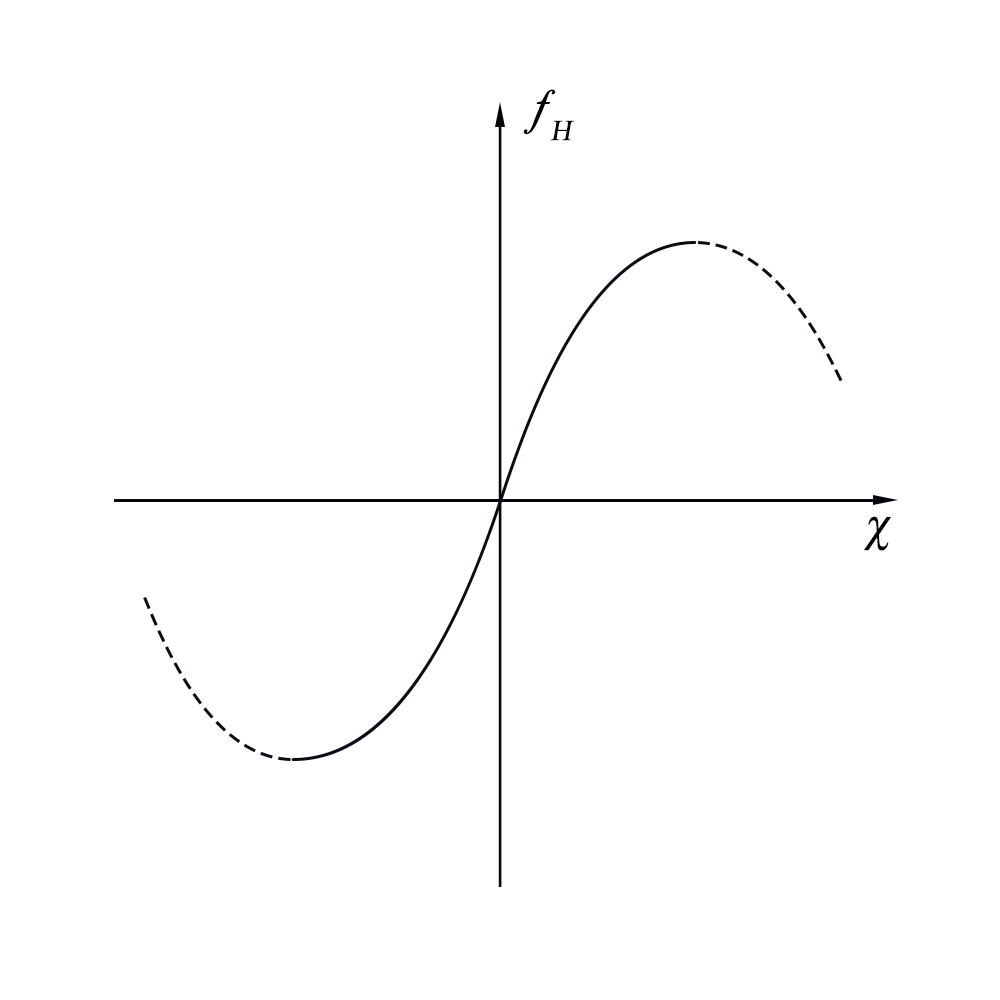
\includegraphics[width=\linewidth]{pics/Ris5.png} 
        \vspace{-40pt}
        \label{fig:5}
        \captionof{figure}{} 
    \end{center}
\end{wrapfigure}   
\begin{equation}
\label{eq:17}
f_1(x)=a_1+\frac{a_2}{2}x^2-\frac{a_3}{6}x^3
\end{equation}

Здесь и в дальнейшем все коэффициенты аппроксимирующего полинома будем считать положительным. Для аппроксимации (\ref{eq:17}) средняя крутизна анодно-сеточной характеристики, т.е. функция $\bar{f}_1$ примет вид:
\begin{equation}
\label{eq:18}
\bar{f}_1(\rho^2)=a_1-\frac{a_3}{2}\rho^2.
\end{equation}

В этом случае закон изменения амплитуды колебаний, согласно системе (\ref{eq:12})  будет определяться следующим уравнением: 

\begin{equation}
\label{eq:19}
\dot\rho=-\rho \bar{F}(\rho),
\end{equation}

где $\bar{F}(\rho)=\frac{[\delta-\sigma(a_1-\frac{a_3}{2}\rho^2)]}{2}$. Приравнивая правую часть этого уравнения нулю, получим стационарные значения амплитуд колебаний:
\begin{equation}
\label{eq:20}
\bar{\rho}_1=0,~ \bar{\rho}_2=\sqrt\frac{2(-\delta+\sigma a_1)}{\sigma a_3}.
\end{equation}

Их устойчивость определяется корнями следующего характеристического уравнения:

\begin{equation}
\label{eq:21}
\rho=\frac{d}{d\rho}[-\rho\bar{F}(\rho)]\bigg|_{\rho=\bar{\rho}}=-\bar{F}(\bar{\rho})-\bar{\rho}\bar{F}^{'}(\bar{\rho})
\end{equation}

Состояние системы с нулевым значением $\bar{\rho}$ (невозбужденный генератор) будет устойчивым при $\bar{F}(0)>0$, т.е. при $\sigma=\frac{\delta}{a_1}$ и неустойчивым в противном случае. Второе стационарное состояние устойчиво, если $\bar{F}^{'}(\bar{\rho})=\sigma a_3 \bar{\rho_2}>0$, что выполняется при выбранных знаках коэффициентов. Выражение (\ref{eq:21}) определяет зависимость амплитуды колебаний от линейного декремента $\delta=\frac{R\sqrt{C}}{\sqrt{L}}$, коэффициента связи $\sigma=\frac{M}{\sqrt{LC}}>0$, и коэффициентов аппроксимации анодно-сеточной характеристики $a_1$ и $a_3$. Можно построить бифуркационные диаграммы, выражающие зависимость $\bar{\rho}_2$ от любого из перечисленных параметров. Зависимость $\bar{\rho}_2$ от параметра $\sigma$ (величина обратной связи) приведена на рис.6, где точками обозначены устойчивые состояния, а крестиками - неустойчивые. из приведенной диаграммы видно, что схема возбуждается при условии $\sigma>\frac{\delta}{a_1}$, или, если перейти к параметрам схемы, при $M>\frac{RC}{a_1}$. В этом неравенстве величина $a_1$ - крутизна анодно-сеточной характеристики в рабочей точке. Точка $\sigma=\frac{\delta}{a_1}$ на бифуркационной диаграмме называется {\itshapeточкой бифуркации} - здесь качественно меняется поведение системы.
\begin{center}
    \begin{minipage}{0.3\linewidth}
        \begin{minipage}[t]{\linewidth}
                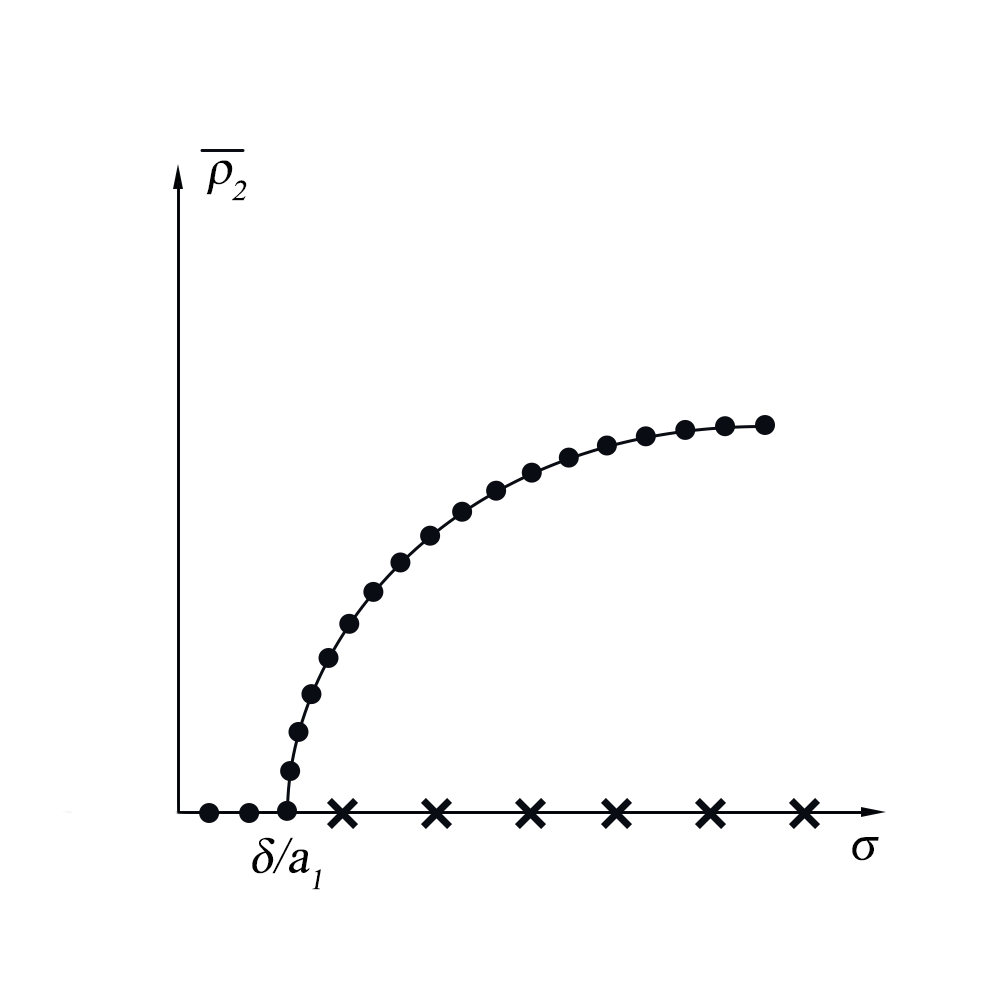
\includegraphics[width=\linewidth]{pics/Ris6.png} 
                \vspace{0pt}
                \label{fig:6}
                \captionof{figure}{} 
        \end{minipage}
    \end{minipage}
    \begin{minipage}[t]{0.6\linewidth}
            \begin{minipage}{0.45\linewidth}
                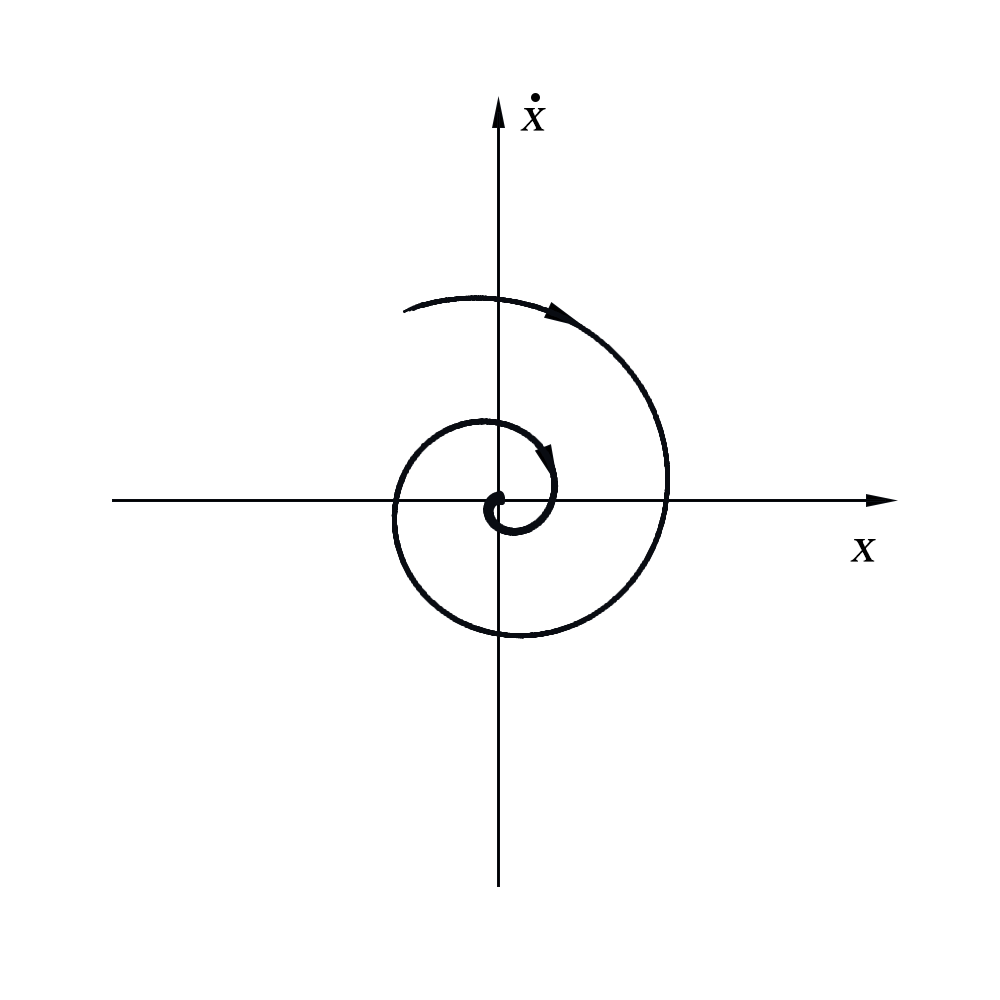
\includegraphics[width=\linewidth]{pics/Ris7a.png} 
                \vspace{-30pt}
                \label{fig:7}
                \captionof{subfigure}{} 
            \end{minipage}
            \begin{minipage}{0.45\linewidth}
                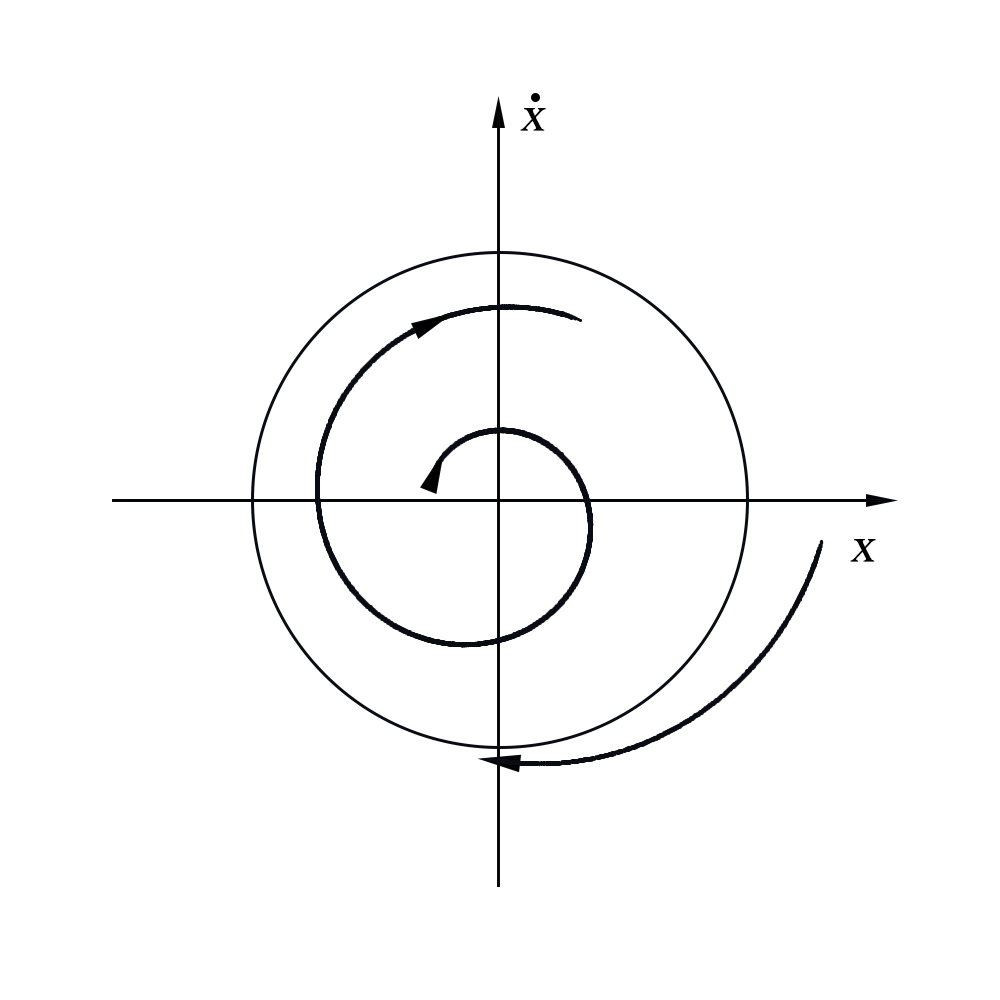
\includegraphics[width=\linewidth]{pics/Ris7b.png} 
                \vspace{-30pt}
                \label{fig:8}
                \captionof{subfigure}{} 
            \end{minipage}
            \captionof{figure}{}
    \end{minipage}
\end{center}
  
Фазовые портреты системы при $\sigma<\frac{\delta}{a_1}$ и $\sigma>\frac{\delta}{a_1}$ приведены на рис.7 a и b. Как видно из рис.6 и рис.7 b, 
предельный цикл устанавливается при сколь угодно малых начальных условиях, то есть генератор обладает {\itshapeмягким режимом} возбуждения по 
отношению к начальным условиям. Термин "мягкий" может употребляться в другом смысле - в качестве характеристики типа генератора, отличающегося 
плавным нарастанием установившегося значения амплитуды колебаний при медленном и непрерывном изменении параметра обратной связи. Приведенная на рис.6 
бифуркационная диаграмма соответствует именно такому типу генератора.  

{\bfseries 2.} Рабочая точка выбрана так, что нечетная часть характеристики имеет вид,
\begin{wrapfigure}{r}{.4\textwidth}
    \begin{center}
        \vspace{-10pt}
        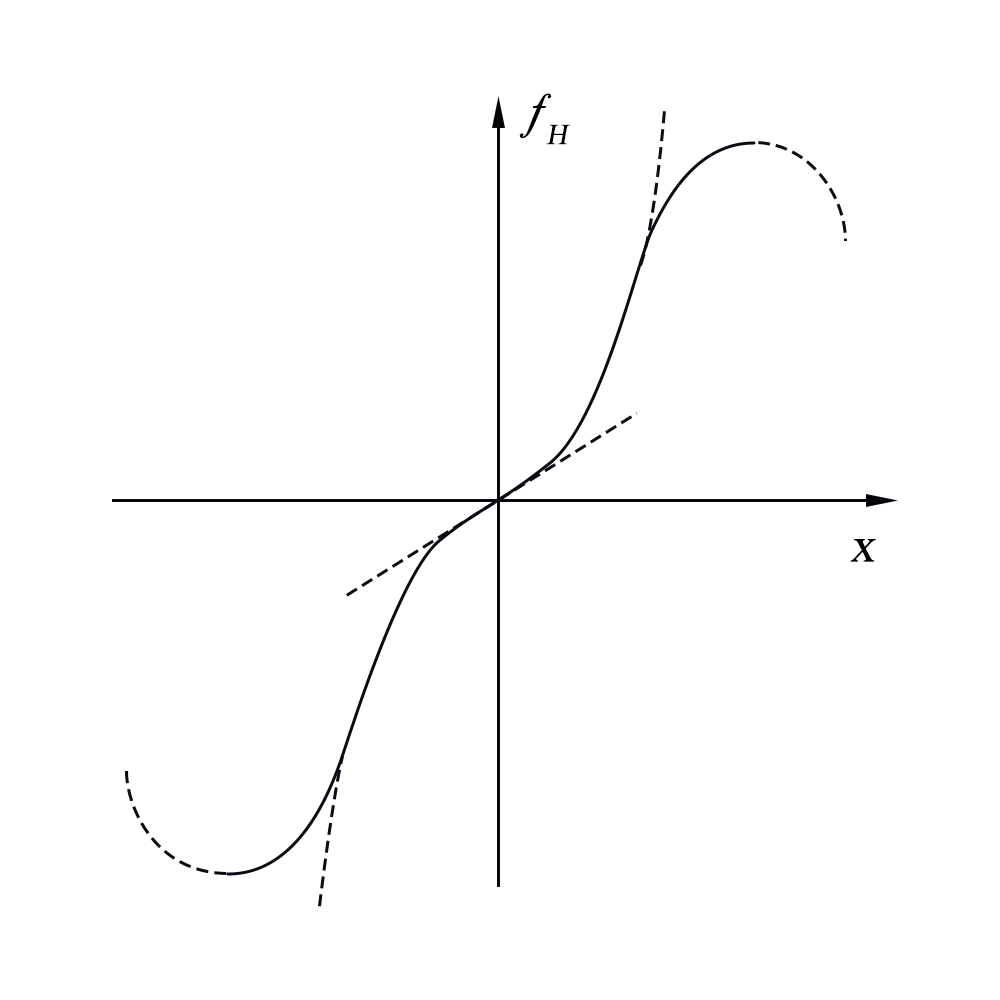
\includegraphics[width=\linewidth]{pics/Ris8.png} 
        \vspace{-40pt}
        \label{fig:8}
        \captionof{figure}{}
        \vspace{20pt} 
    \end{center}
\end{wrapfigure}
приведенный на рис.8.
 Этому случаю чаще всего отвечают напряжения смещения, близкие к напряжению осечки лампы. При этом характеристику
  лампы необходимо аппроксимировать полиномом не ниже пятой степени. Такой аппроксимации соответствует средняя крутизна 
\begin{equation}
\label{eq:22}
\bar{f}_1(\rho^2)=a_1+\frac{a_3}{2}\rho^2-\frac{a_5}{12}\rho^4.
\end{equation}
и, следовательно, уравнение, определяющее стационарные значения амплитуды автоколебаний принимает вид
\begin{equation}
\label{eq:23}
\rho[\delta-\sigma(a_1+\frac{a_3}{2}\rho^2-\frac{a_5}{12}\rho^4)]=0.
\end{equation}

\begin{wrapfigure}{l}{.4\textwidth}
    \begin{center}
        \vspace{-30pt}
        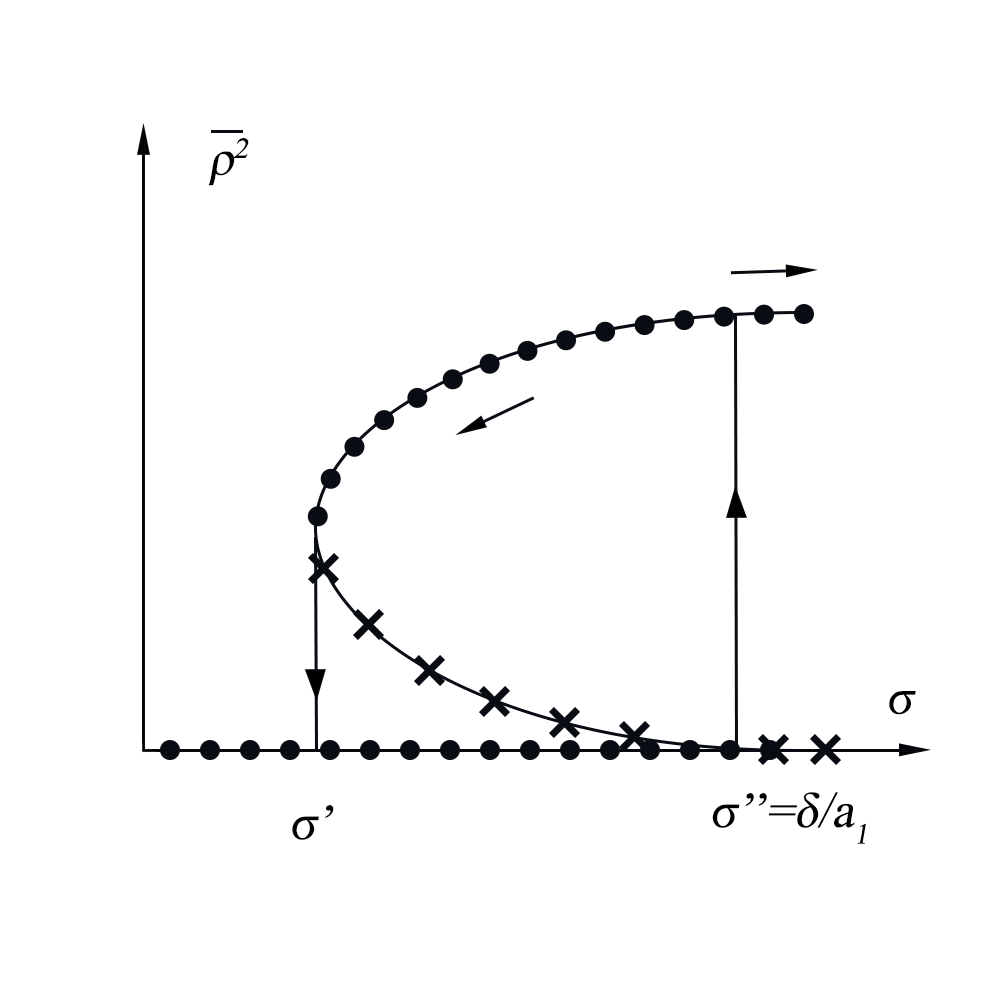
\includegraphics[width=\linewidth]{pics/Ris9.png} 
        \vspace{-50pt}
        \label{fig:9}
        \captionof{figure}{} 
        \vspace{0pt}
    \end{center}
\end{wrapfigure} 
Бифуркационная диаграмма для этого случая приведена на рис.9. Из него следует, что при значениях параметра $\sigma$, лежащих в 
интервале ${\sigma}'\textless \sigma \textless {\sigma}"$, возникновение автоколебаний возможно лишь, если начальное значение 
$\rho$ превышает соответствующее пороговое значение. В этом случае говорят о {\itshapeжестком режиме} возбуждения генератора. 
Бифуркационная диаграмма, изображенная на рис.9 характеризуется гистерезисным эффектом установления срыва автоколебаний при 
непрерывном изменении параметра $\sigma$. Системы с таким видом бифуркационной диаграммы относят к жёсткому типу генераторов. 
Для них, согласно рис.9, мягкое возбуждение возможно лишь при $\sigma>\sigma^"$, т.е. за пределами области гистерезиса. 
На рис.10 a,b и c приведены фазовые портреты такого генератора для различных значений параметра $\sigma$.
\begin{center}
    \begin{figure}[H]
        \begin{minipage}{0.32\linewidth}
            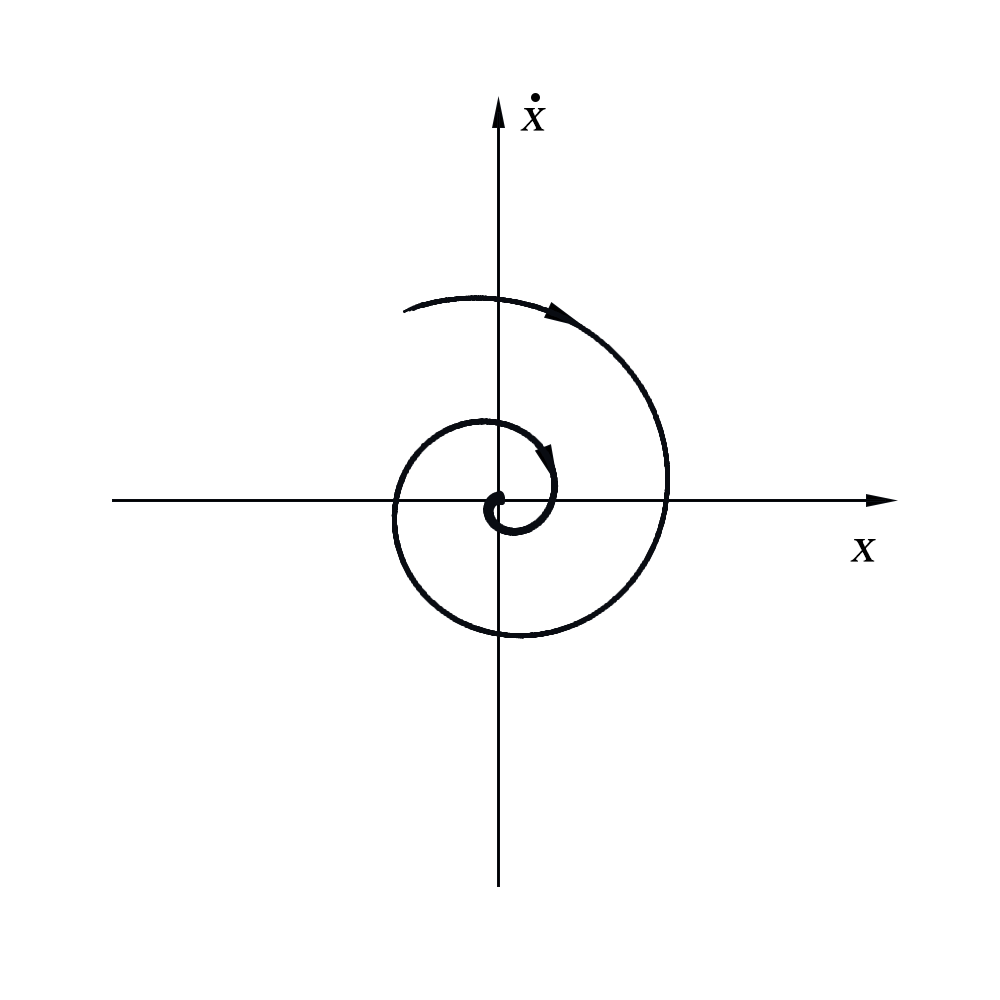
\includegraphics[width=\linewidth]{pics/Ris10a.png} 
            \vspace{-30pt}
            \label{fig:10}
            \captionof{subfigure}{} 
        \end{minipage}
    \begin{minipage}{0.32\linewidth}
        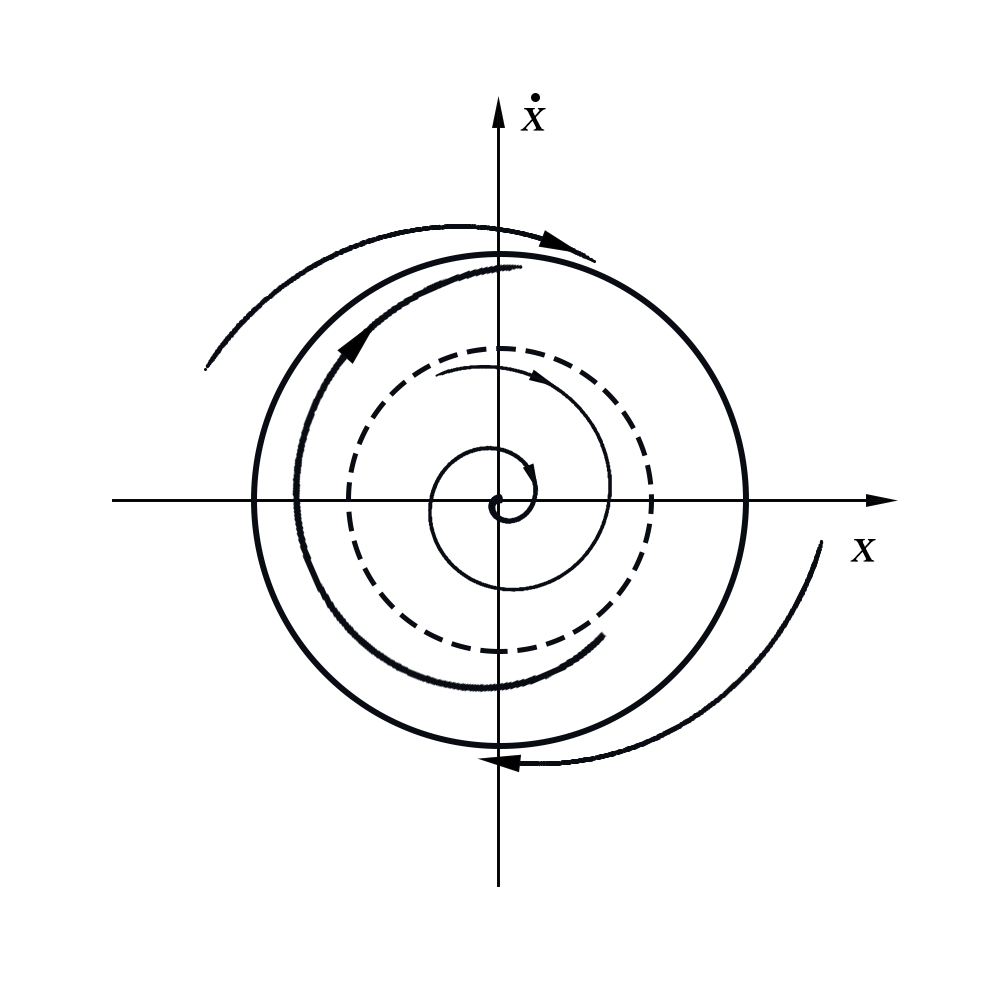
\includegraphics[width=\linewidth]{pics/Ris10b.png} 
        \vspace{-30pt}
        \label{fig:11}
        \captionof{subfigure}{} 
    \end{minipage}
    \begin{minipage}{0.32\linewidth}
        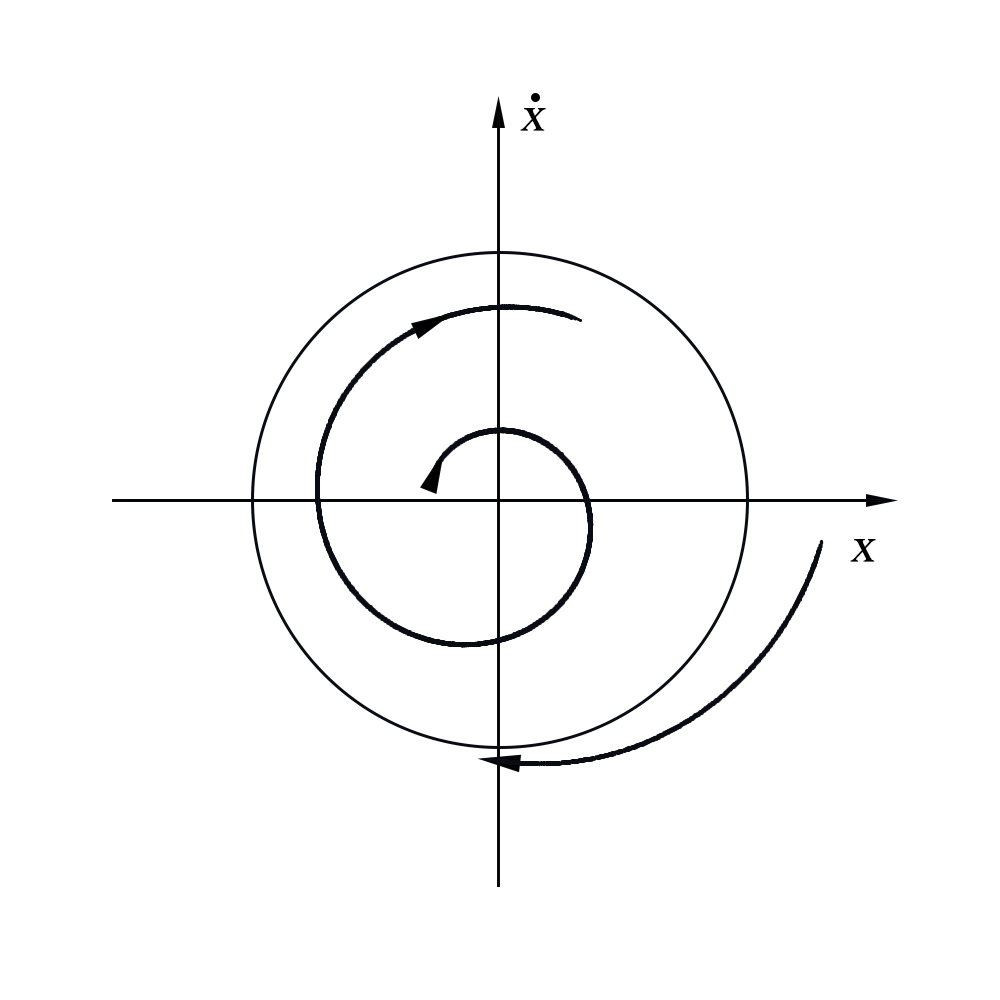
\includegraphics[width=\linewidth]{pics/Ris10c.png} 
        \vspace{-30pt}
        \label{fig:12}
        \captionof{subfigure}{} 
    \end{minipage}
    \caption{}
    \vspace{-40pt}
    \end{figure}
\end{center} 

{\bfseries 3.} Если рабочая точка выбрана при положительных напряжениях на сетке лампы, то график нечетной части нелинейной характеристики имеет вид, приведенный на рис.11.

Здесь для аппроксимации анодно-сеточной характеристики лампы необходимо использовать полином седьмой степени. 
В этом случае функция $\bar{f}_1(\rho^2)$ и уравнение для определения ненулевых состояний равновесия запишутся 
в виде $$\bar{f}_1(\rho^2)=a_1+\frac{a_3}{2}\rho^2-\frac{a_5}{12}\rho^4-\frac{a_7}{144}\rho^6,$$ $$\delta-\sigma(a_1+\frac{a_3}{2}\rho^2-\frac{a_5}{12}\rho^4-\frac{a_7}{144}\rho^6)=0.$$
При этом возможны два варианта бифуркационной диаграммы $\bar \rho^2(\sigma)$, изображенные на рис.12. 
\begin{wrapfigure}{r}{.4\textwidth}
    \begin{center}
        \vspace{-30pt}
        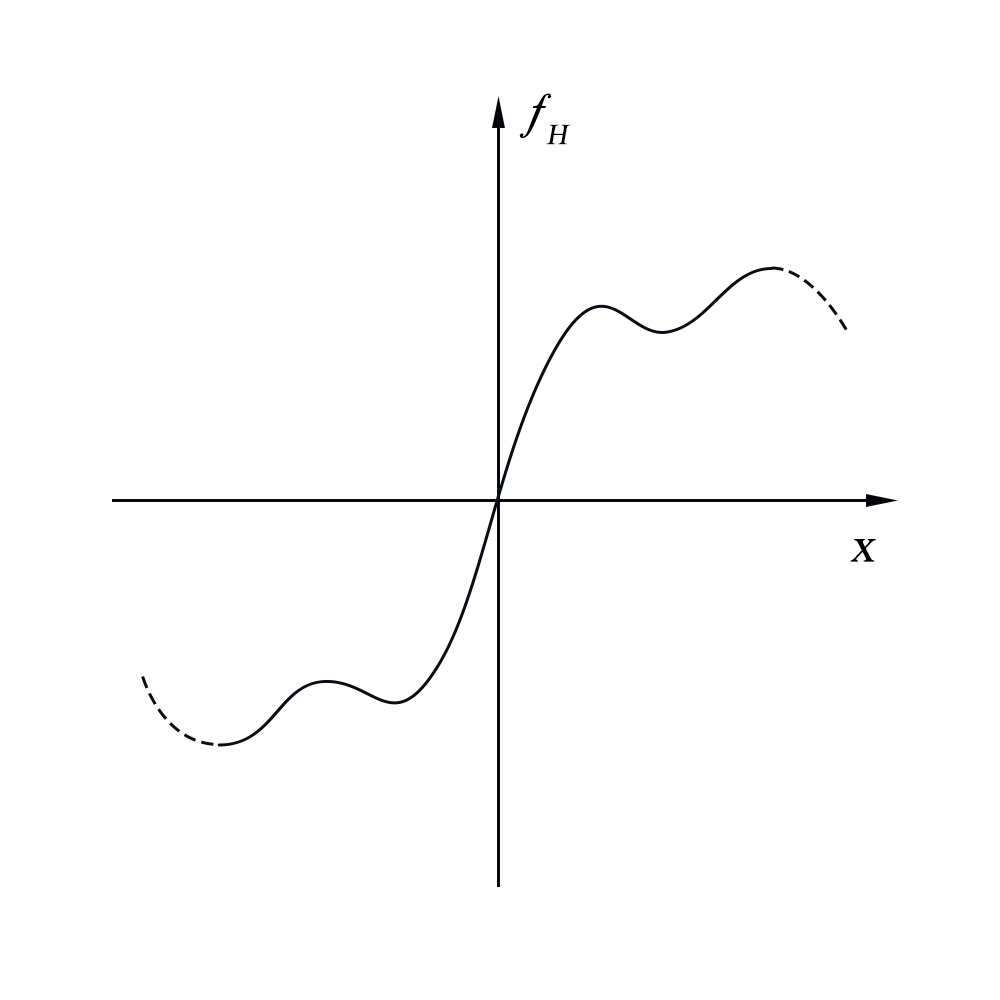
\includegraphics[width=\linewidth]{pics/Ris11.png} 
        \vspace{-50pt}
        \label{fig:9}
        \captionof{figure}{} 
        \vspace{0pt}
    \end{center}
\end{wrapfigure} 

В варианте a при уменьшении параметра $\sigma$ происходит скачкообразный переход с большего предельного цикла на меньший
 и при дальнейшем уменьшении $\sigma$ предельный цикл плавно исчезает. В варианте b при уменьшении параметра $\sigma$ до $\sigma_0$ колебания срываются до нуля. 

Описанная разновидность автоколебательных систем относится к генераторам {\itshapeсложно-жесткого типа}.
\begin{center}
    \begin{figure}[H]
        \vspace{-10pt}
        \begin{minipage}{0.49\linewidth}
            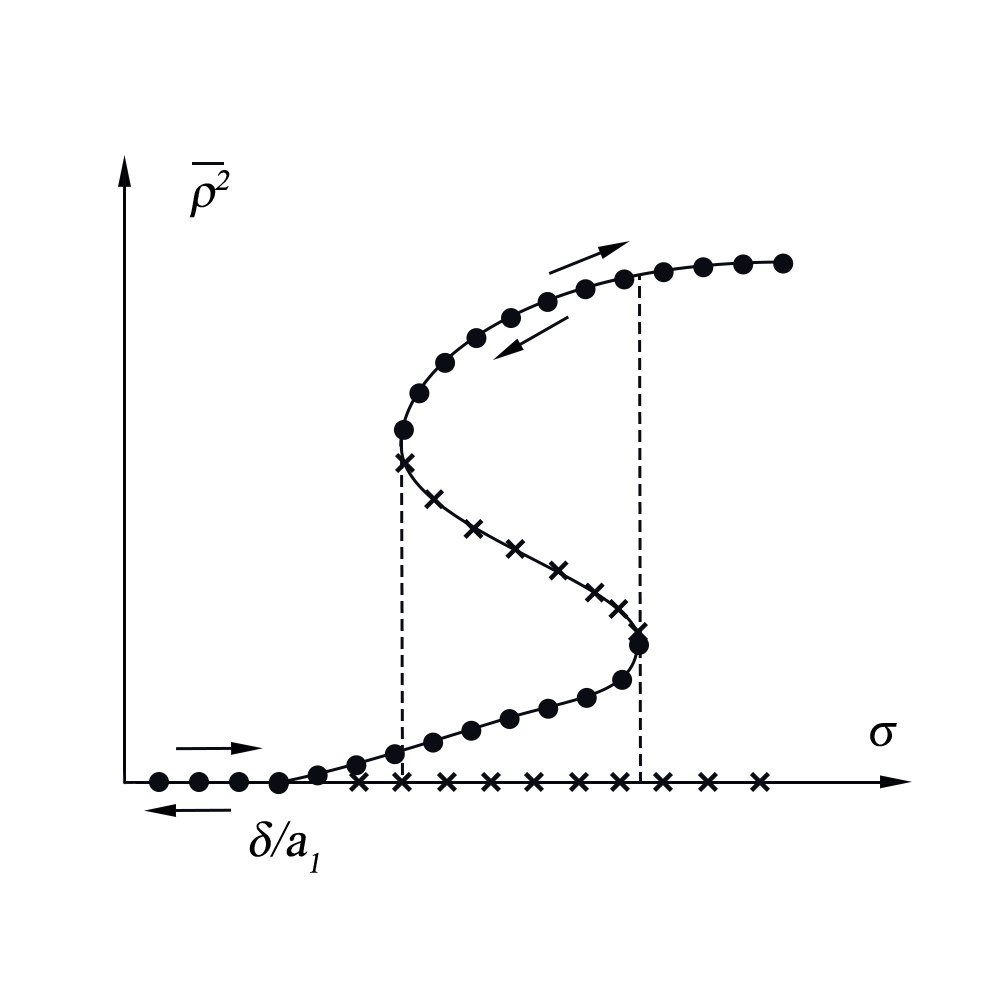
\includegraphics[width=\linewidth]{pics/Ris12a.png} 
            \vspace{-50pt}
            \label{fig:10}
            \captionof{subfigure}{} 
        \end{minipage}
    \begin{minipage}{0.49\linewidth}
        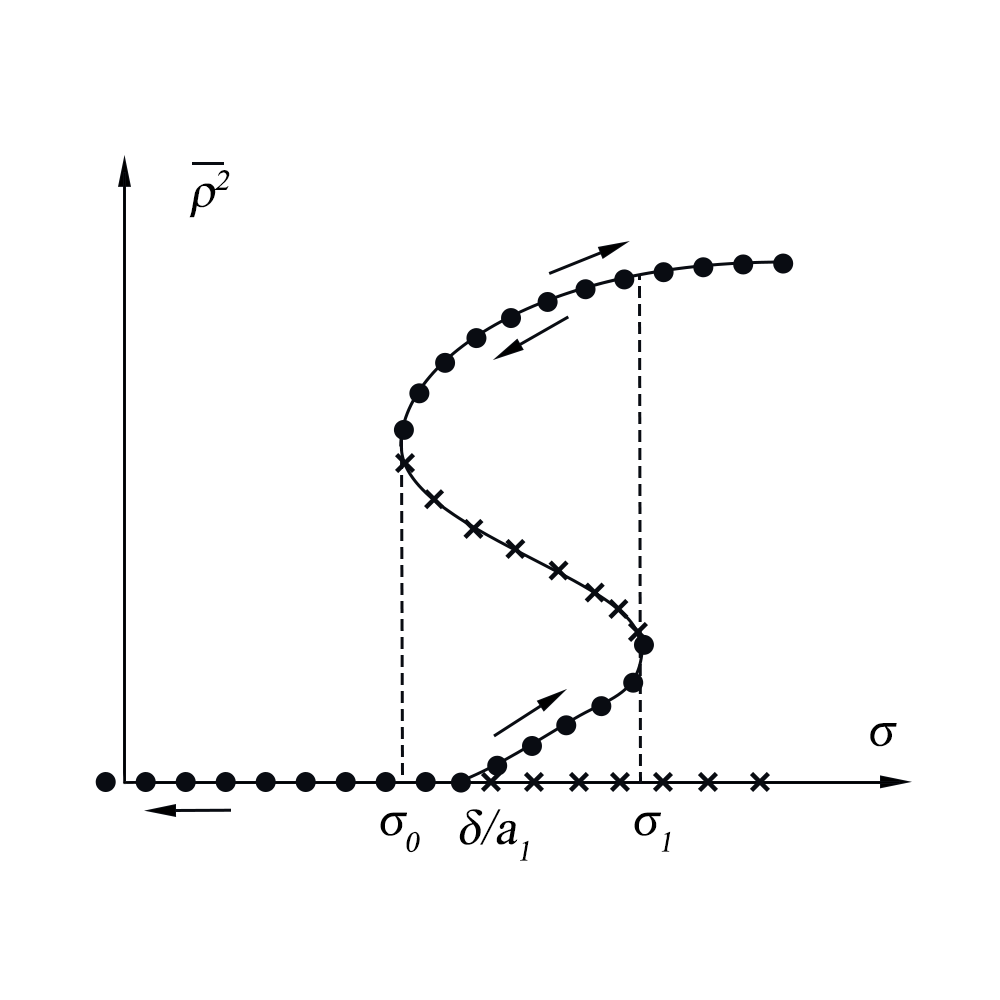
\includegraphics[width=\linewidth]{pics/Ris12b.png} 
        \vspace{-50pt}
        \label{fig:11}
        \captionof{subfigure}{} 
    \end{minipage}
    \caption{}
    \vspace{-40pt}
    \end{figure}
\end{center} 

\newpage
\section{Практическая часть}
На рис.13 приведена схема лабораторной установки.

\begin{center}
    \begin{figure}[H]
        \vspace{-10pt}
            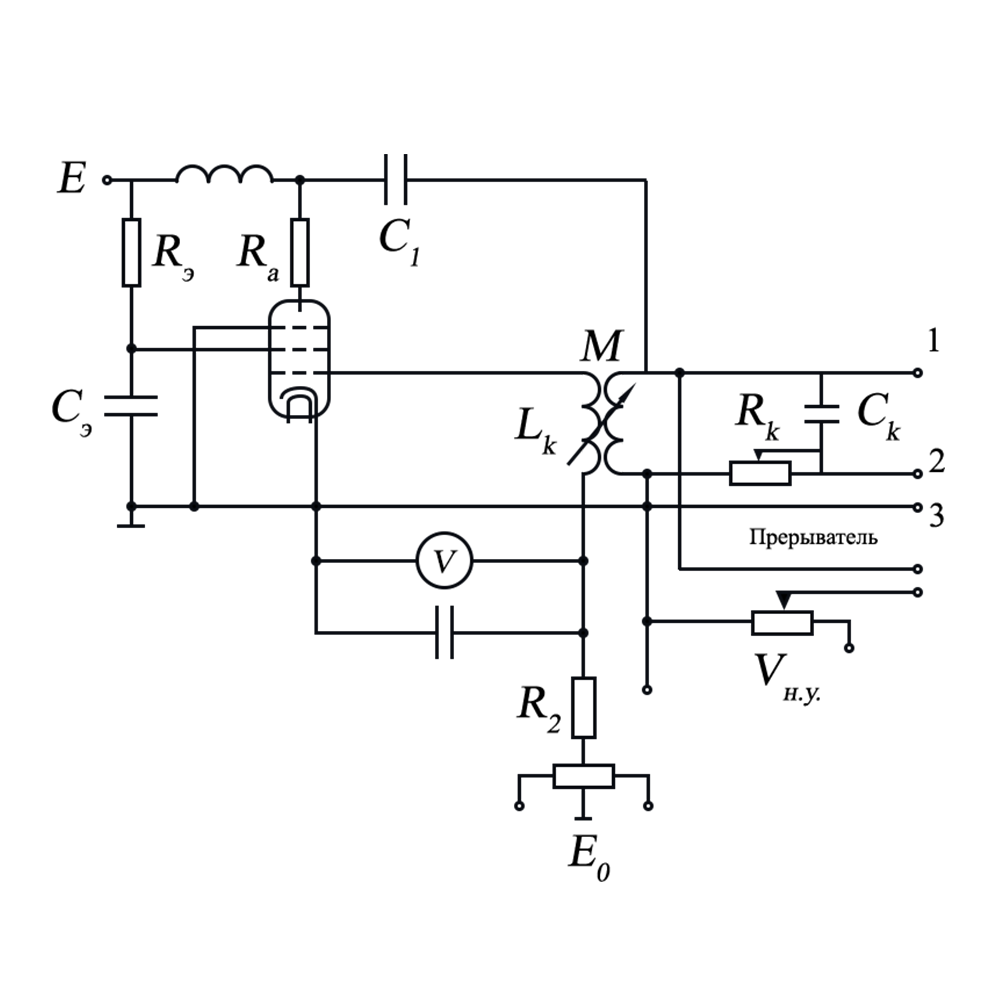
\includegraphics[width=\linewidth]{pics/scheme.png} 
            \vspace{-50pt}
            \label{fig:10}
            \captionof{figure}{} 
    \end{figure}
\end{center} 
\subsection{Мягкий режим генератора}
В данной части работы будет сниматься бифуркационная диаграмма - зависимость амплитуды от параметров системы. 
В этой работе будет изменяться коэффициент взаимной индукции $M$.

Для достижения мягкого режима работы генератора, менялось напряжение смещения $E_0$ до тех пор, пока при плавном изменении параметра $M$,
 не наблюдалось плавное изменение амплитуды. 

Снятая бифуркационная диаграмма приведена на рис. 14:
 %рис 14
 \begin{center}
    \begin{figure}[H]
        \vspace{-10pt}
            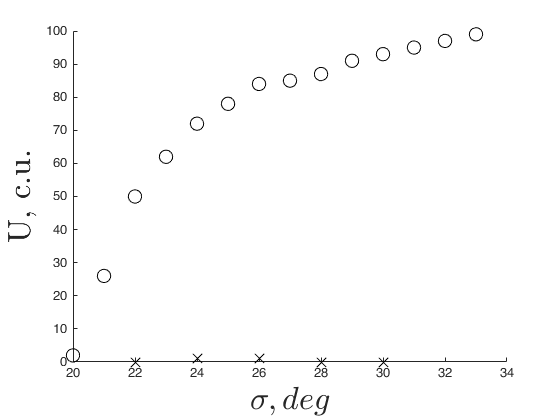
\includegraphics[]{graph/g1.png} 
            \vspace{-10pt}
            \label{fig:10}
            \captionof{figure}{Бифуркационная диаграмма для мягкого режима генератора} 
            \vspace{-20pt}
    \end{figure}
\end{center} 
По бифуркационной диаграмме было определено значение $M^{'}$ в у.е. для точки бифуркации:
$$M' = 20 \pm 1 y.e $$

Также были сняты фазовые траектории для разных начальных условий левее и правее точки бифуркации (рис.15 и рис.16).
Для наблюдения фазовых траекторий в системе включался прерыватель, позволяющий наблюдать процесс раскачки заново.

\begin{center}
    \begin{figure}[H]
        \begin{minipage}{0.49\linewidth}
            \centering
            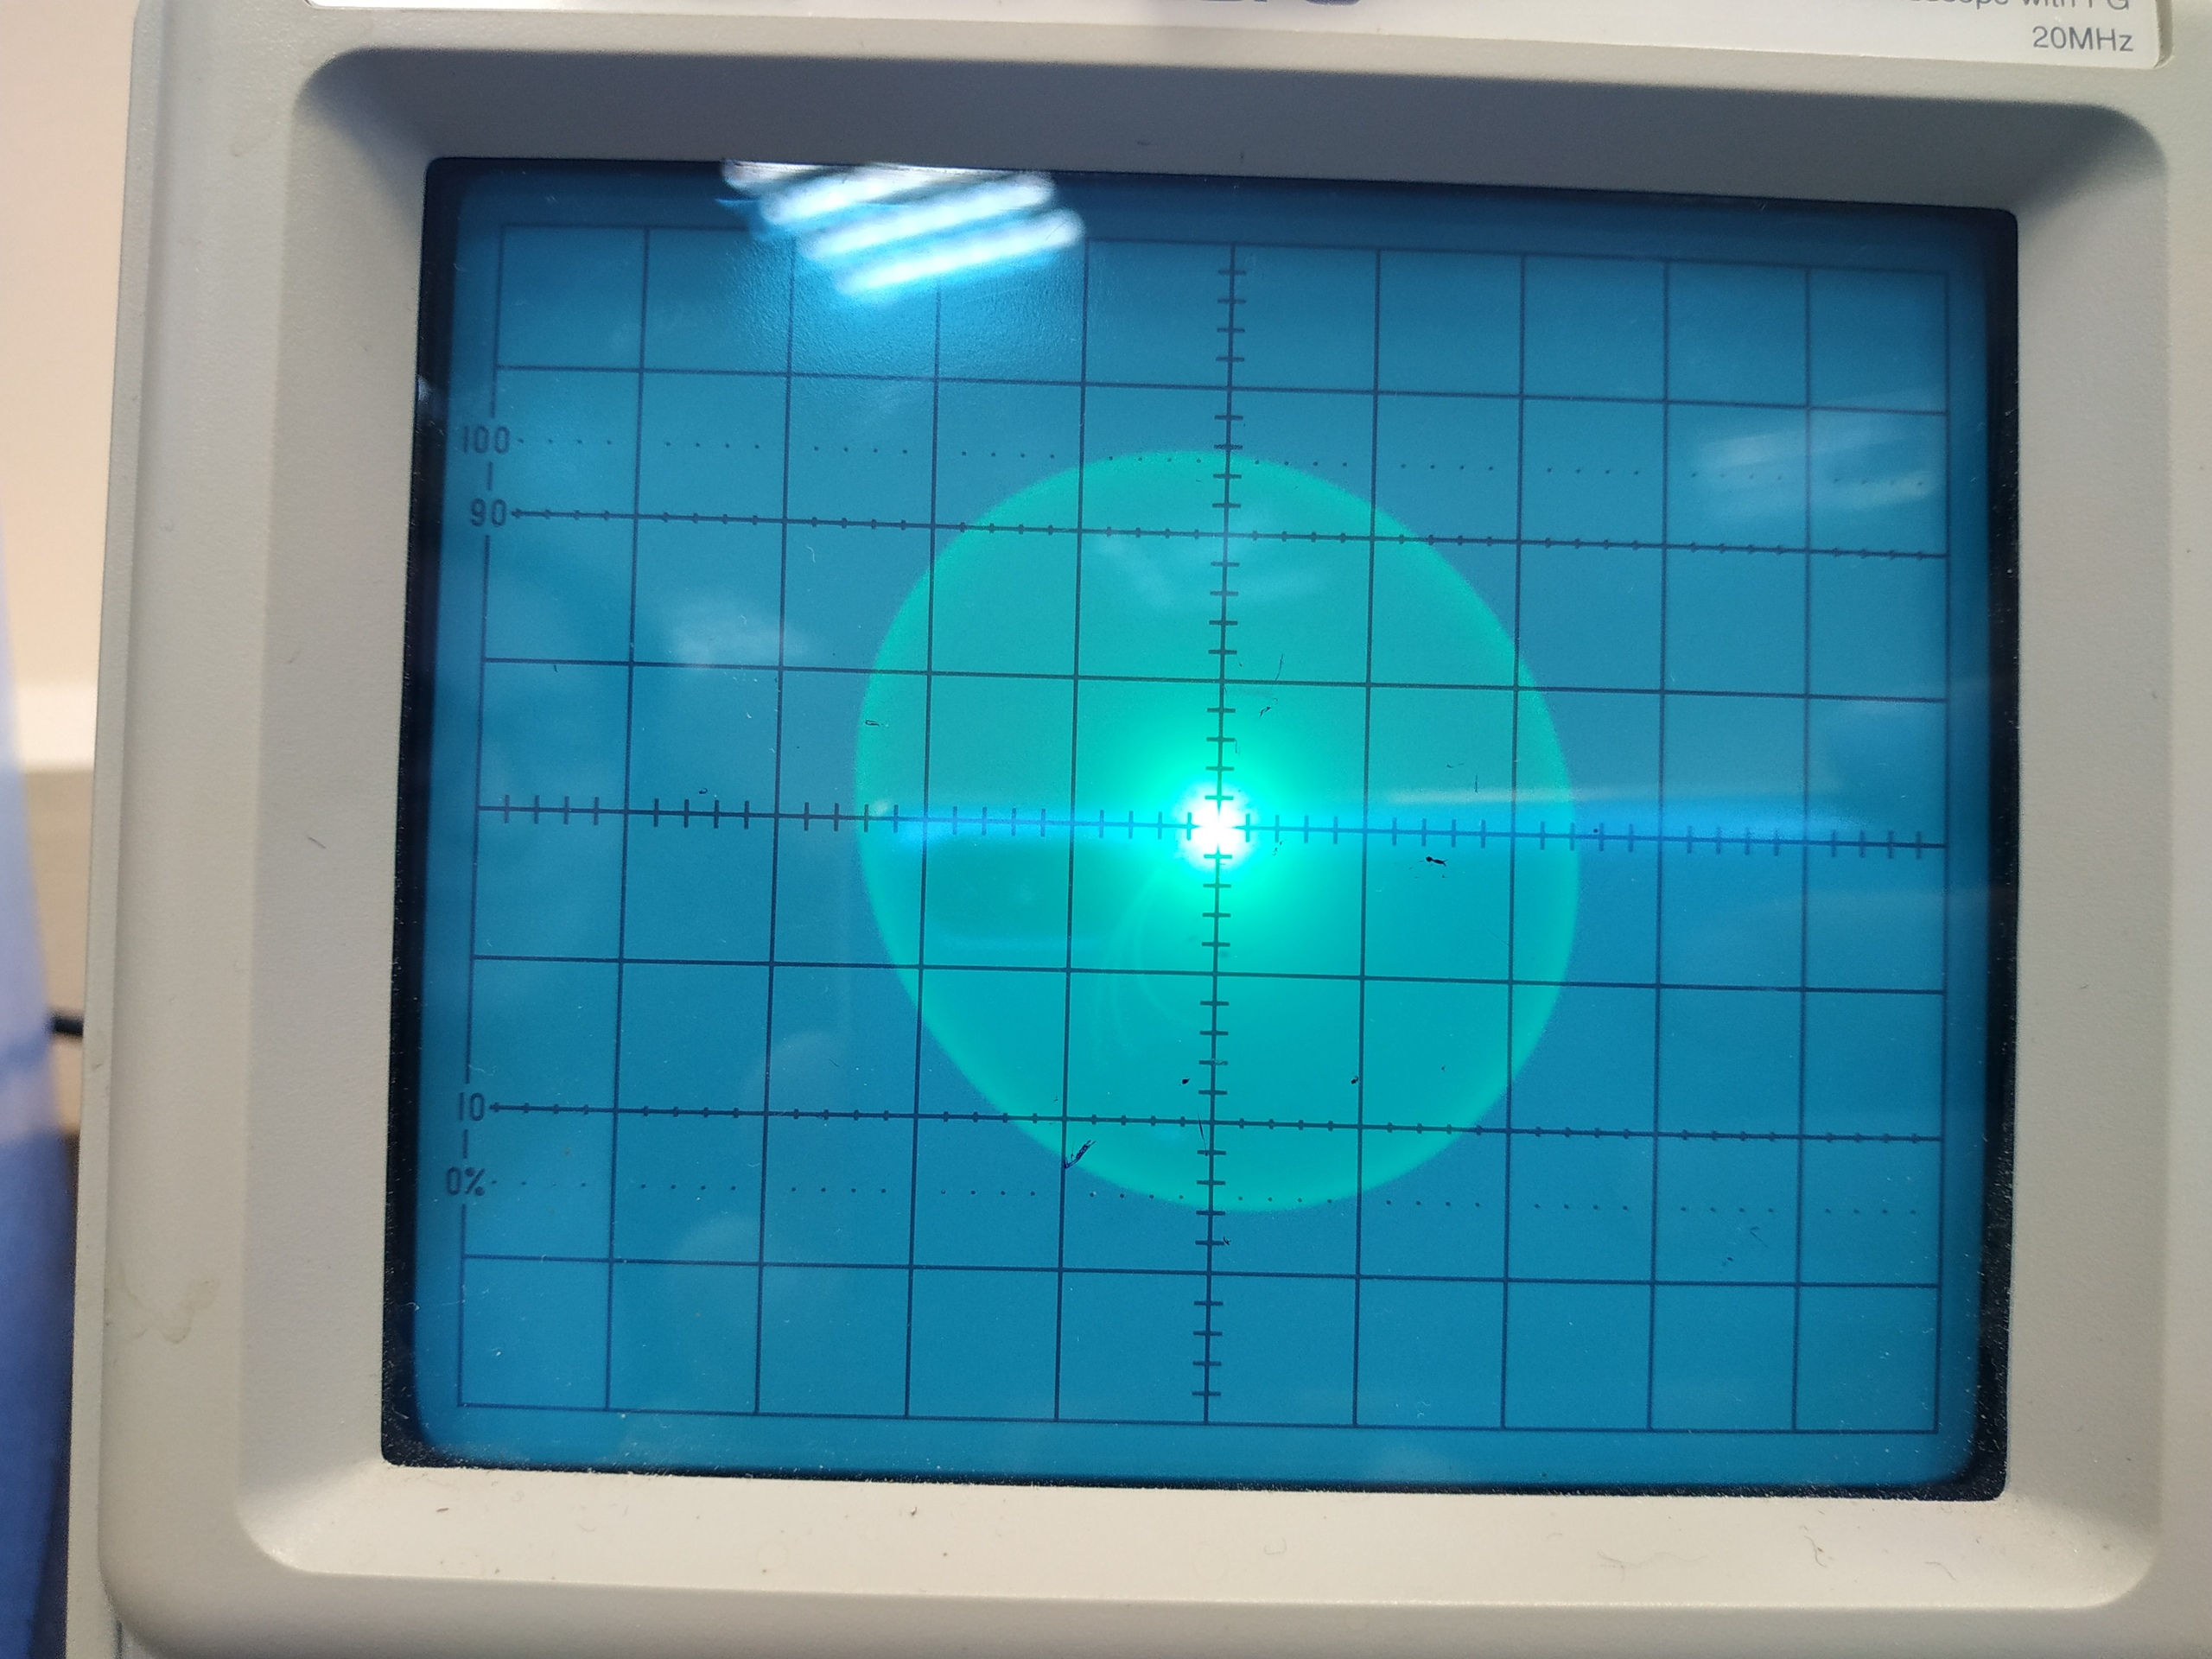
\includegraphics[height=100pt]{img/2.jpg} 
            \vspace{0pt}
            \label{fig:10}
            \captionof{subfigure}{} 
        \end{minipage}
        \begin{minipage}{0.49\linewidth}
            \centering
            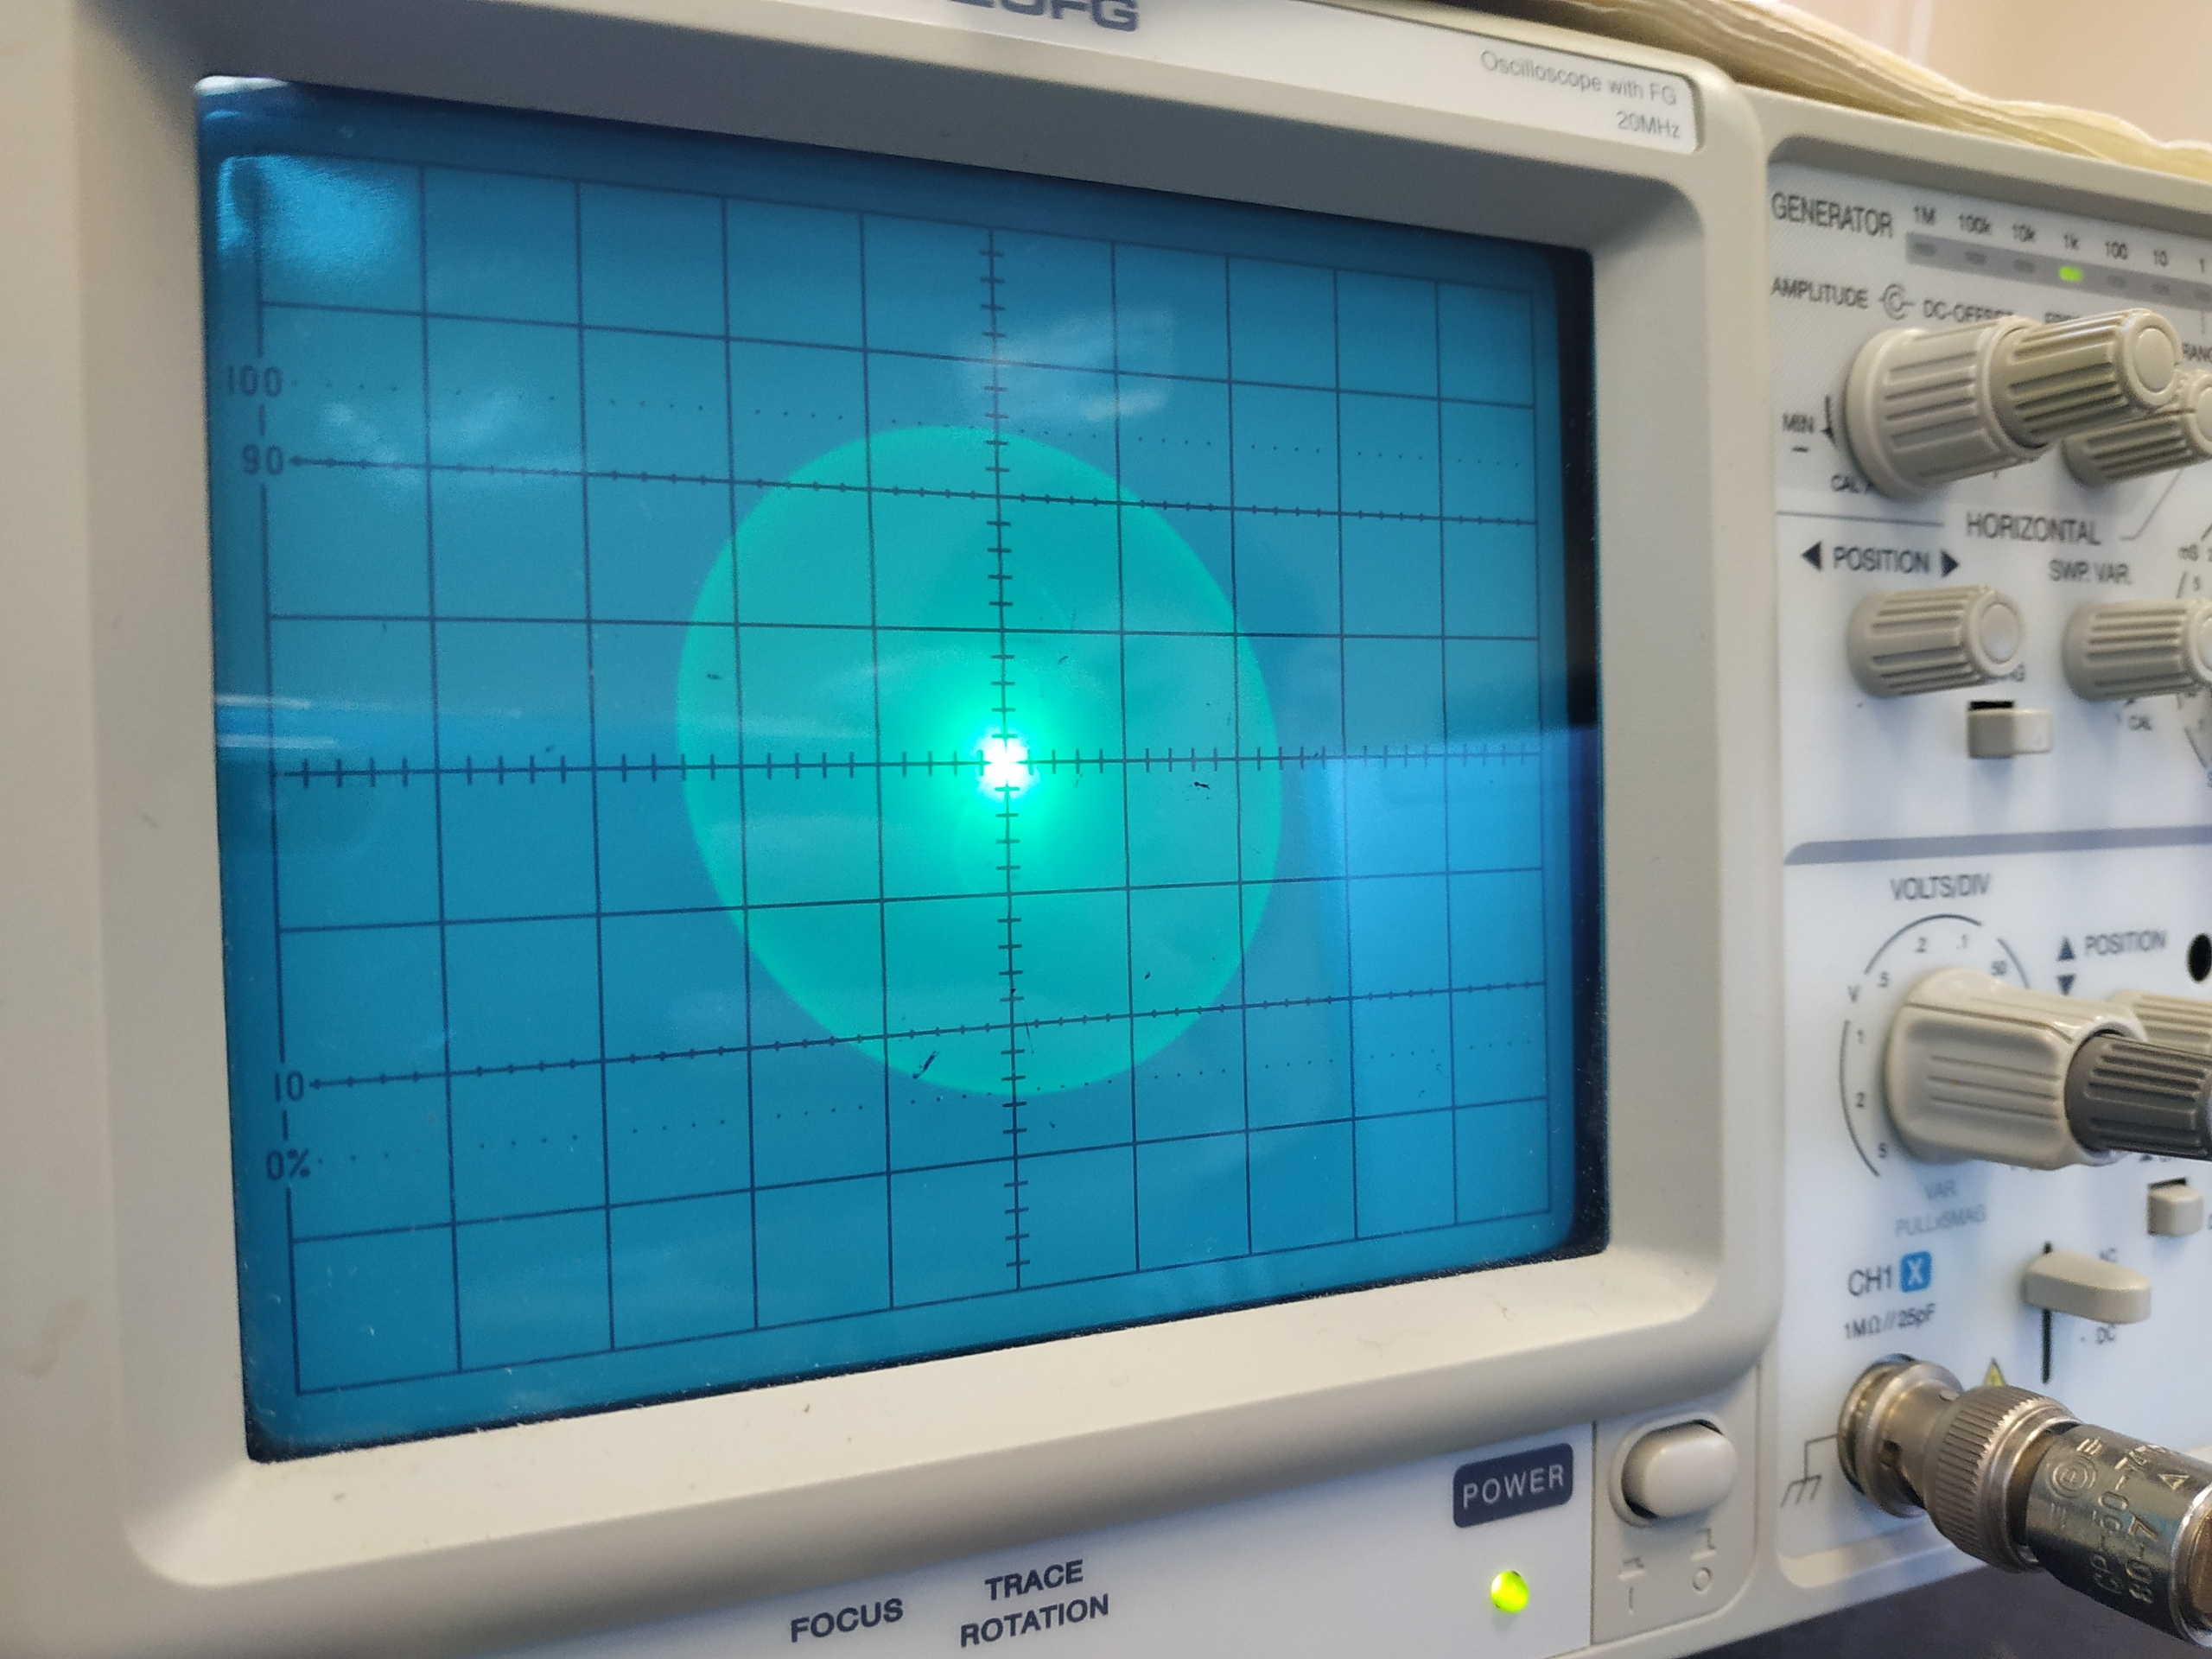
\includegraphics[height=100pt]{img/1.jpg} 
            \vspace{0pt}
            \label{fig:11}
            \captionof{subfigure}{} 
        \end{minipage}

    \caption{Фазовая траектория левее точки бифуркации}
    \vspace{-40pt}
    \end{figure}
\end{center} 

\begin{center}
    \begin{figure}[H]
        \begin{minipage}{0.32\linewidth}
            \centering
            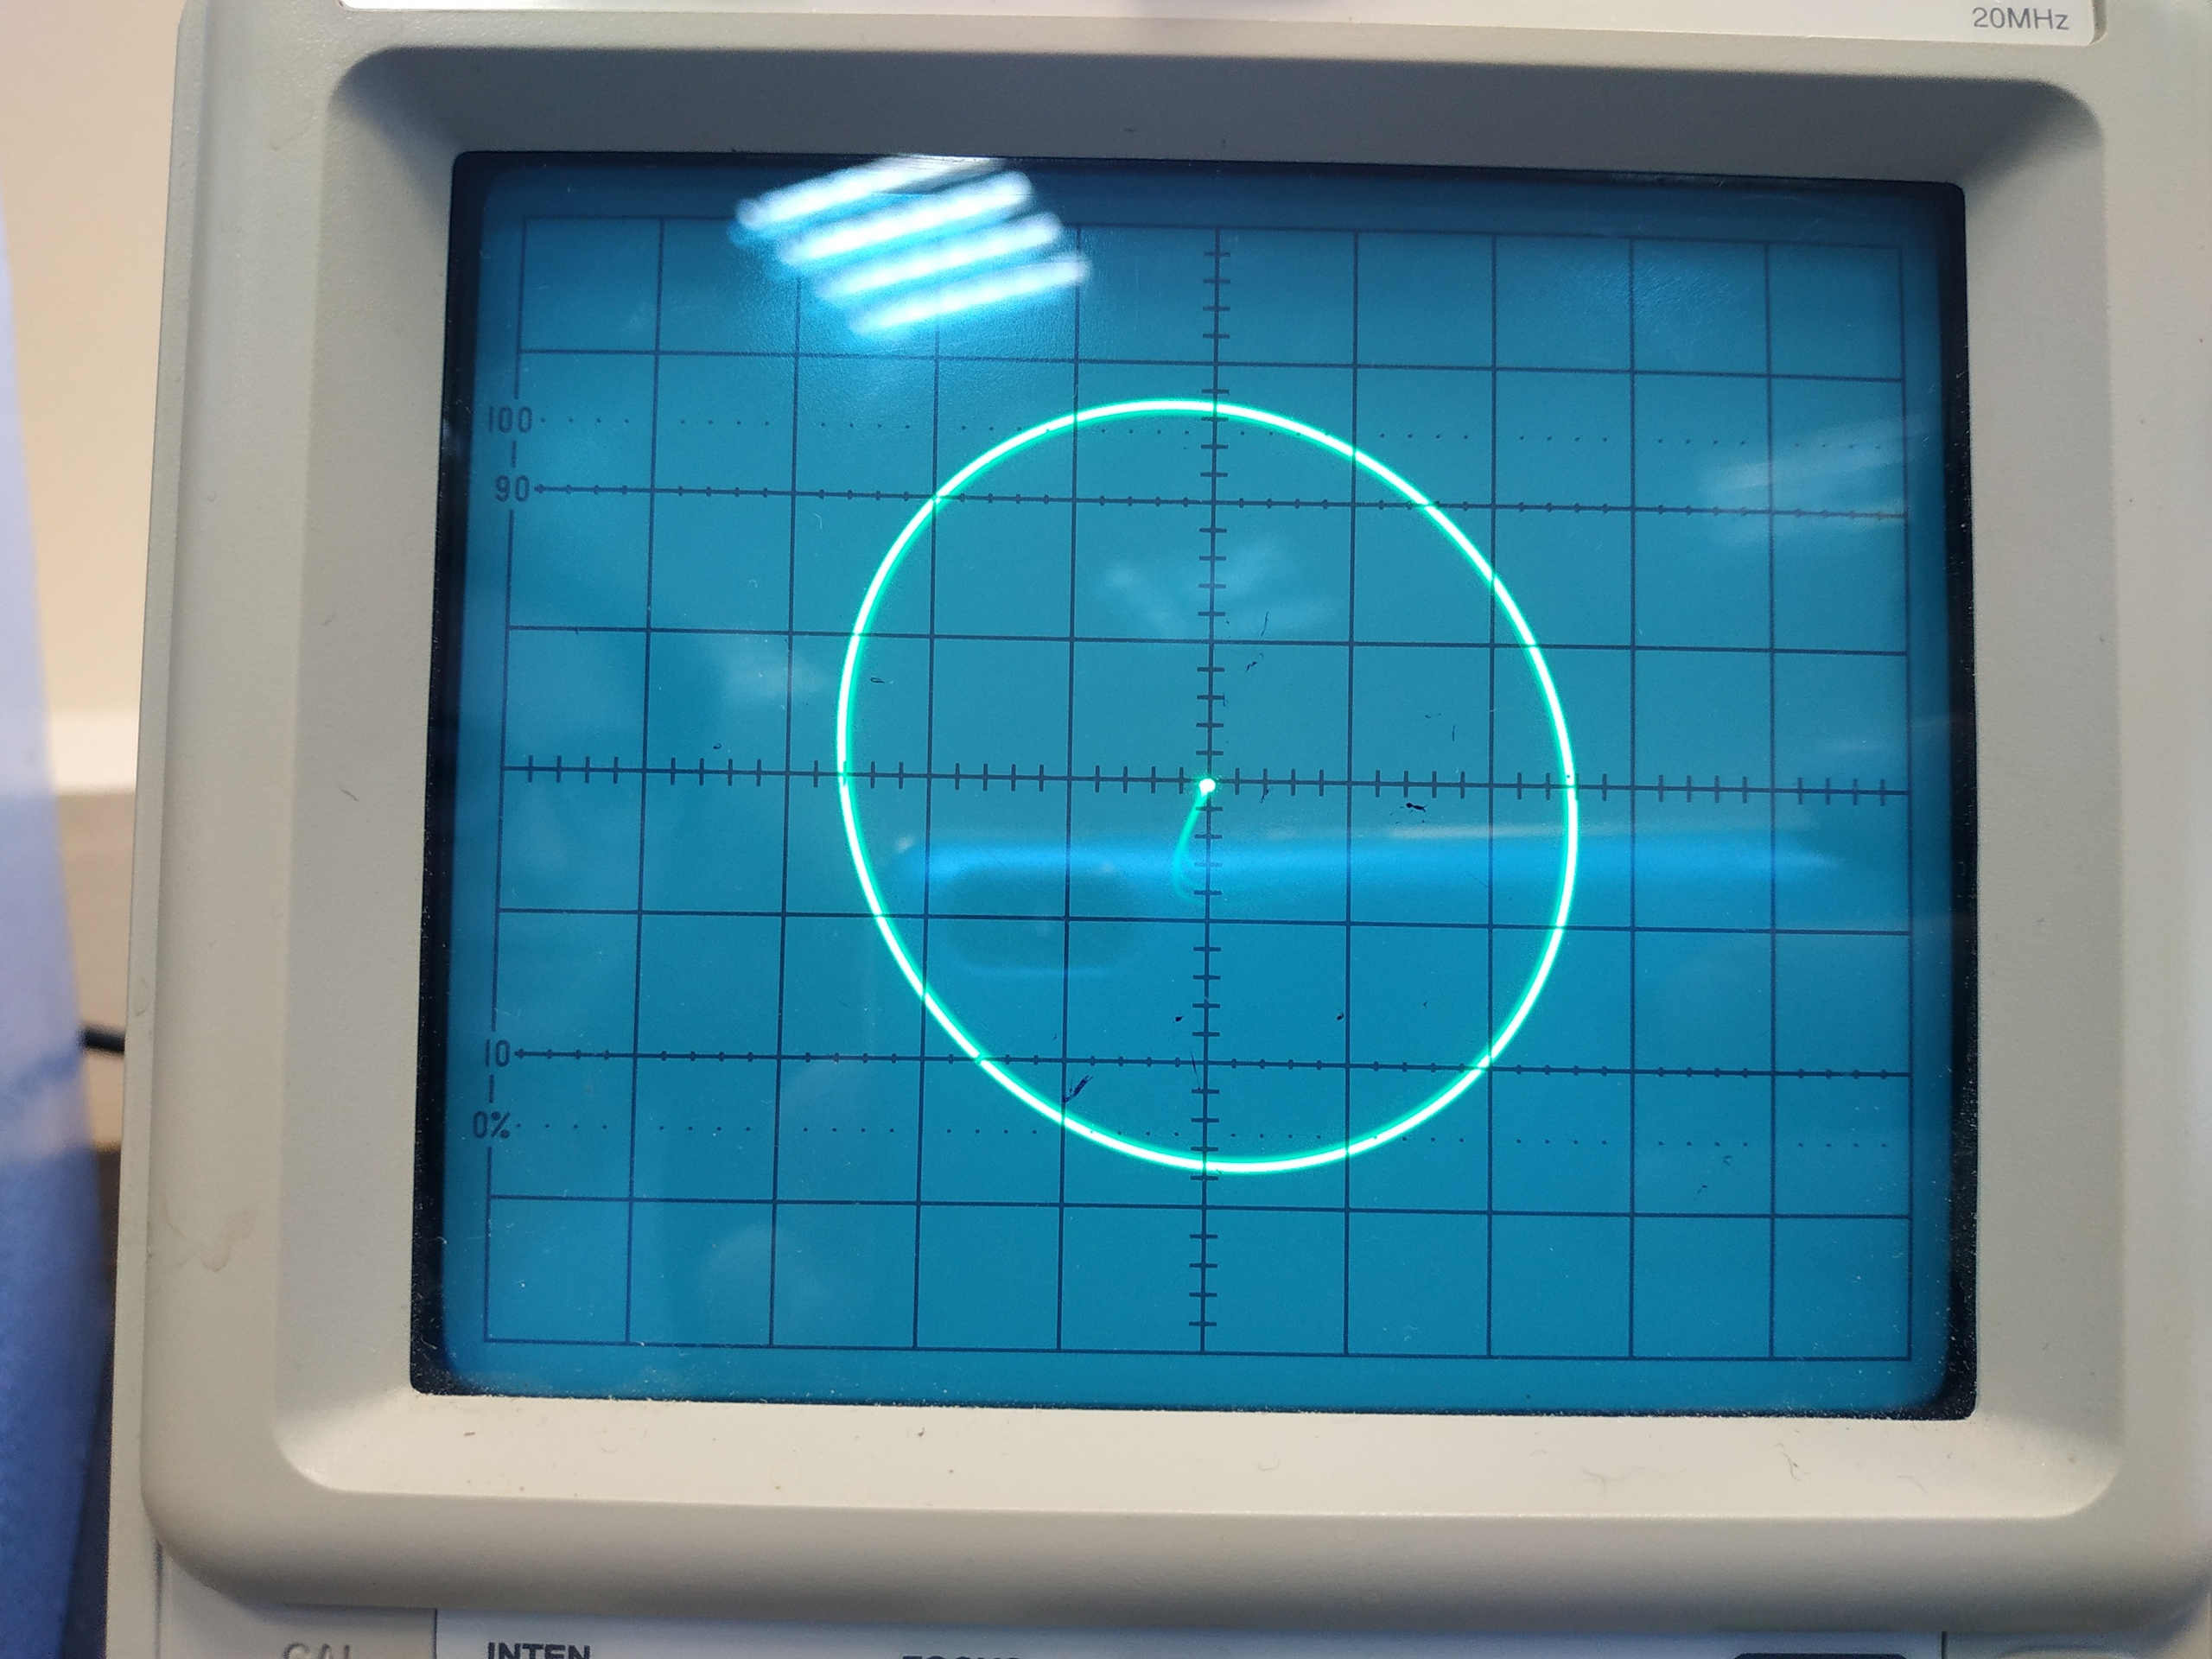
\includegraphics[height=100pt]{img/5.jpg} 
            \vspace{0pt}
            \label{fig:10}
            \captionof{subfigure}{} 
        \end{minipage}
    \begin{minipage}{0.32\linewidth}
        \centering
        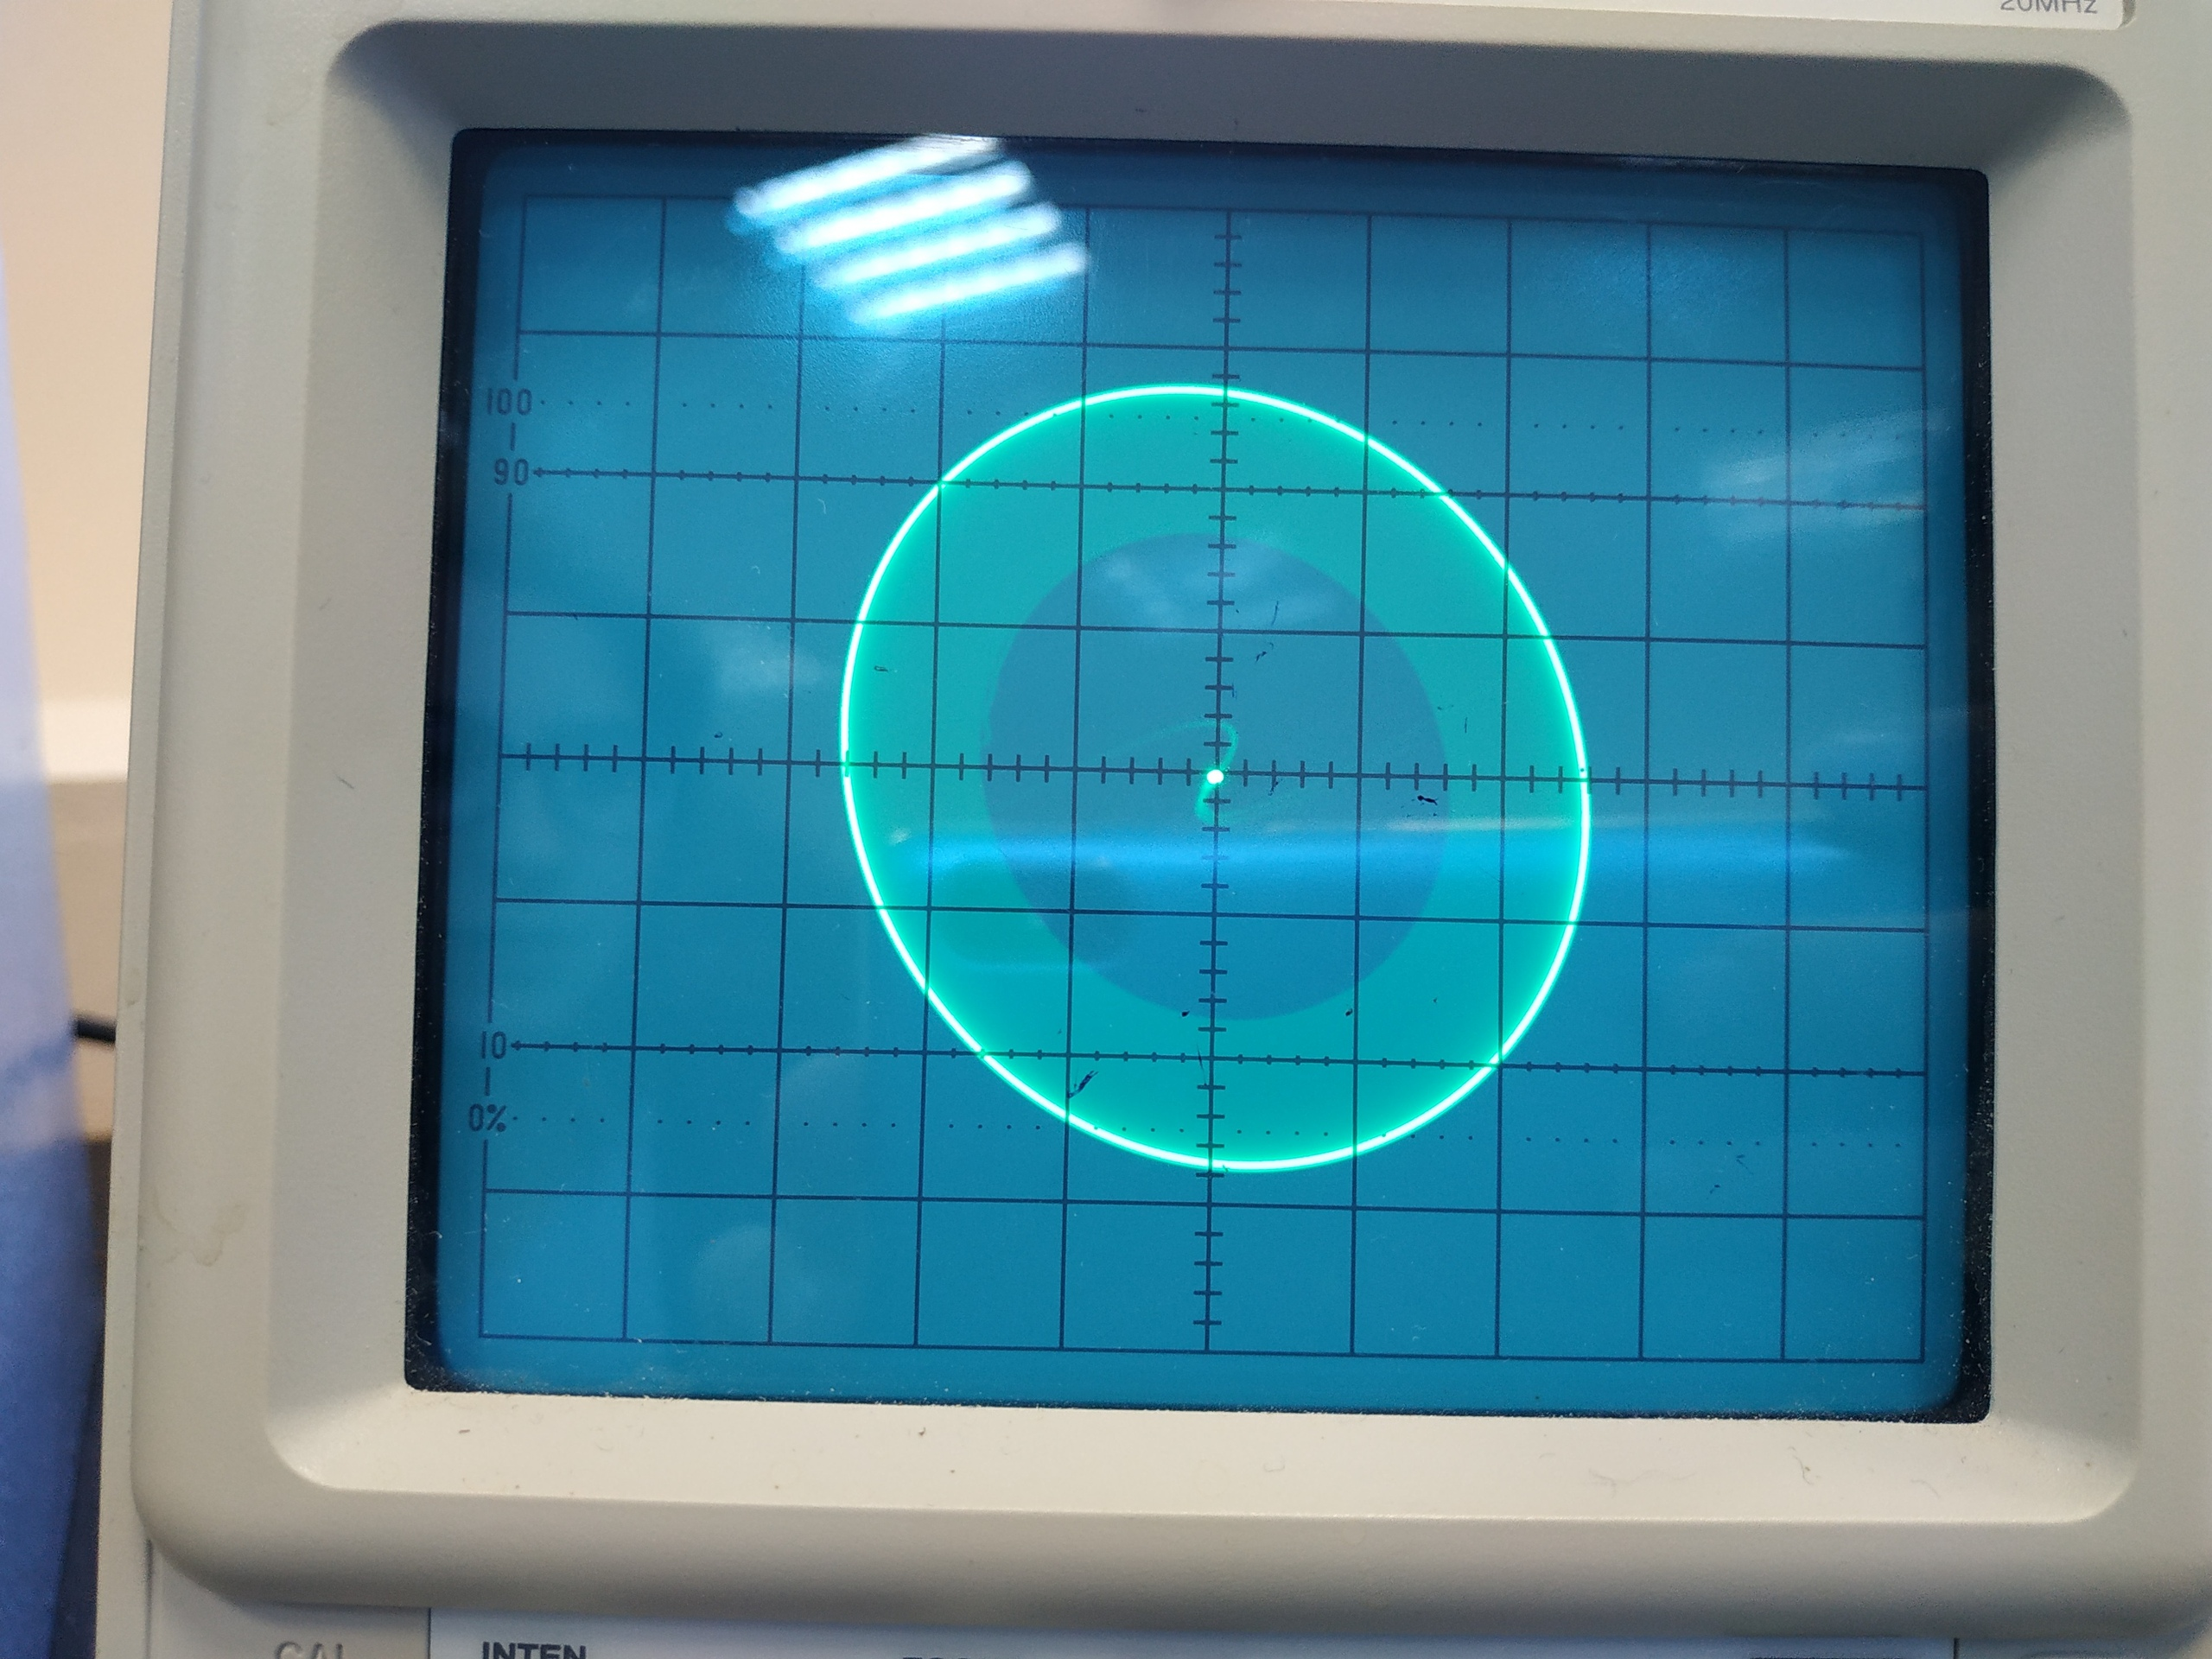
\includegraphics[height=100pt]{img/4.jpg} 
        \vspace{0pt}
        \label{fig:11}
        \captionof{subfigure}{} 
    \end{minipage}
    \begin{minipage}{0.32\linewidth}
        \centering
        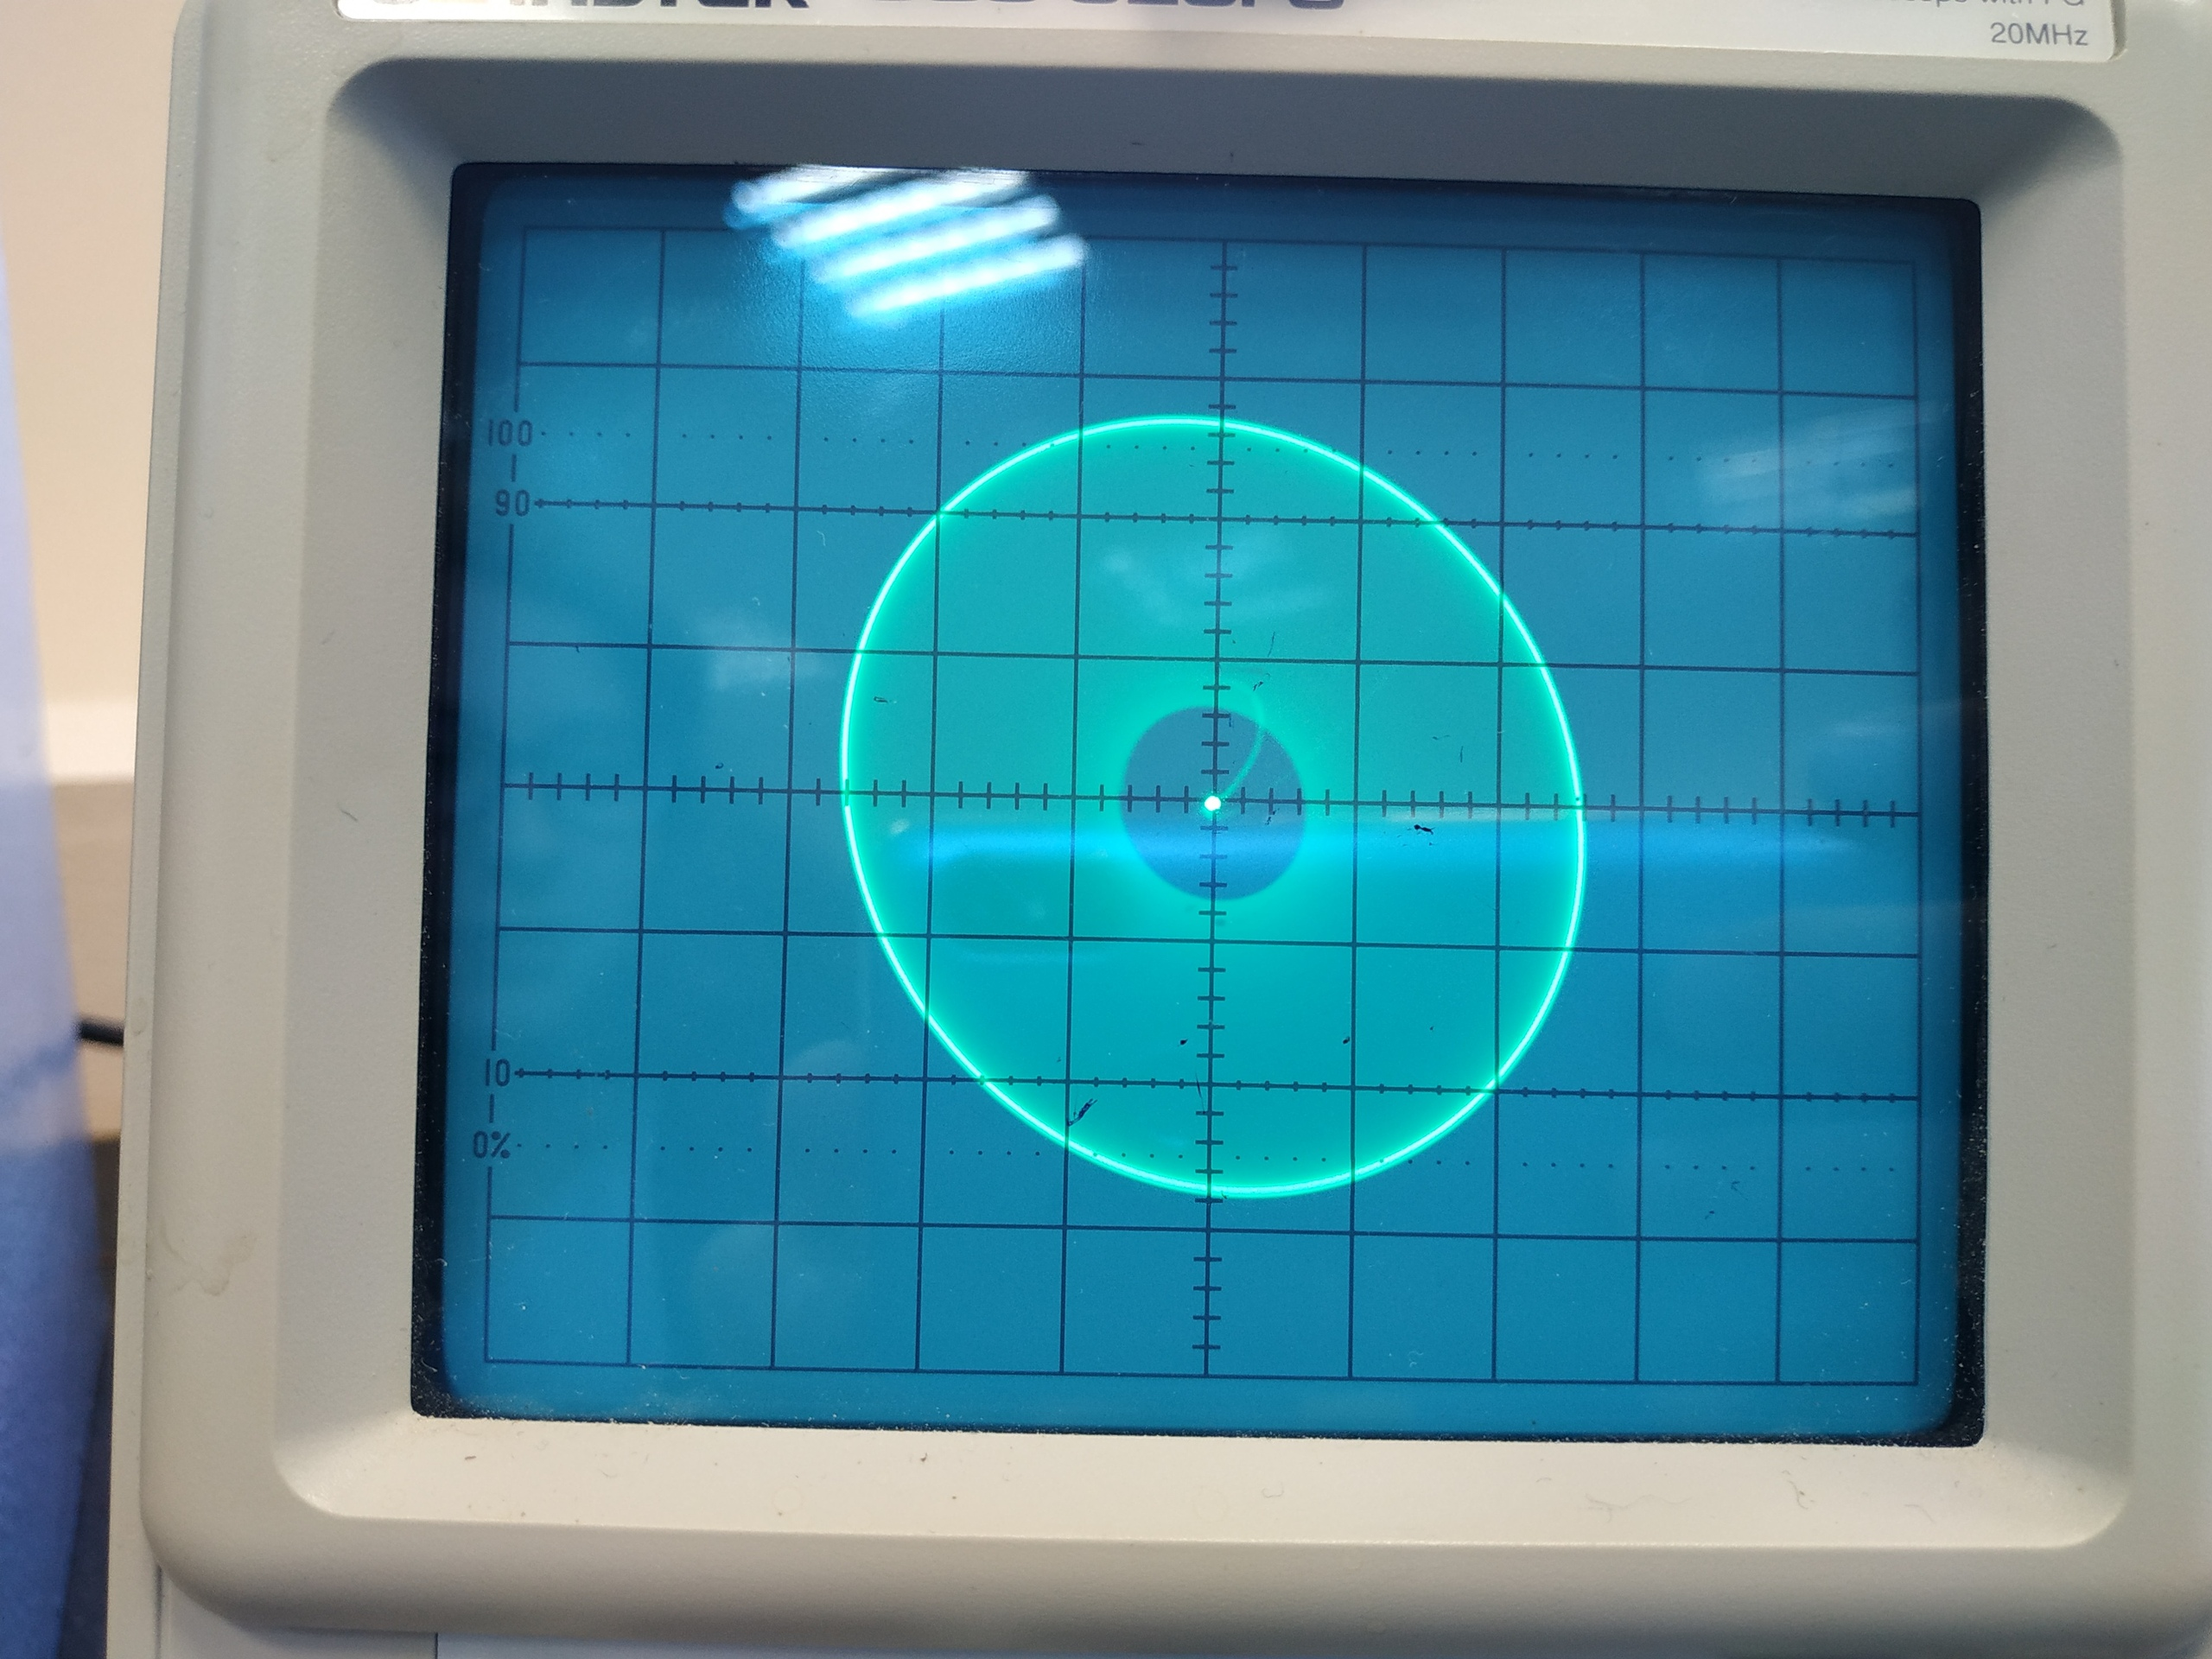
\includegraphics[height=100pt]{img/3.jpg} 
        \vspace{0pt}
        \label{fig:12}
        \captionof{subfigure}{} 
    \end{minipage}
    \caption{Фазовая траектория правее точки бифуркации}
    \vspace{-40pt}
    \end{figure}
\end{center}

Как видно из фазовых траекторий, при значениях $M < M'$ , при любых начальных условиях колебания не устанавливались, а при 
$M > M'$ амплитуда колебаний приходила к одному значению независимо от начальных условий.

Для получения квазипериодического затухающего процесса уменьшалась обратная связь $M$, при этом из развертки и фазовой траектории, приведенной на рис. 17, 
был получен декремент затухания для двух значений $M$, лежащих левее точки бифуркации.

\begin{table}[H]
    \centering
    \begin{tabular}{@{}|c|c|c|@{}}
    \hline
        $M, y.e$     & -10 & -25 \\ \hline
    $\delta$ & 0.63 & 0.56 \\ \hline
    \end{tabular}
\end{table}

Апериодического процесса достичь не удалось, в связи со слишком маленьким максимальным сопротивлением установки. Достигнутый процесс приведен на рис. 18
\begin{center}
    \begin{figure}[H]
    \begin{minipage}{.49\linewidth}
        \vspace{-10pt}
        \centering
        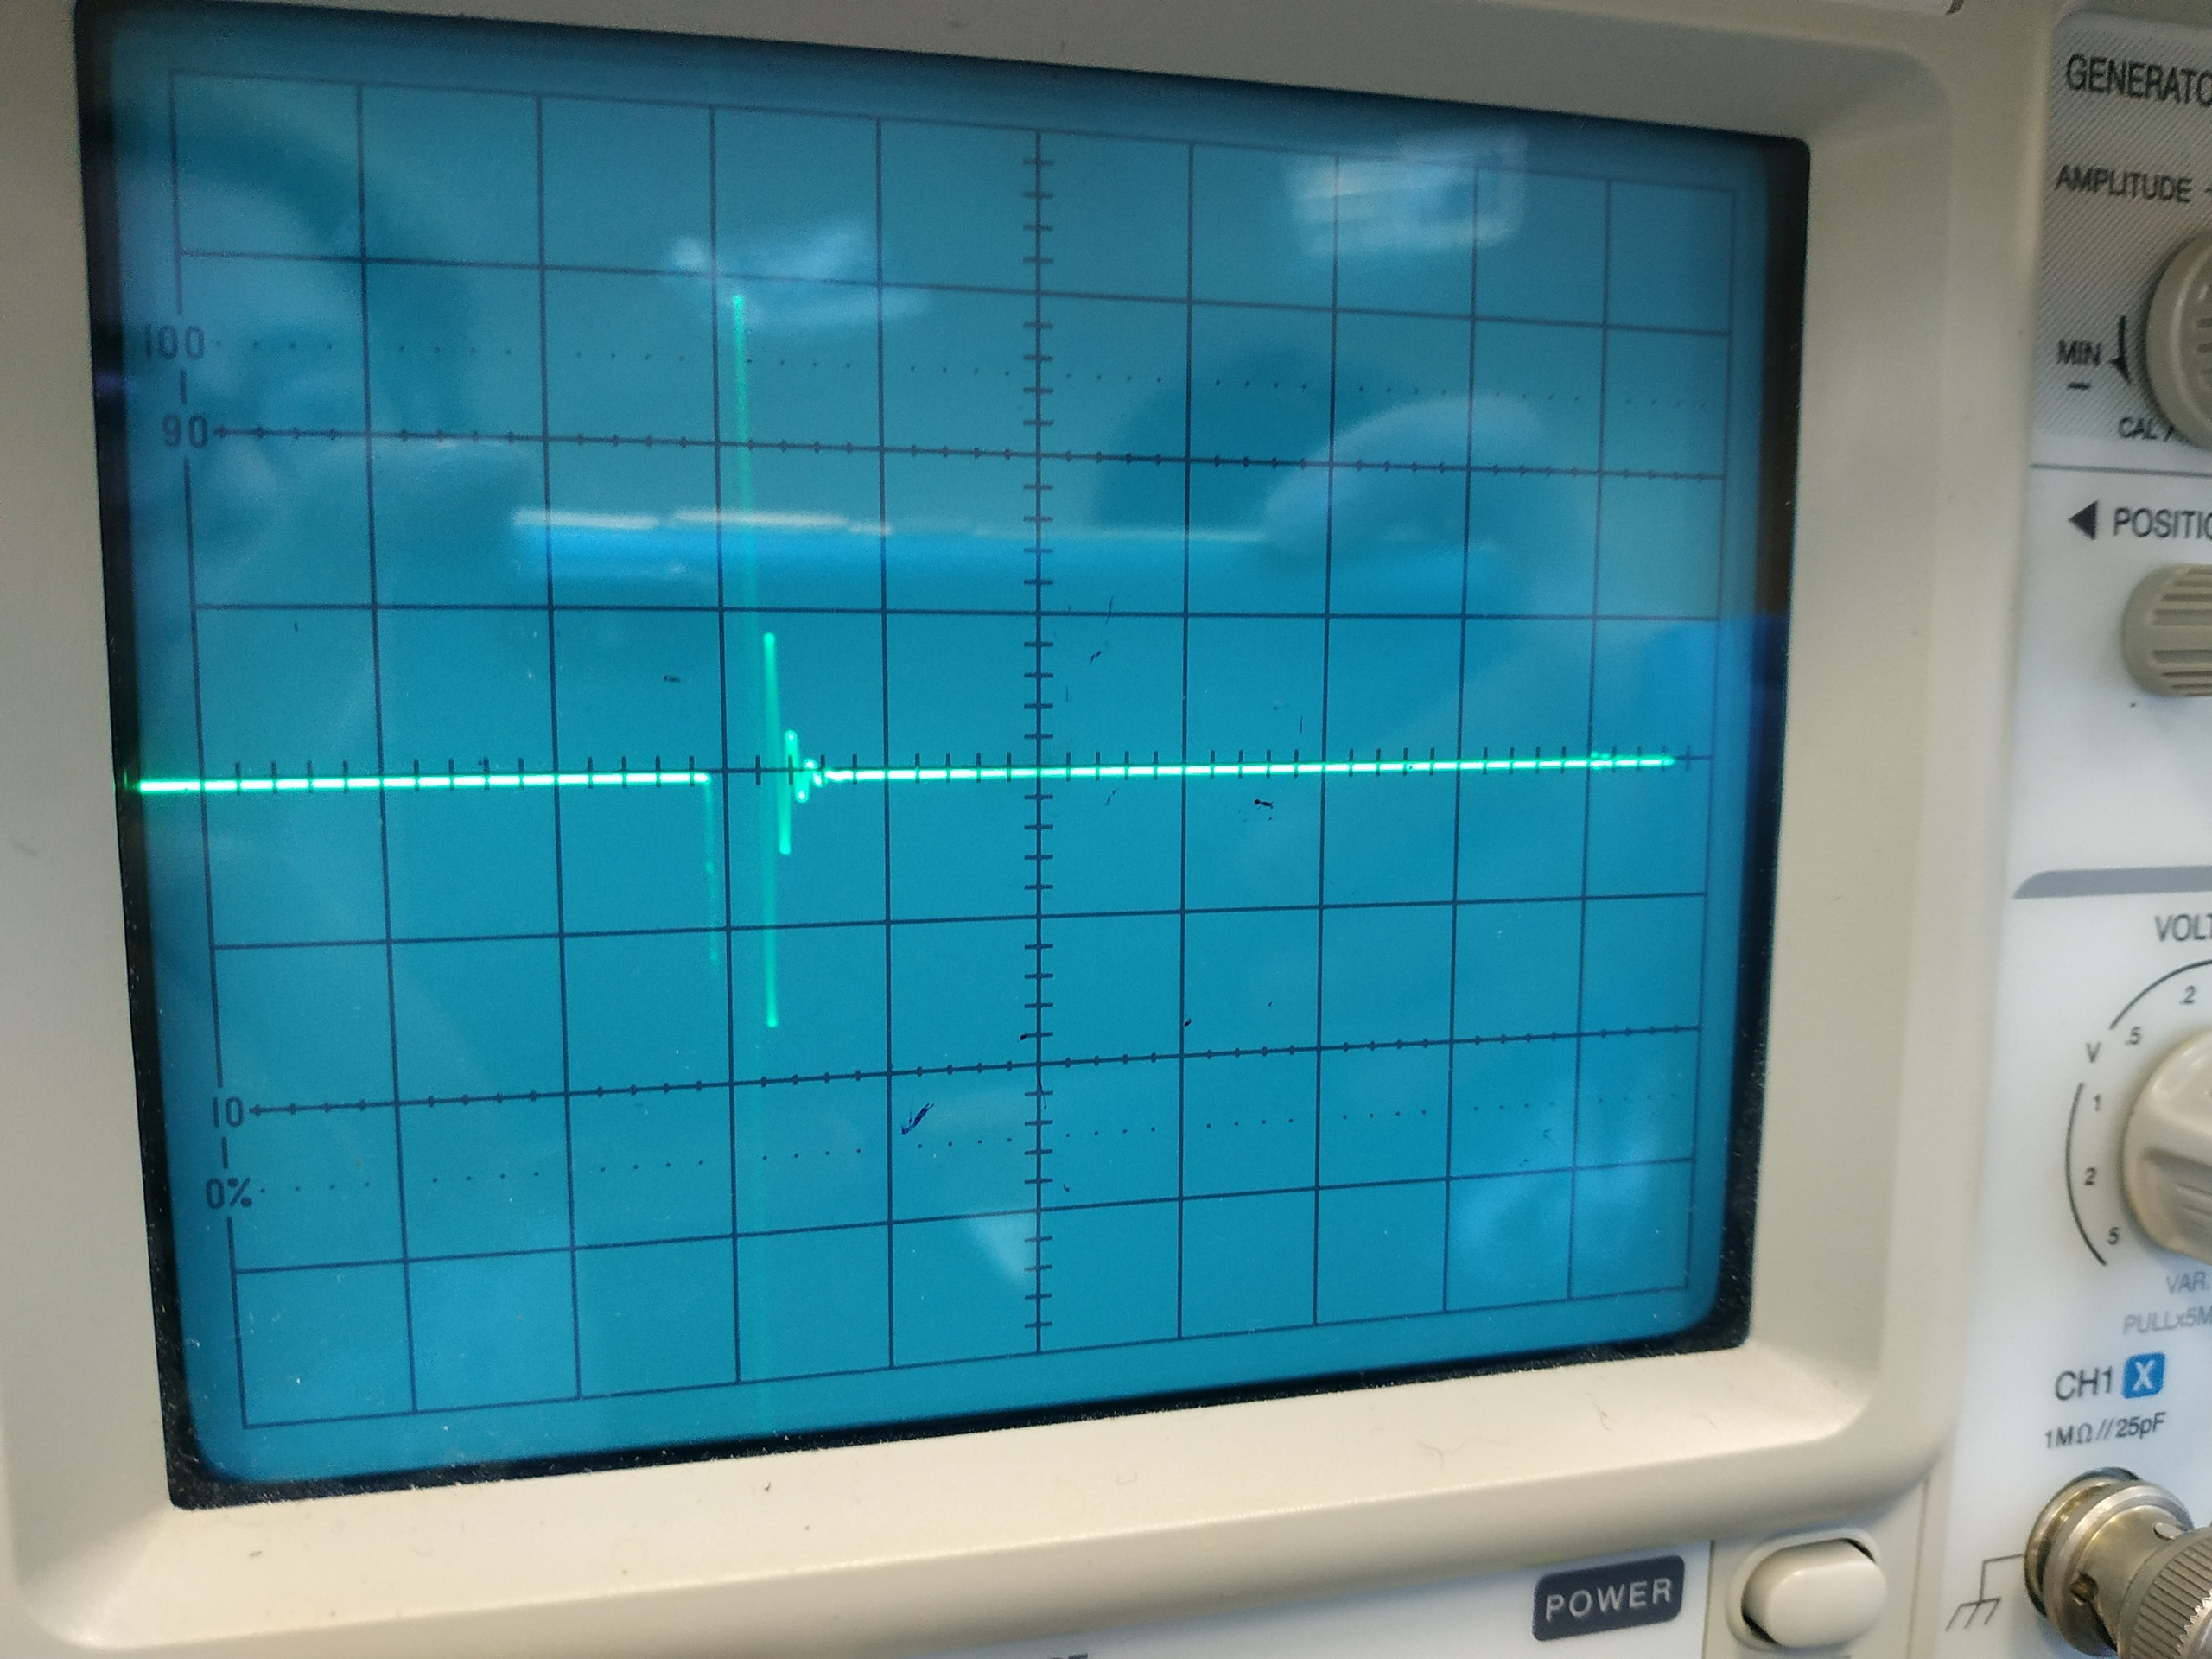
\includegraphics[height=120pt]{img/12.jpg} 
        \vspace{0pt}
        \label{fig:10}
        \captionof{figure}{} 
        \vspace{-20pt}
    \end{minipage}
    \begin{minipage}{.49\linewidth}
        \vspace{-10pt}
        \centering
        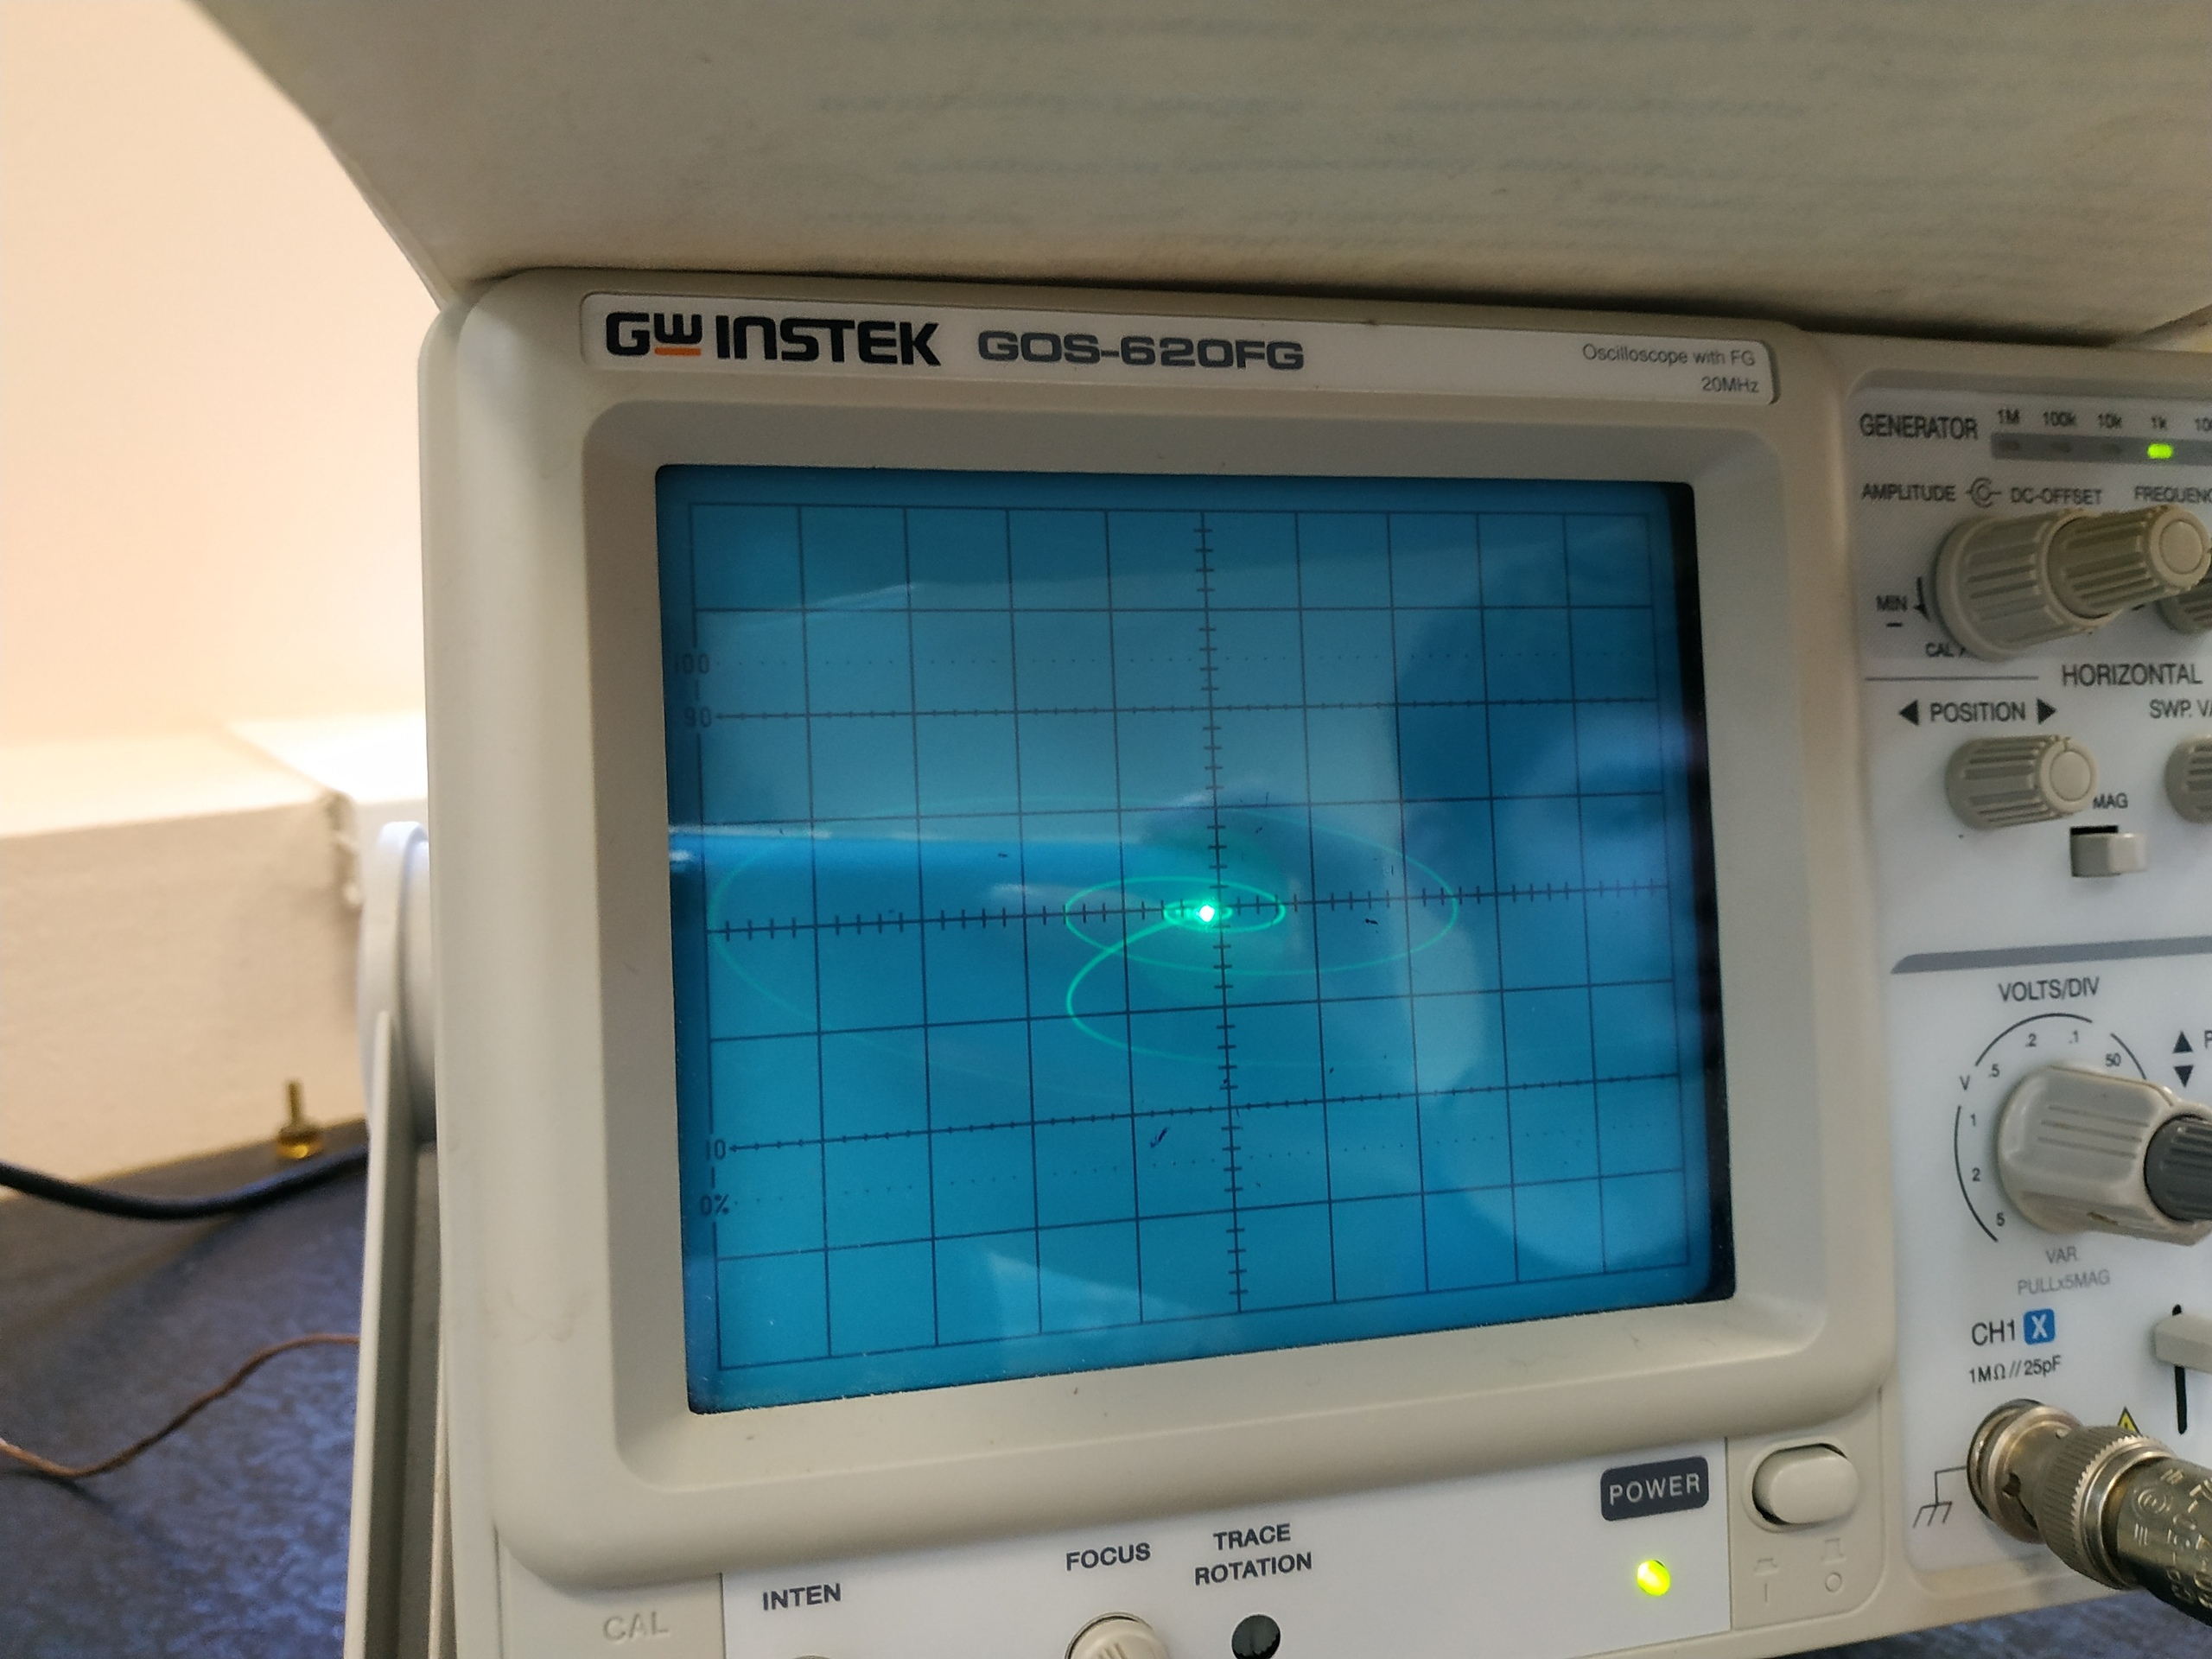
\includegraphics[height=120pt]{img/13.jpg} 
        \vspace{0pt}
        \label{fig:10}
        \captionof{figure}{} 
        \vspace{-20pt}
    \end{minipage}
    \end{figure}
\end{center} 
\subsection{Жесткий режим генератора}

Для определения жесткого режима при выставленном $E_0$ менялось значение $M$. Признаком жесткого режима было
 резкое увеличение амплитуды после преодоления некоторого значения $M''$.
Снятая бифуркационная диаграмма приведена на рис. 19.
\begin{center}
    \begin{figure}[H]
        \vspace{-10pt}
            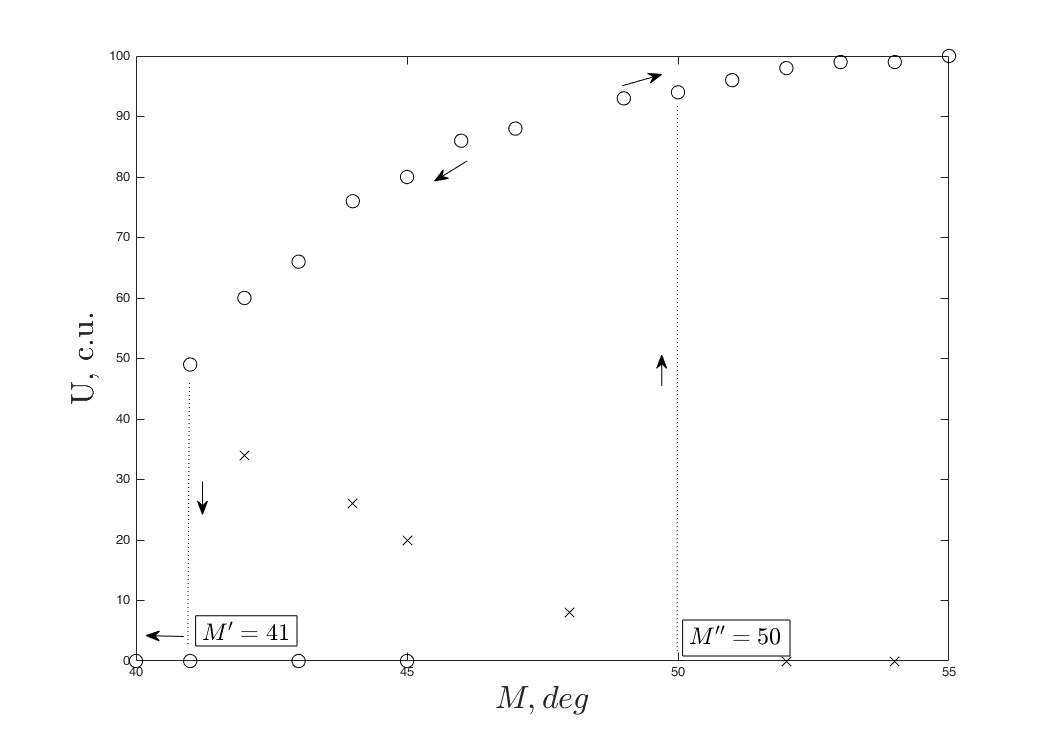
\includegraphics[width=\linewidth]{graph/g2.png} 
            \vspace{-10pt}
            \label{fig:10}
            \captionof{figure}{Бифуркационная диаграмма для жесткого режима генератора} 
            \vspace{-40pt}
    \end{figure}
\end{center} 
Для нахождения неустойчивых значений амплитуды включался прерыватель, и по фазовой траектории определялась устойчивость точки.
Признаком попадания на неустойчивую точку было наблюдение двух картин одновременно, т.е. колебания как устанавливались, так и затухали.
 Пример такой фазовой траектории приведен на рис. 21a.


 Из бифуркационной диаграммы были получены значения для $M',M''$ , соответствующие параметрам $\sigma'$ и $\sigma''$.
$$M'=  41 \pm 1 y.e.$$ $$M''= 50 \pm 1 y.e.$$
Фазовые траектории для жесткого режима приведены на рис. 20 - рис. 22.


\begin{center}
    \begin{figure}[H]
        \begin{minipage}{0.32\linewidth}
            \centering
            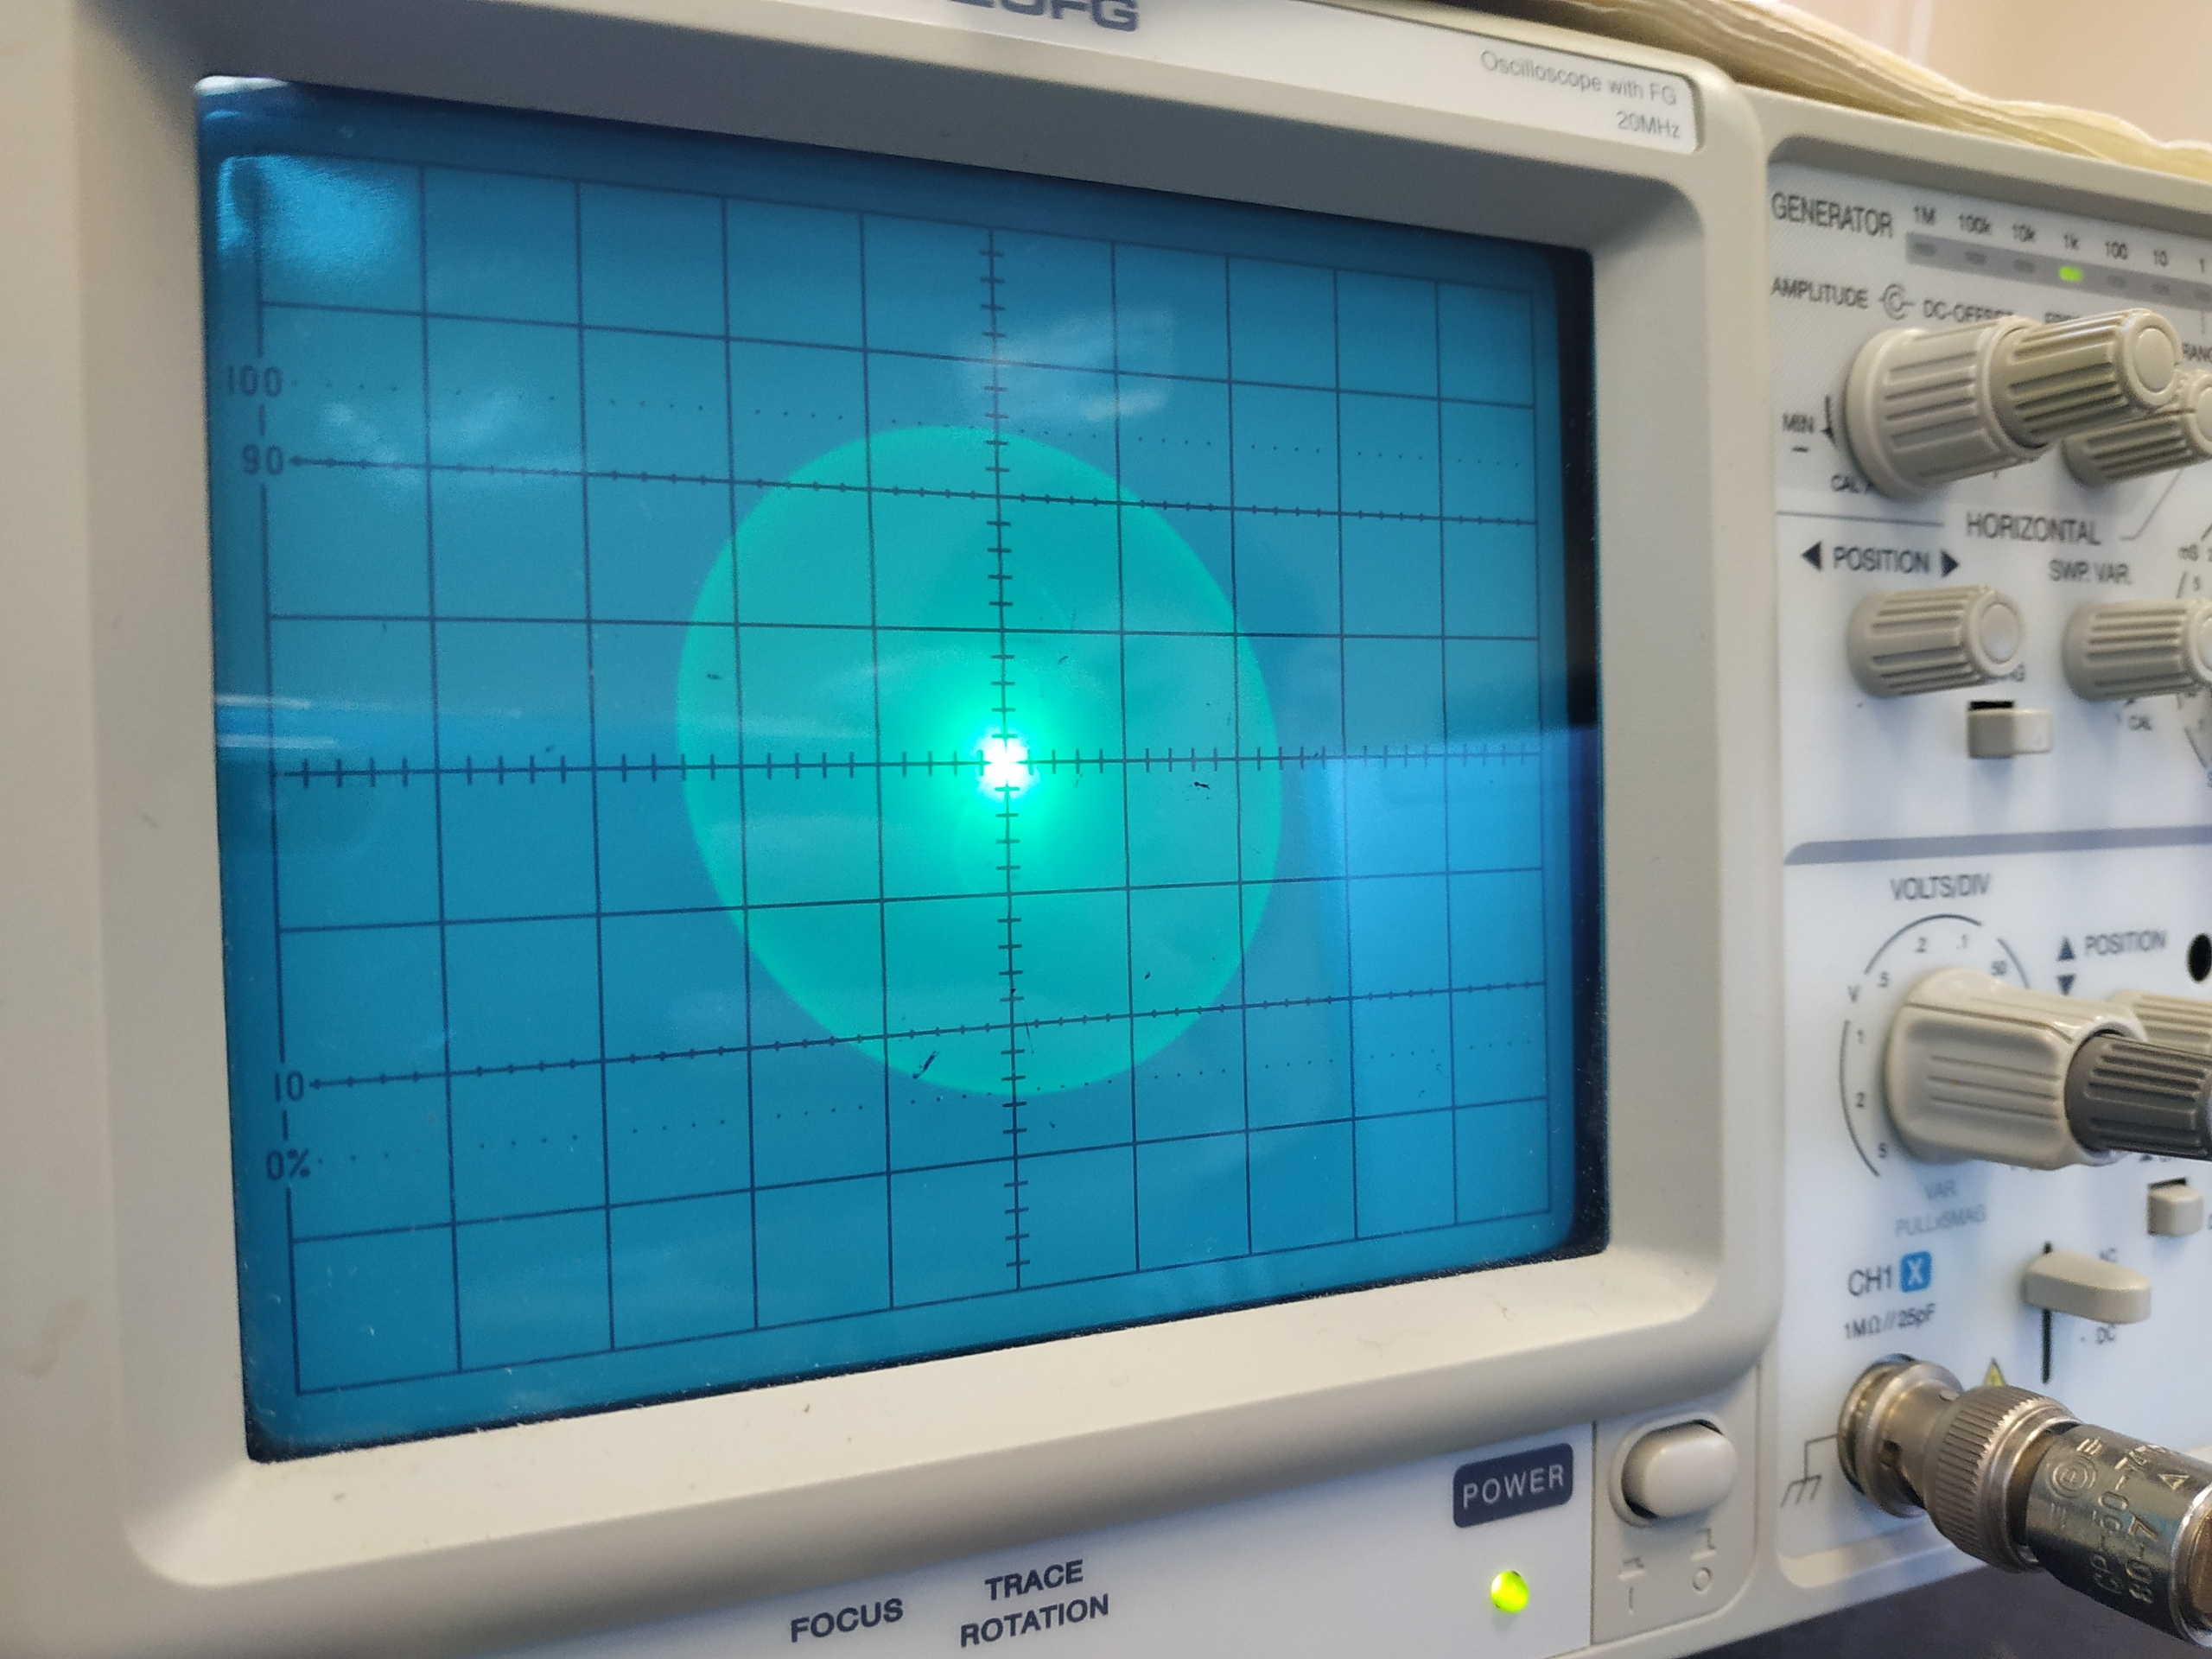
\includegraphics[height=100pt]{img/1.jpg} 
            \vspace{0pt}
            \label{fig:10}
            \captionof{subfigure}{} 
        \end{minipage}
        \begin{minipage}{0.32\linewidth}
            \centering
            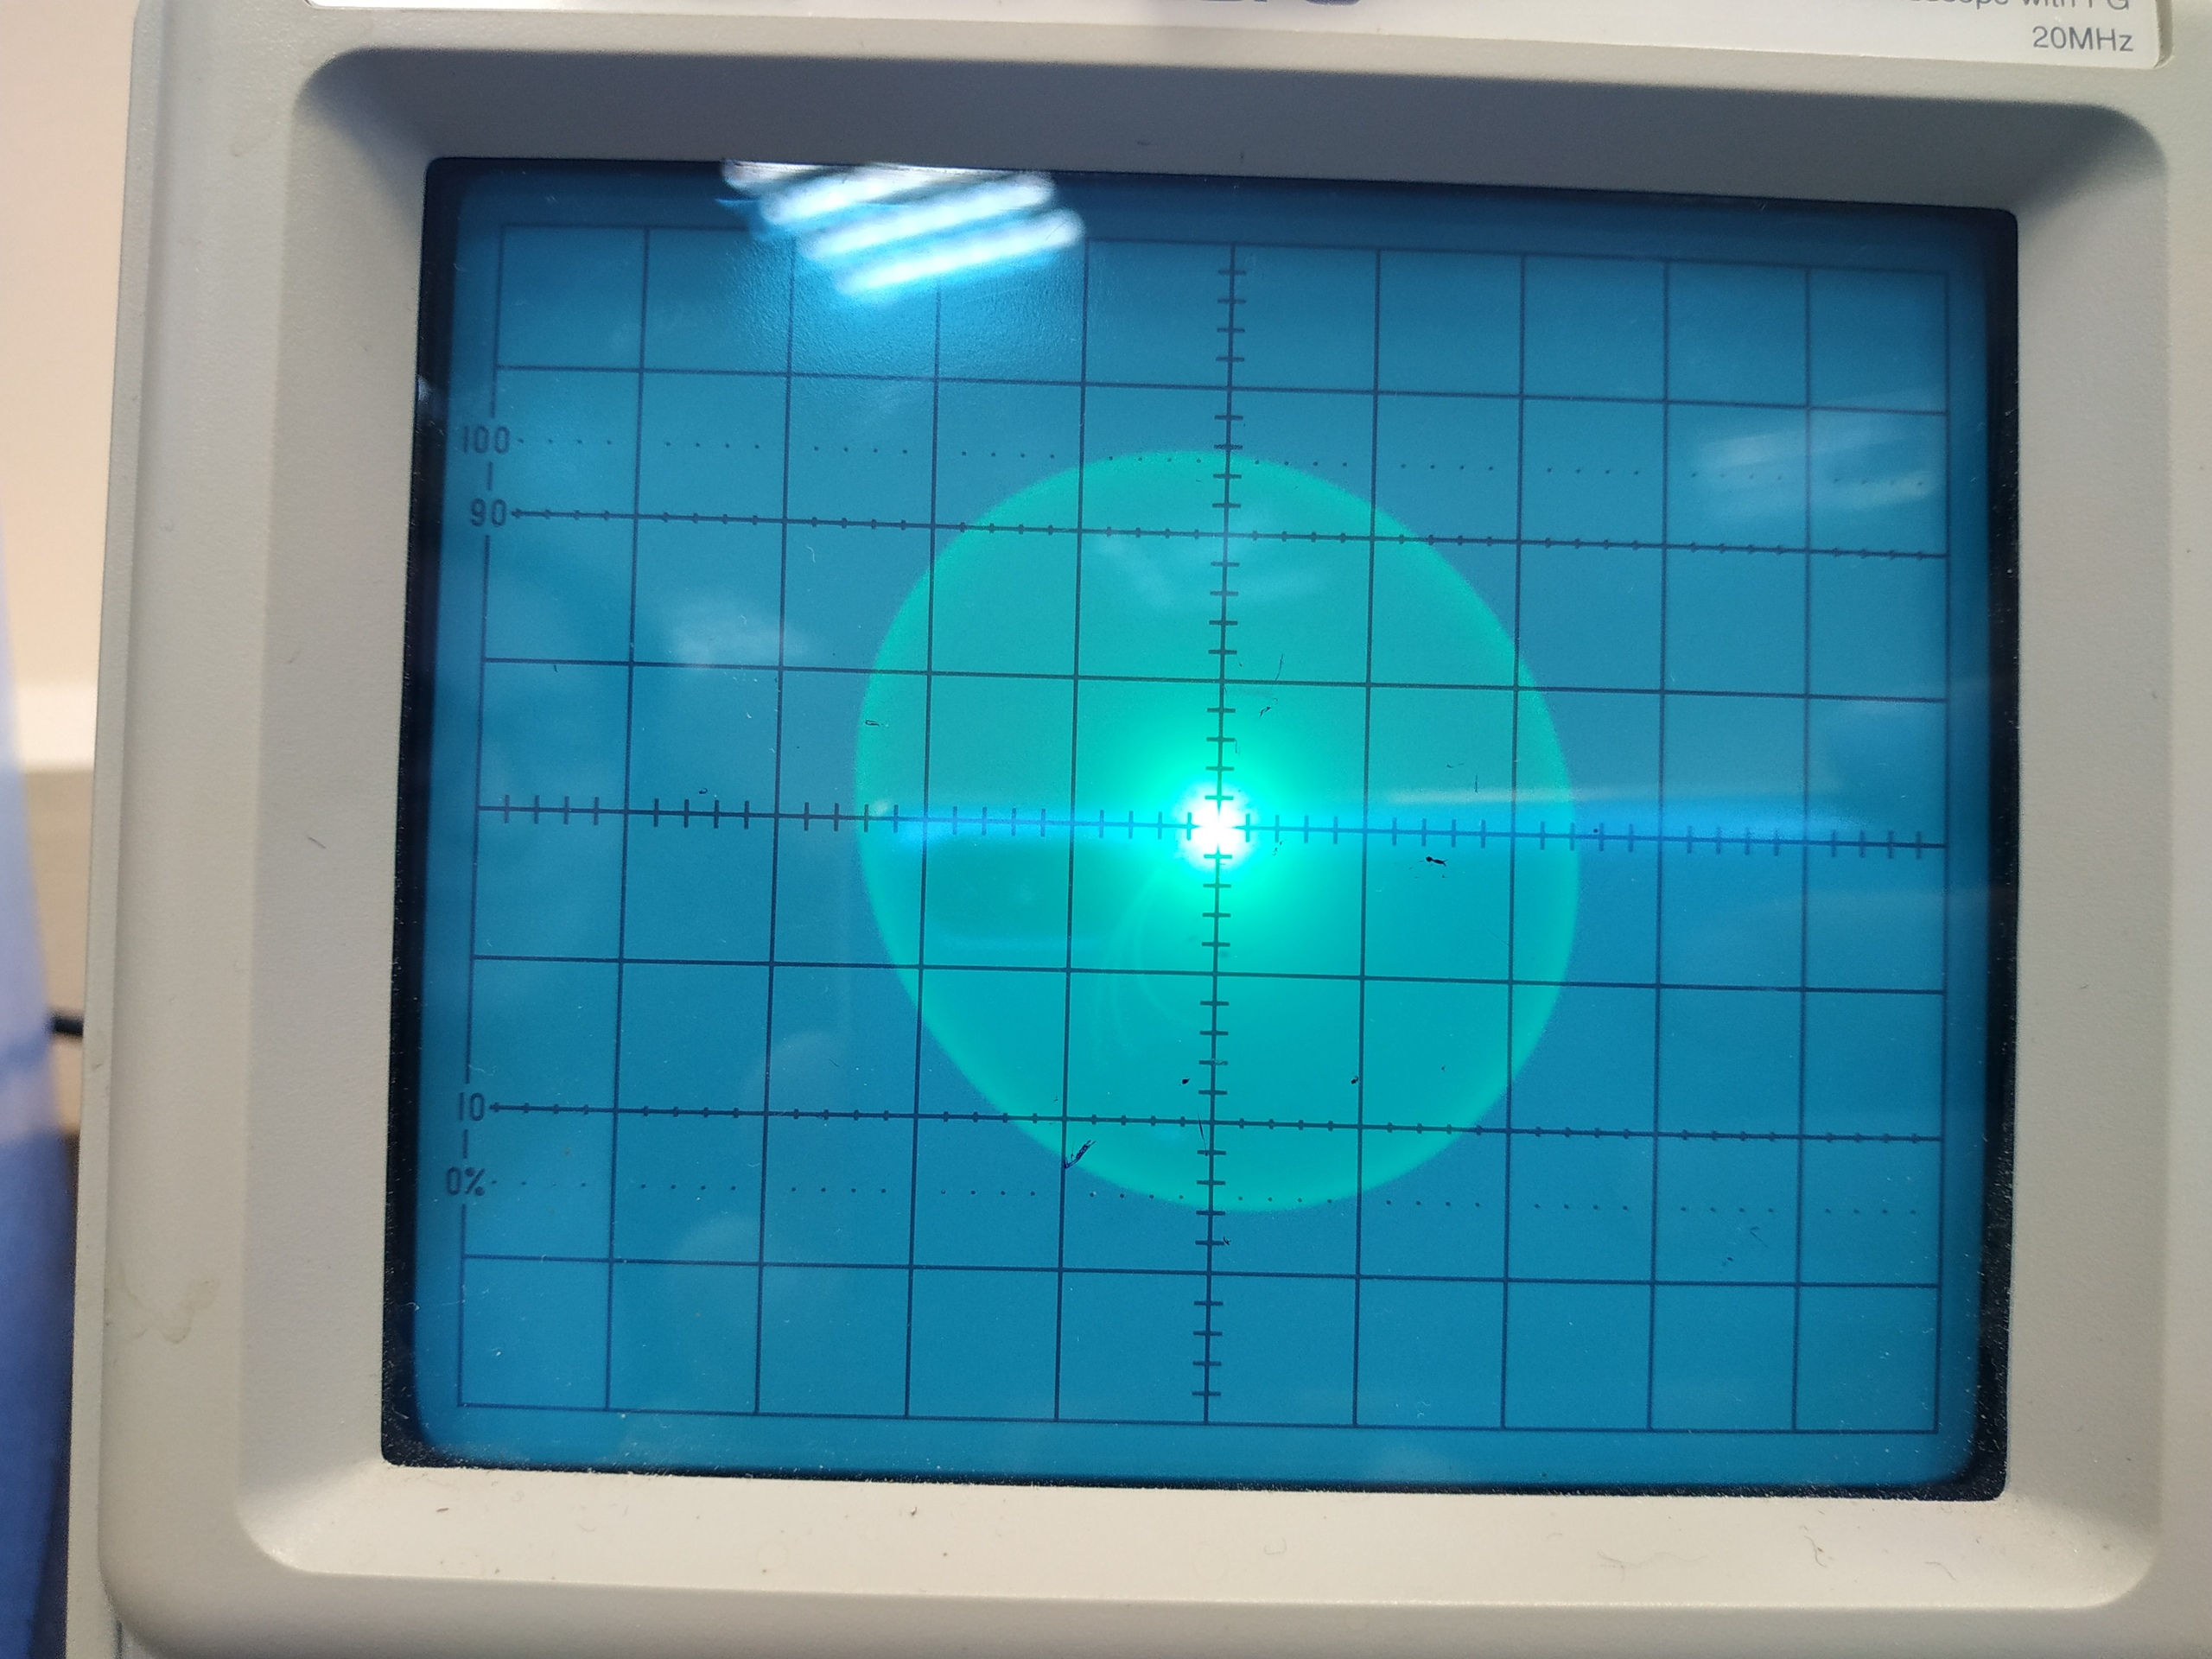
\includegraphics[height=100pt]{img/2.jpg} 
            \vspace{0pt}
            \label{fig:11}
            \captionof{subfigure}{} 
        \end{minipage}
        \begin{minipage}{0.32\linewidth}
            \centering
            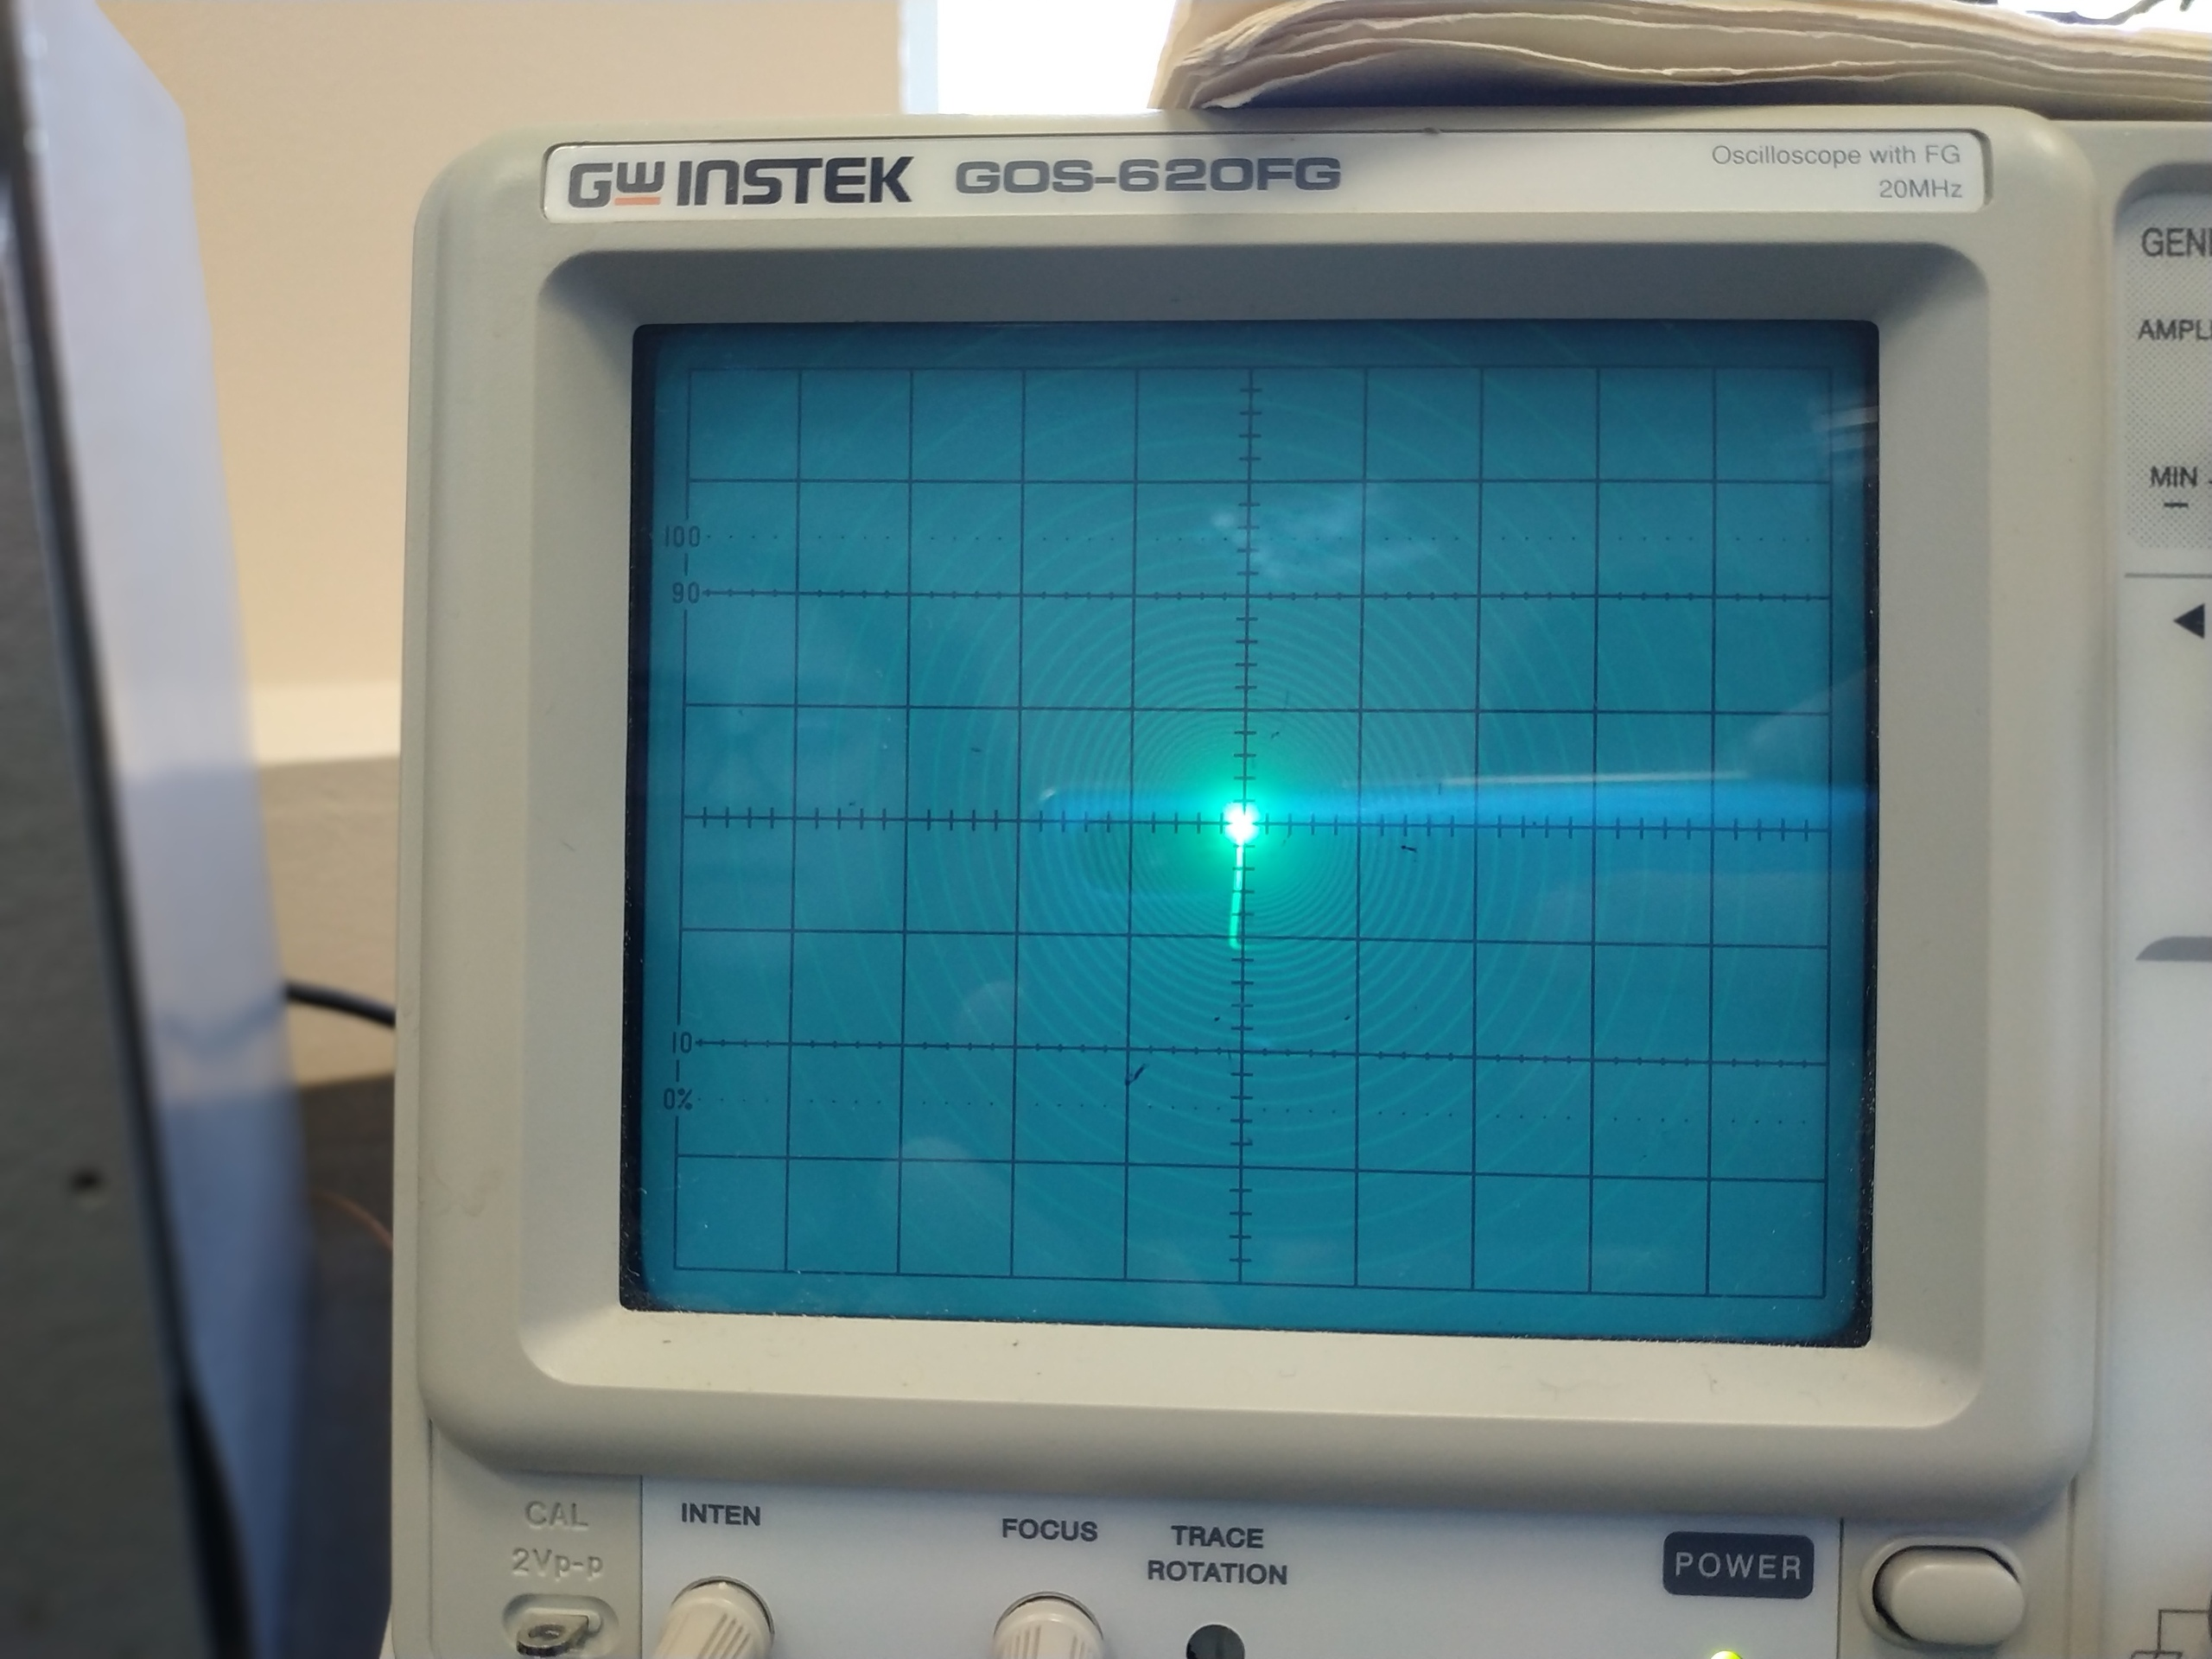
\includegraphics[height=100pt]{img/9.jpg} 
            \vspace{0pt}
            \label{fig:12}
            \captionof{subfigure}{} 
        \end{minipage}
    \caption{Фазовая траектория для $M < M'$}
    \vspace{-40pt}
    \end{figure}
\end{center} 
\begin{center}
    \begin{figure}[H]
        % \begin{minipage}{0.32\linewidth}
        %     \centering
        %     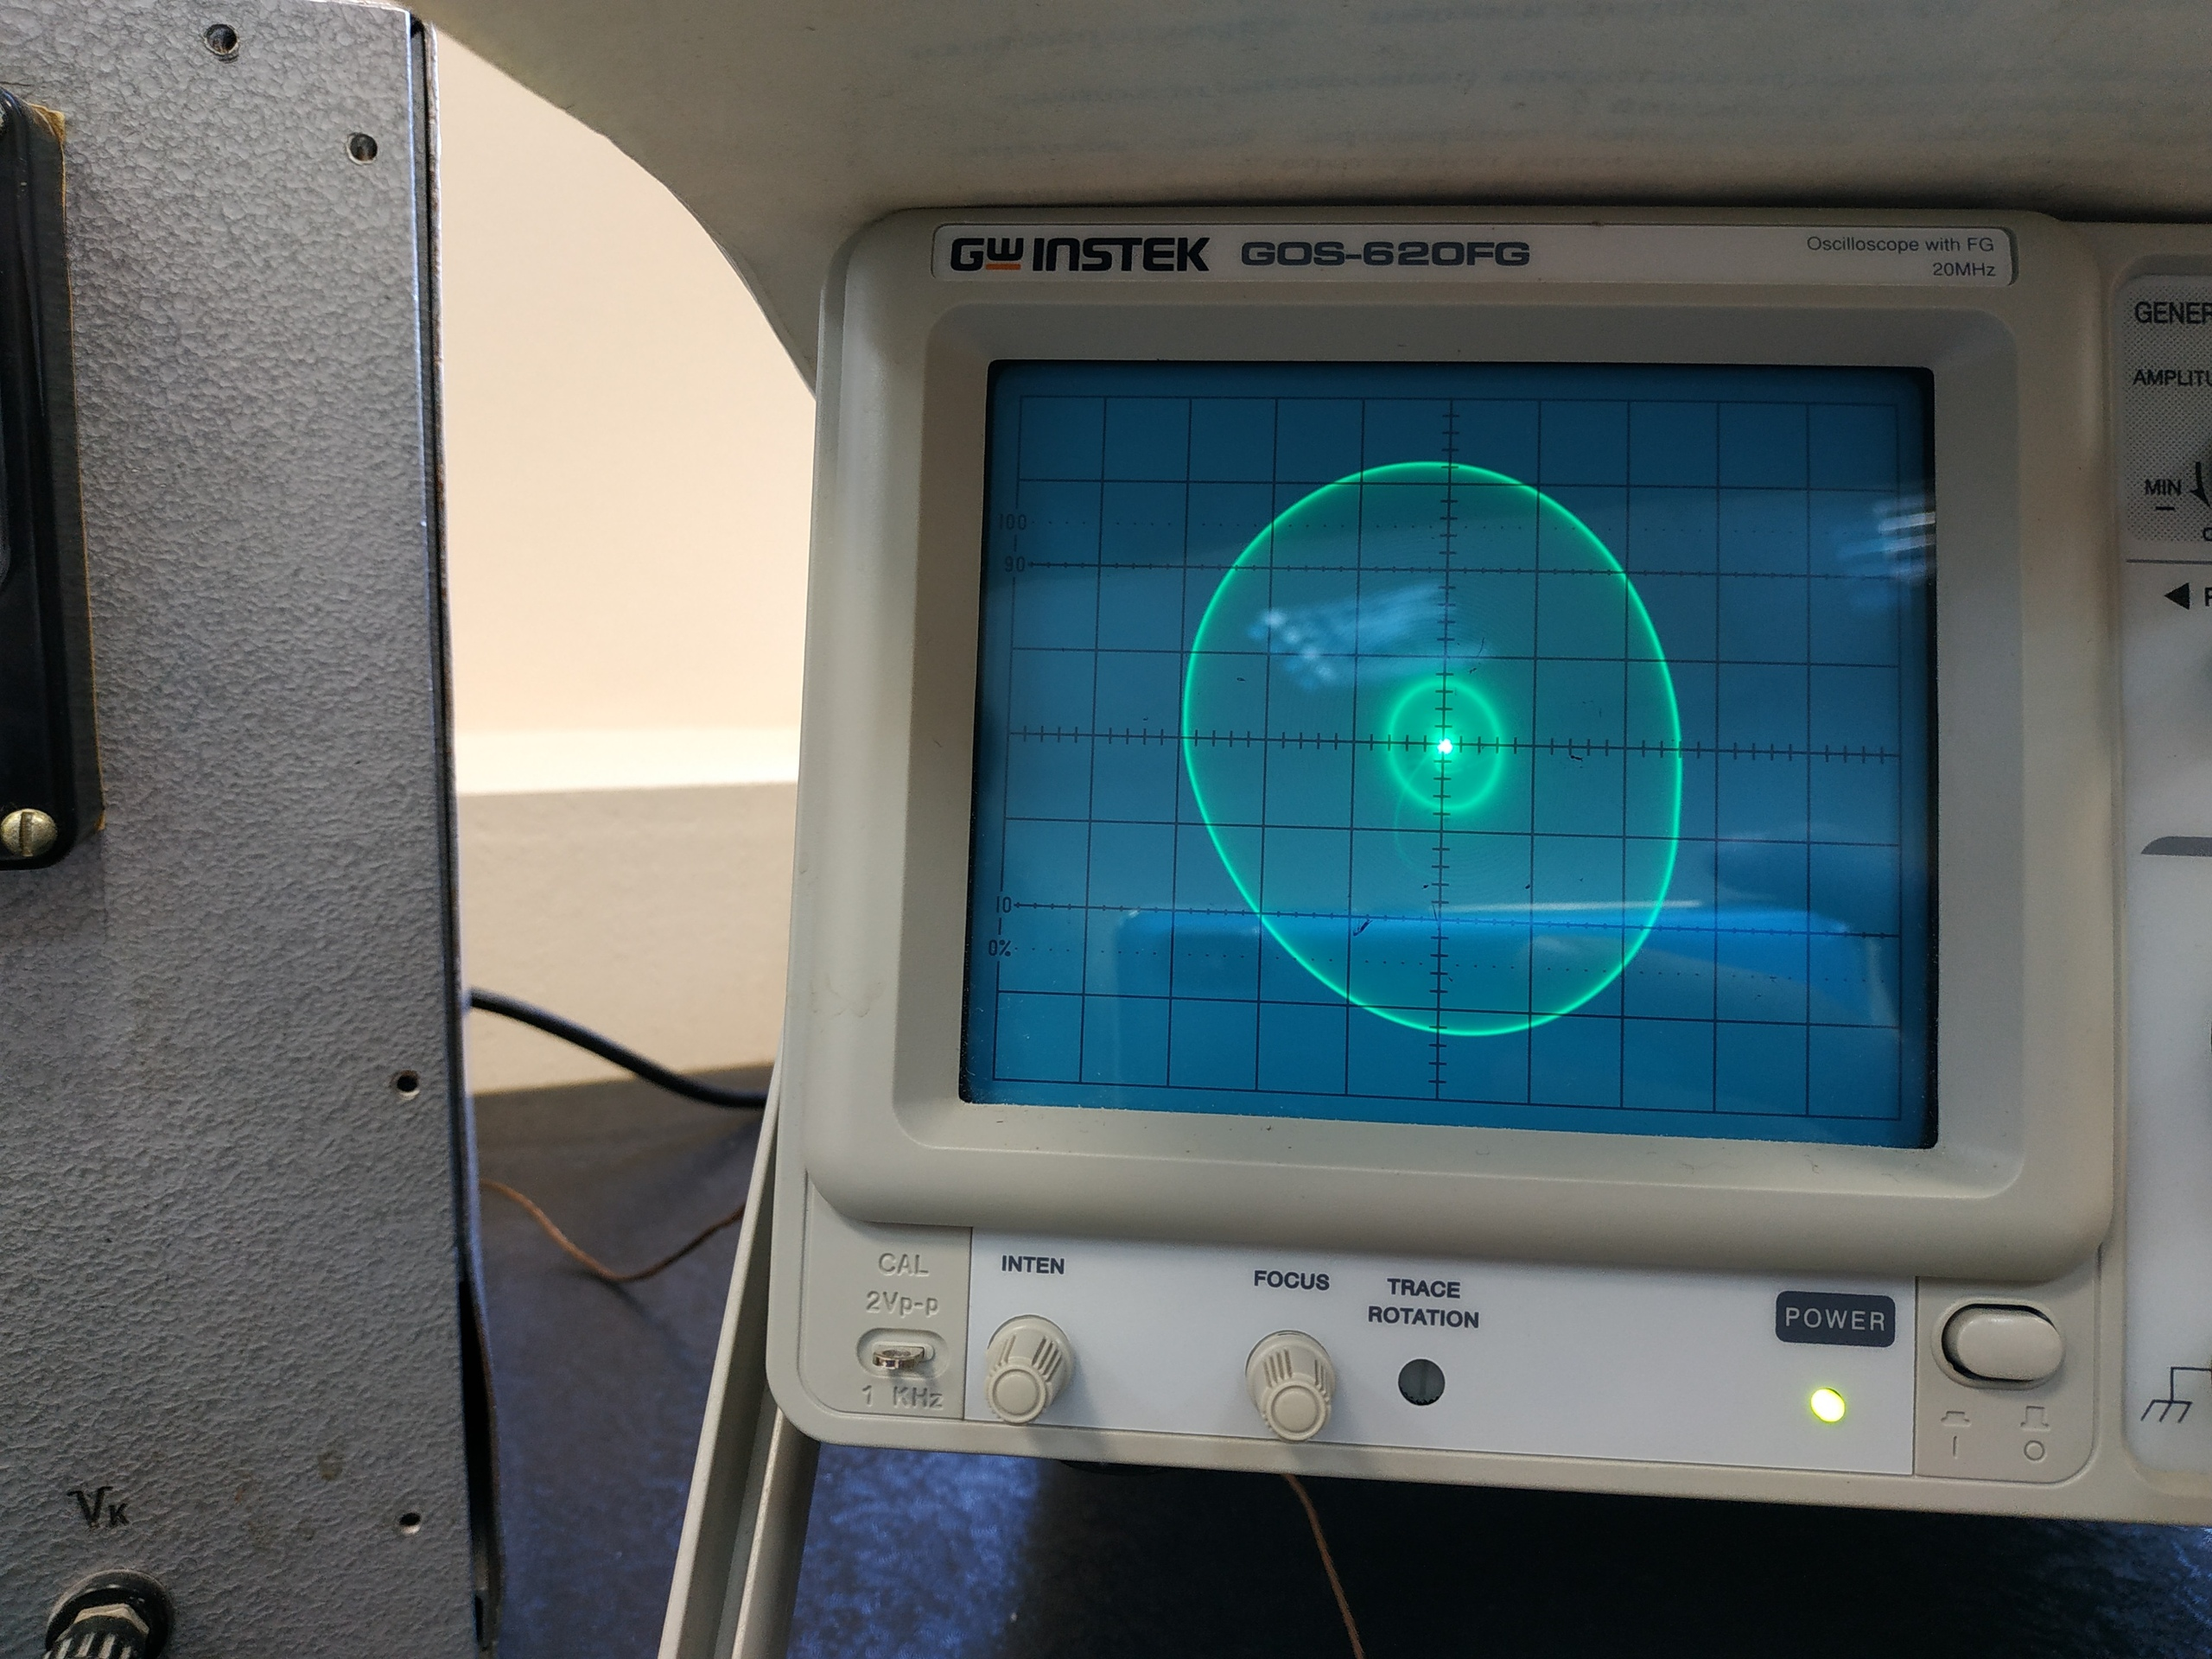
\includegraphics[height=100pt]{img/15.jpg} 
        %     \vspace{0pt}
        %     \label{fig:10}
        %     \captionof{subfigure}{} 
        % \end{minipage}
        \begin{minipage}{0.49\linewidth}
            \centering
            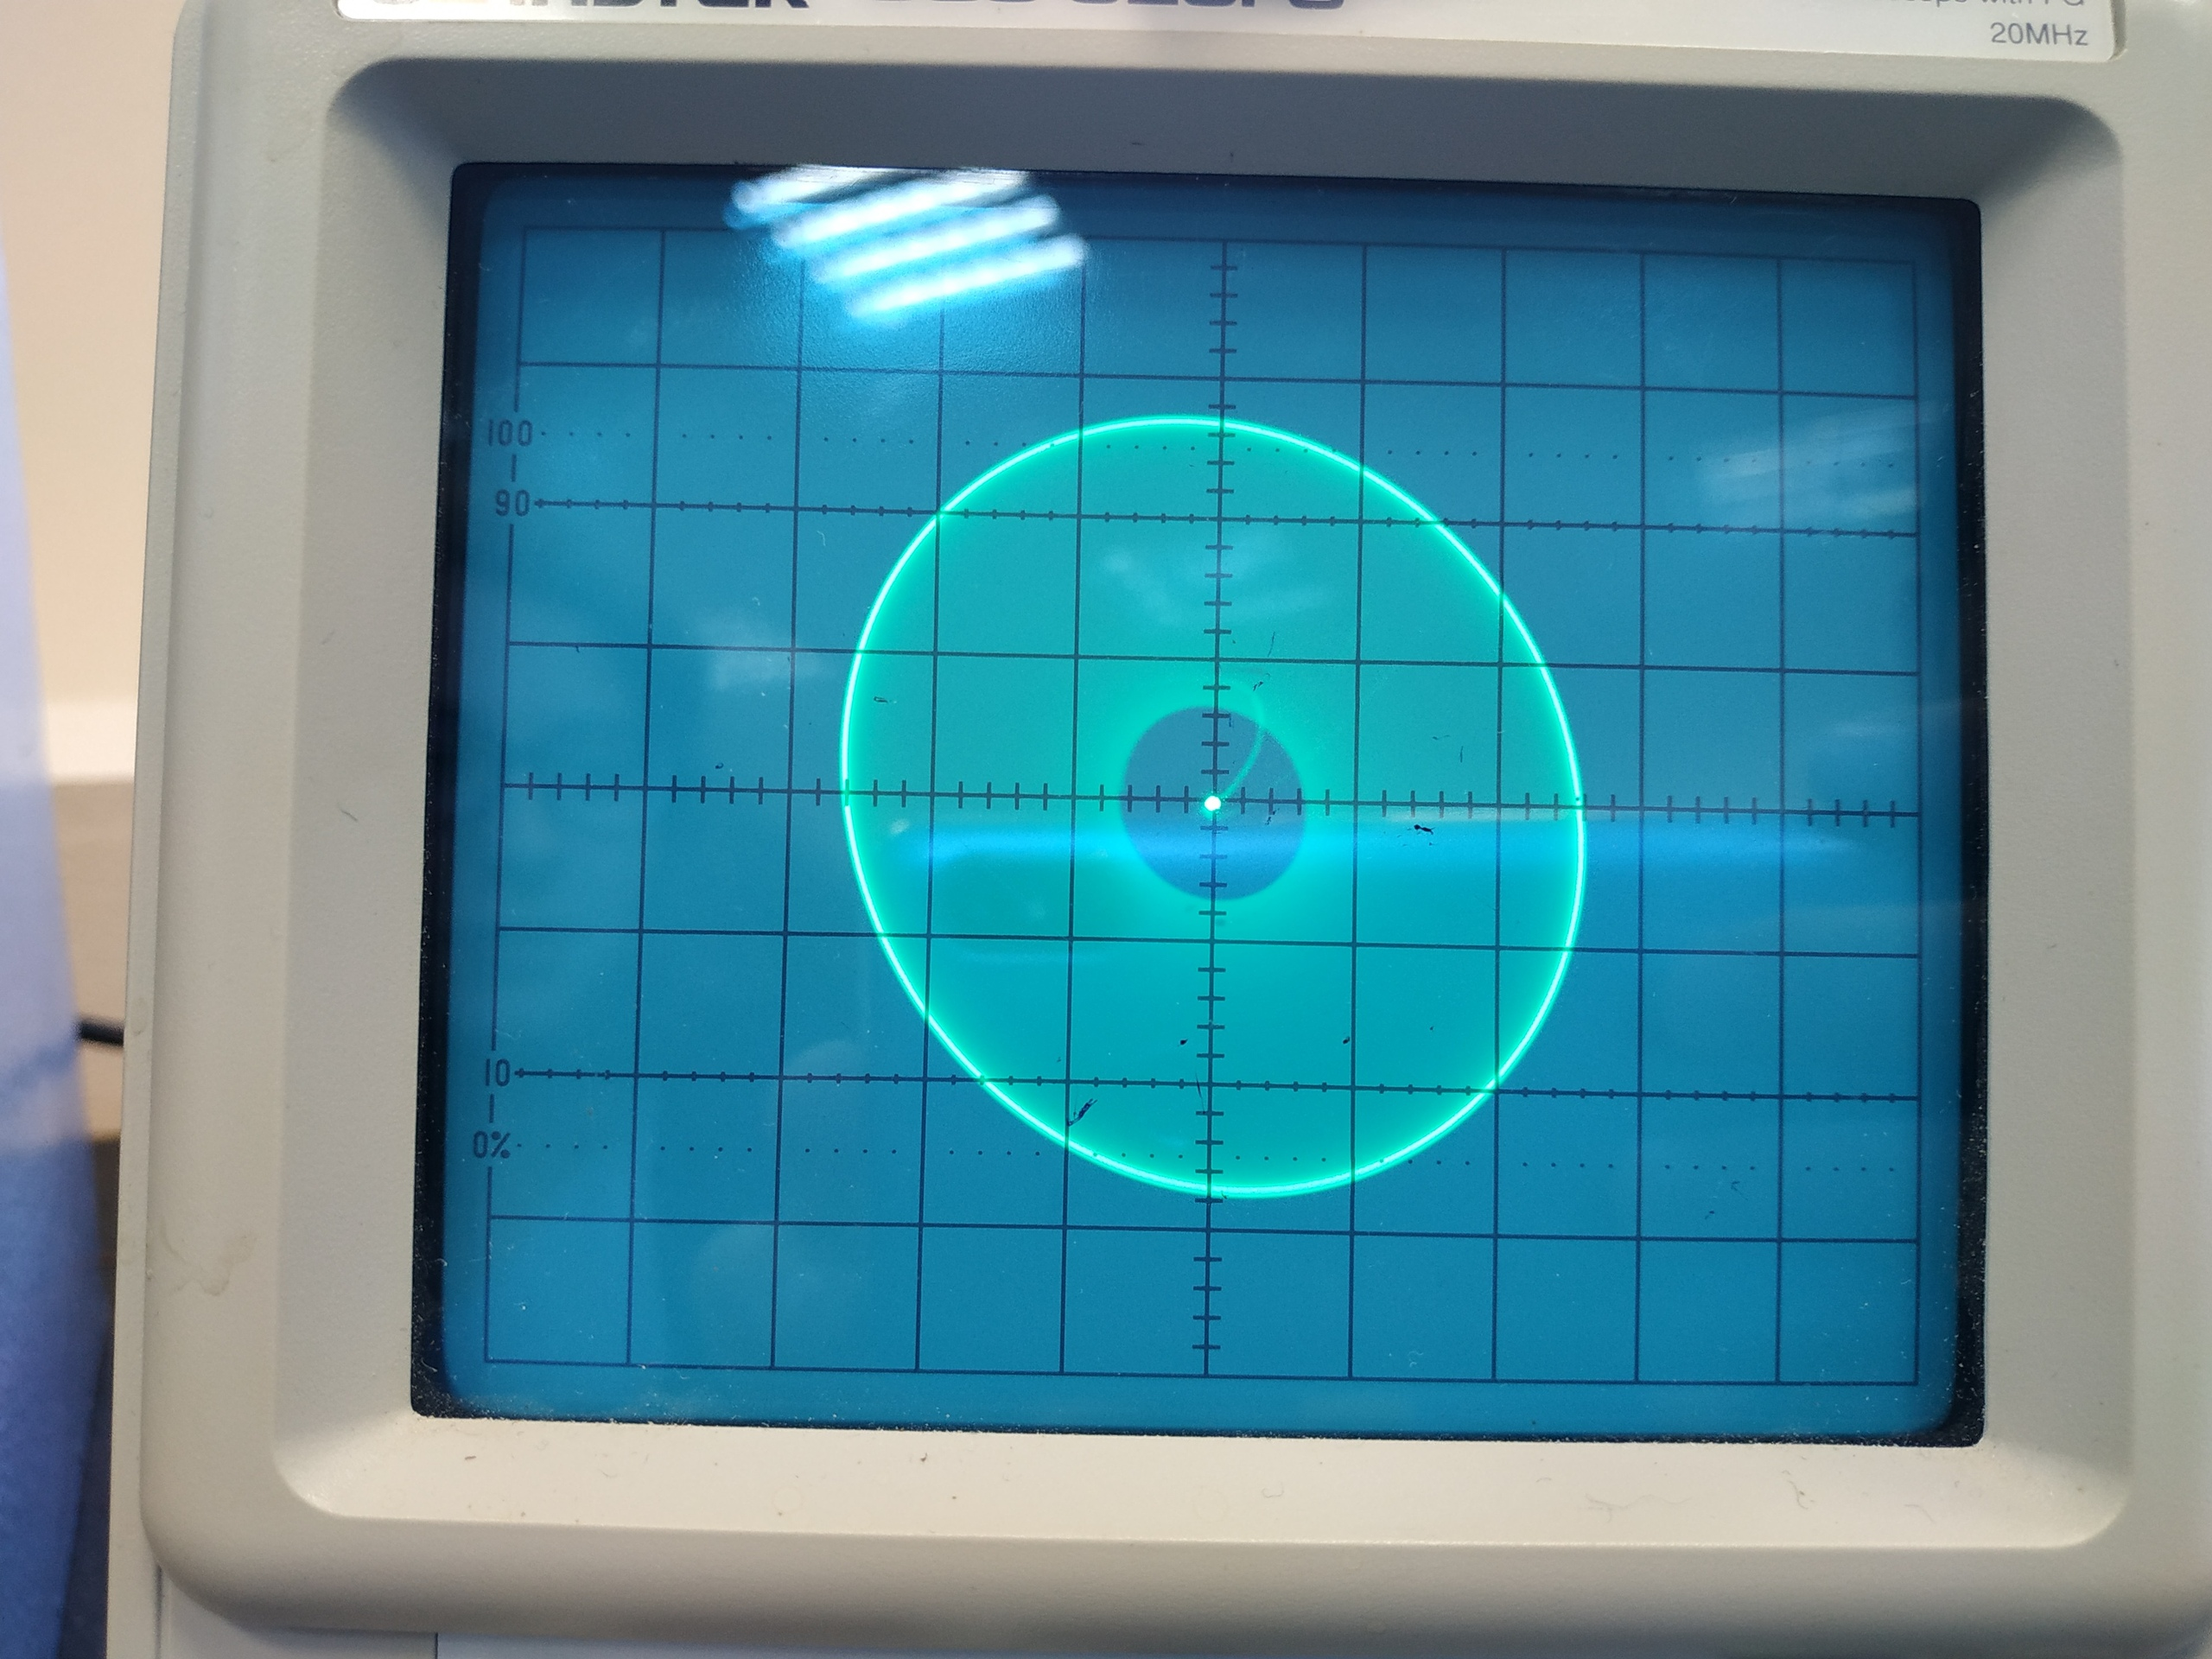
\includegraphics[height=150pt]{img/20.jpg} 
            \vspace{0pt}
            \label{fig:11}
            \captionof{subfigure}{} 
        \end{minipage}
        \begin{minipage}{0.49\linewidth}
            \centering
            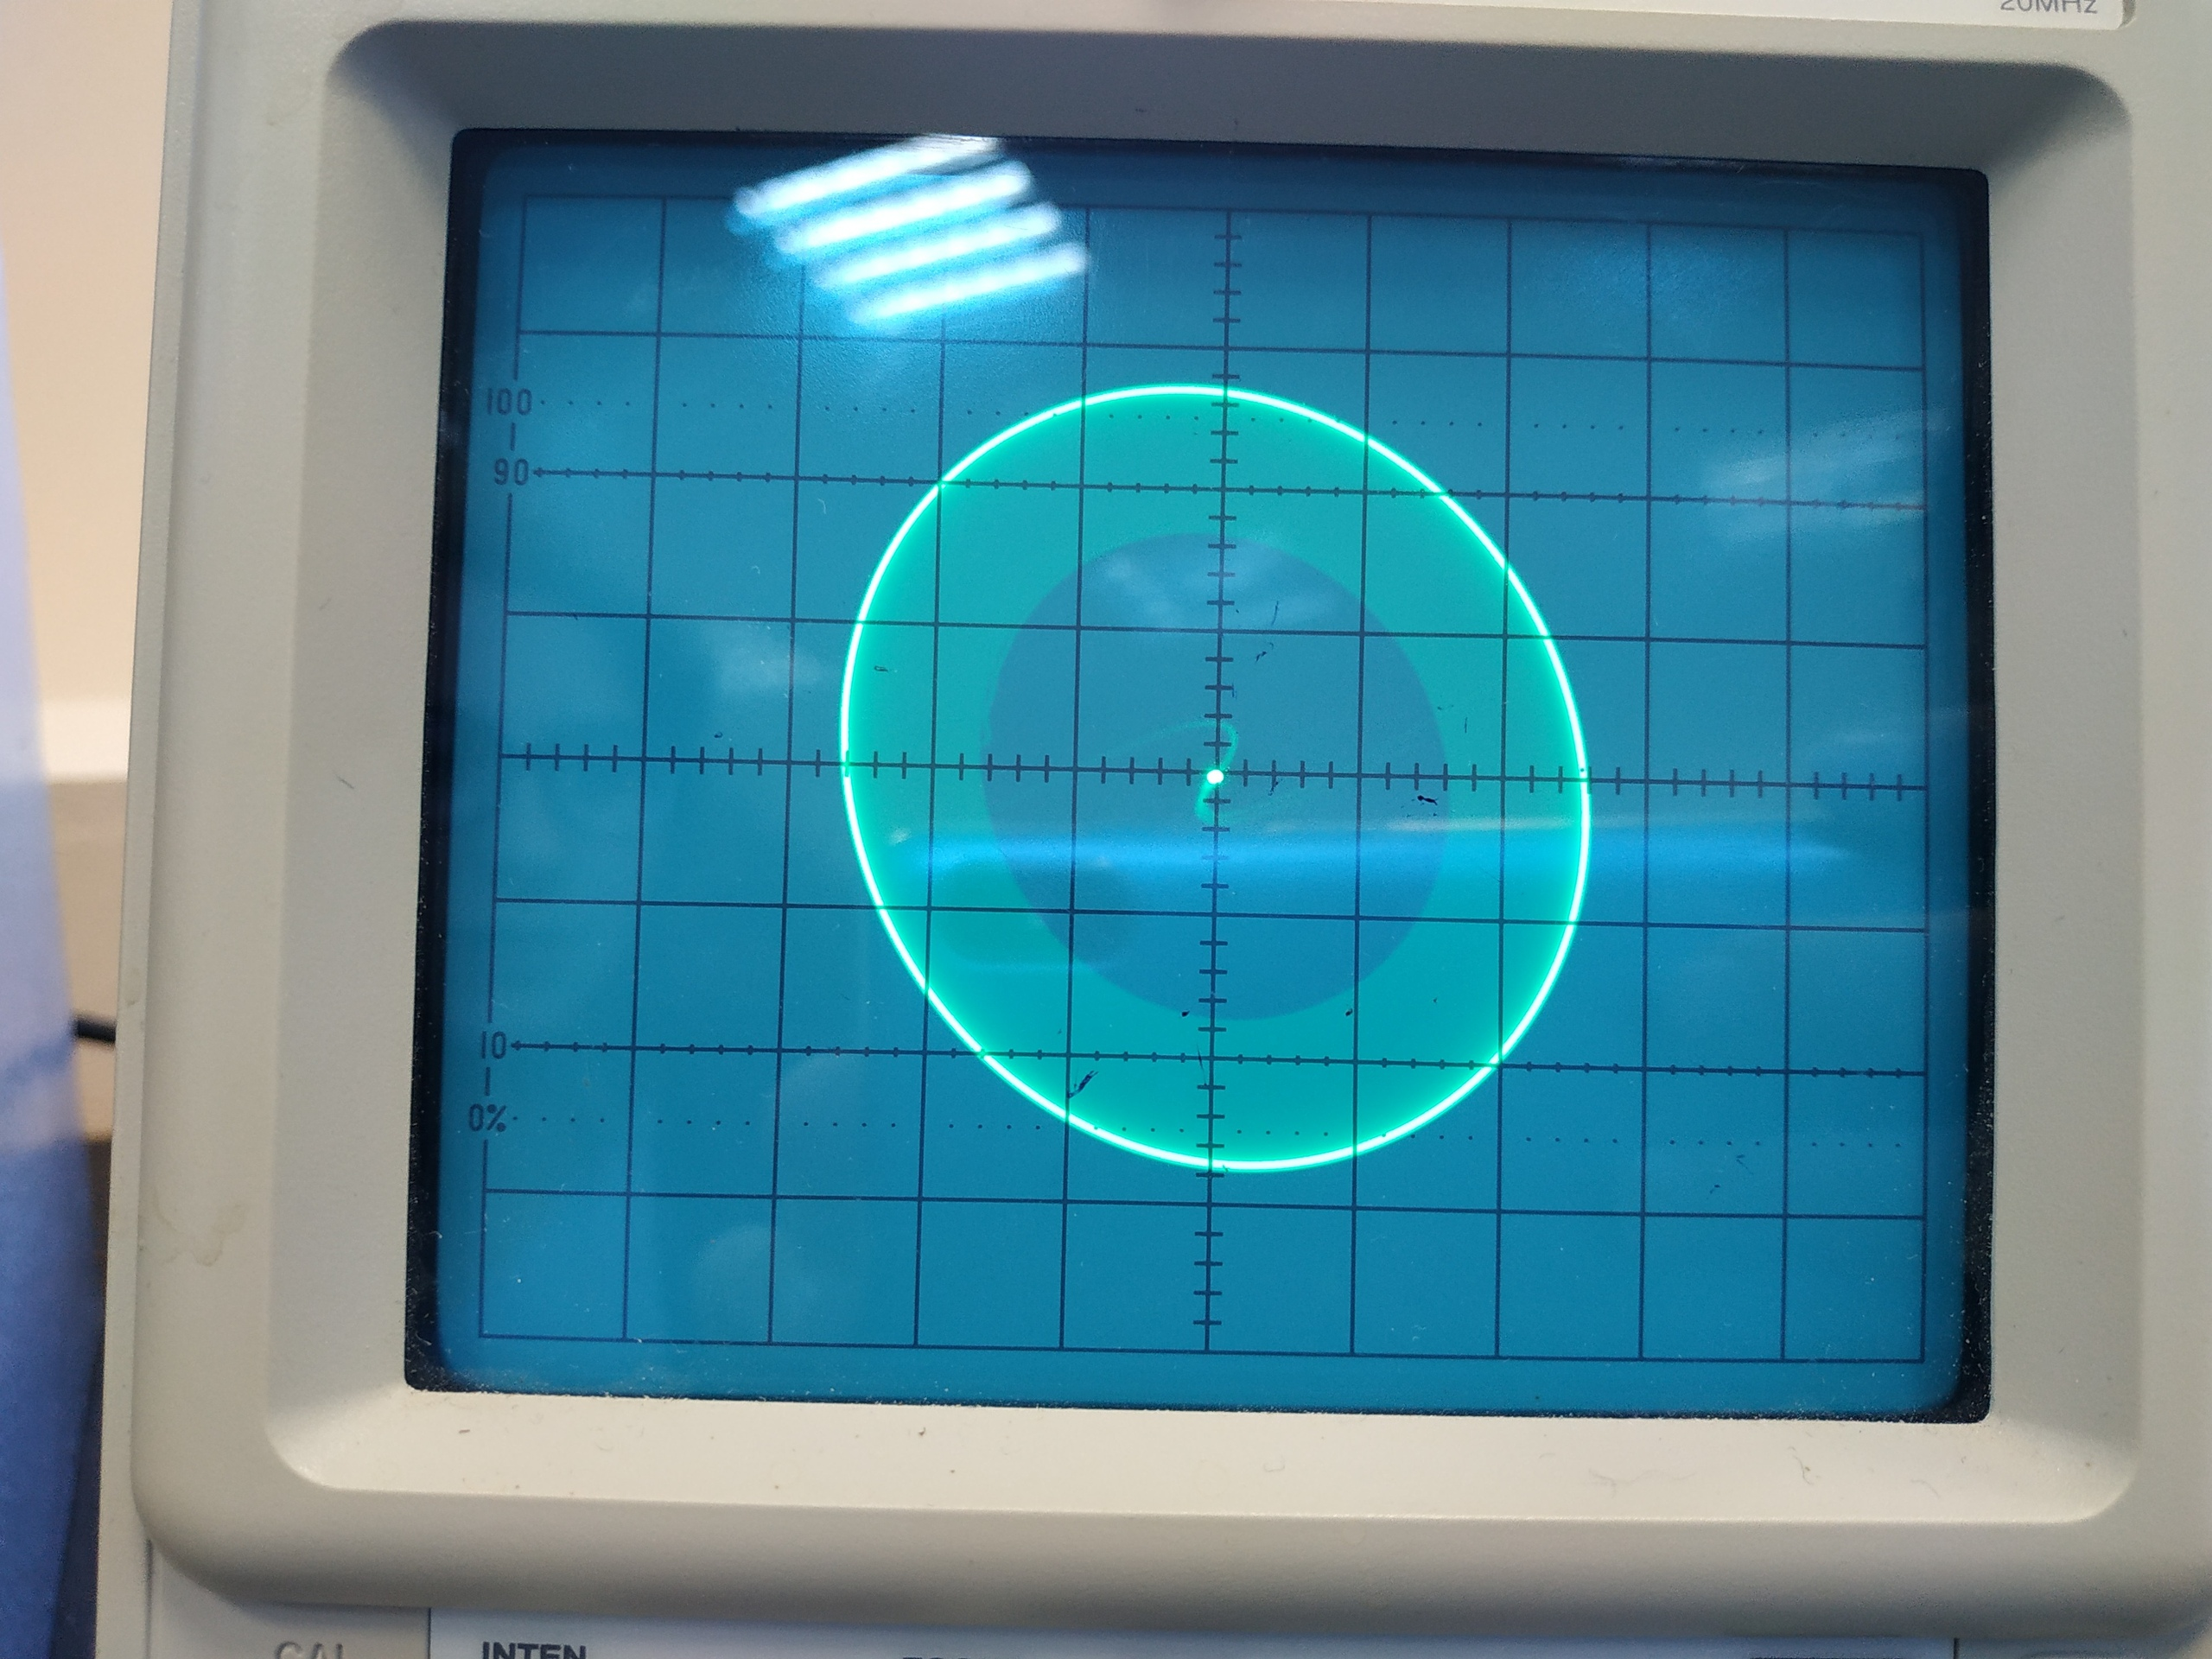
\includegraphics[height=150pt]{img/21.jpg} 
            \vspace{0pt}
            \label{fig:12}
            \captionof{subfigure}{} 
        \end{minipage}
    \caption{Фазовая траектория для $M'< M < M''$}
    \vspace{-40pt}
    \end{figure}
\end{center} 

\begin{center}
    \begin{figure}[H]
        \begin{minipage}{0.32\linewidth}
            \centering
            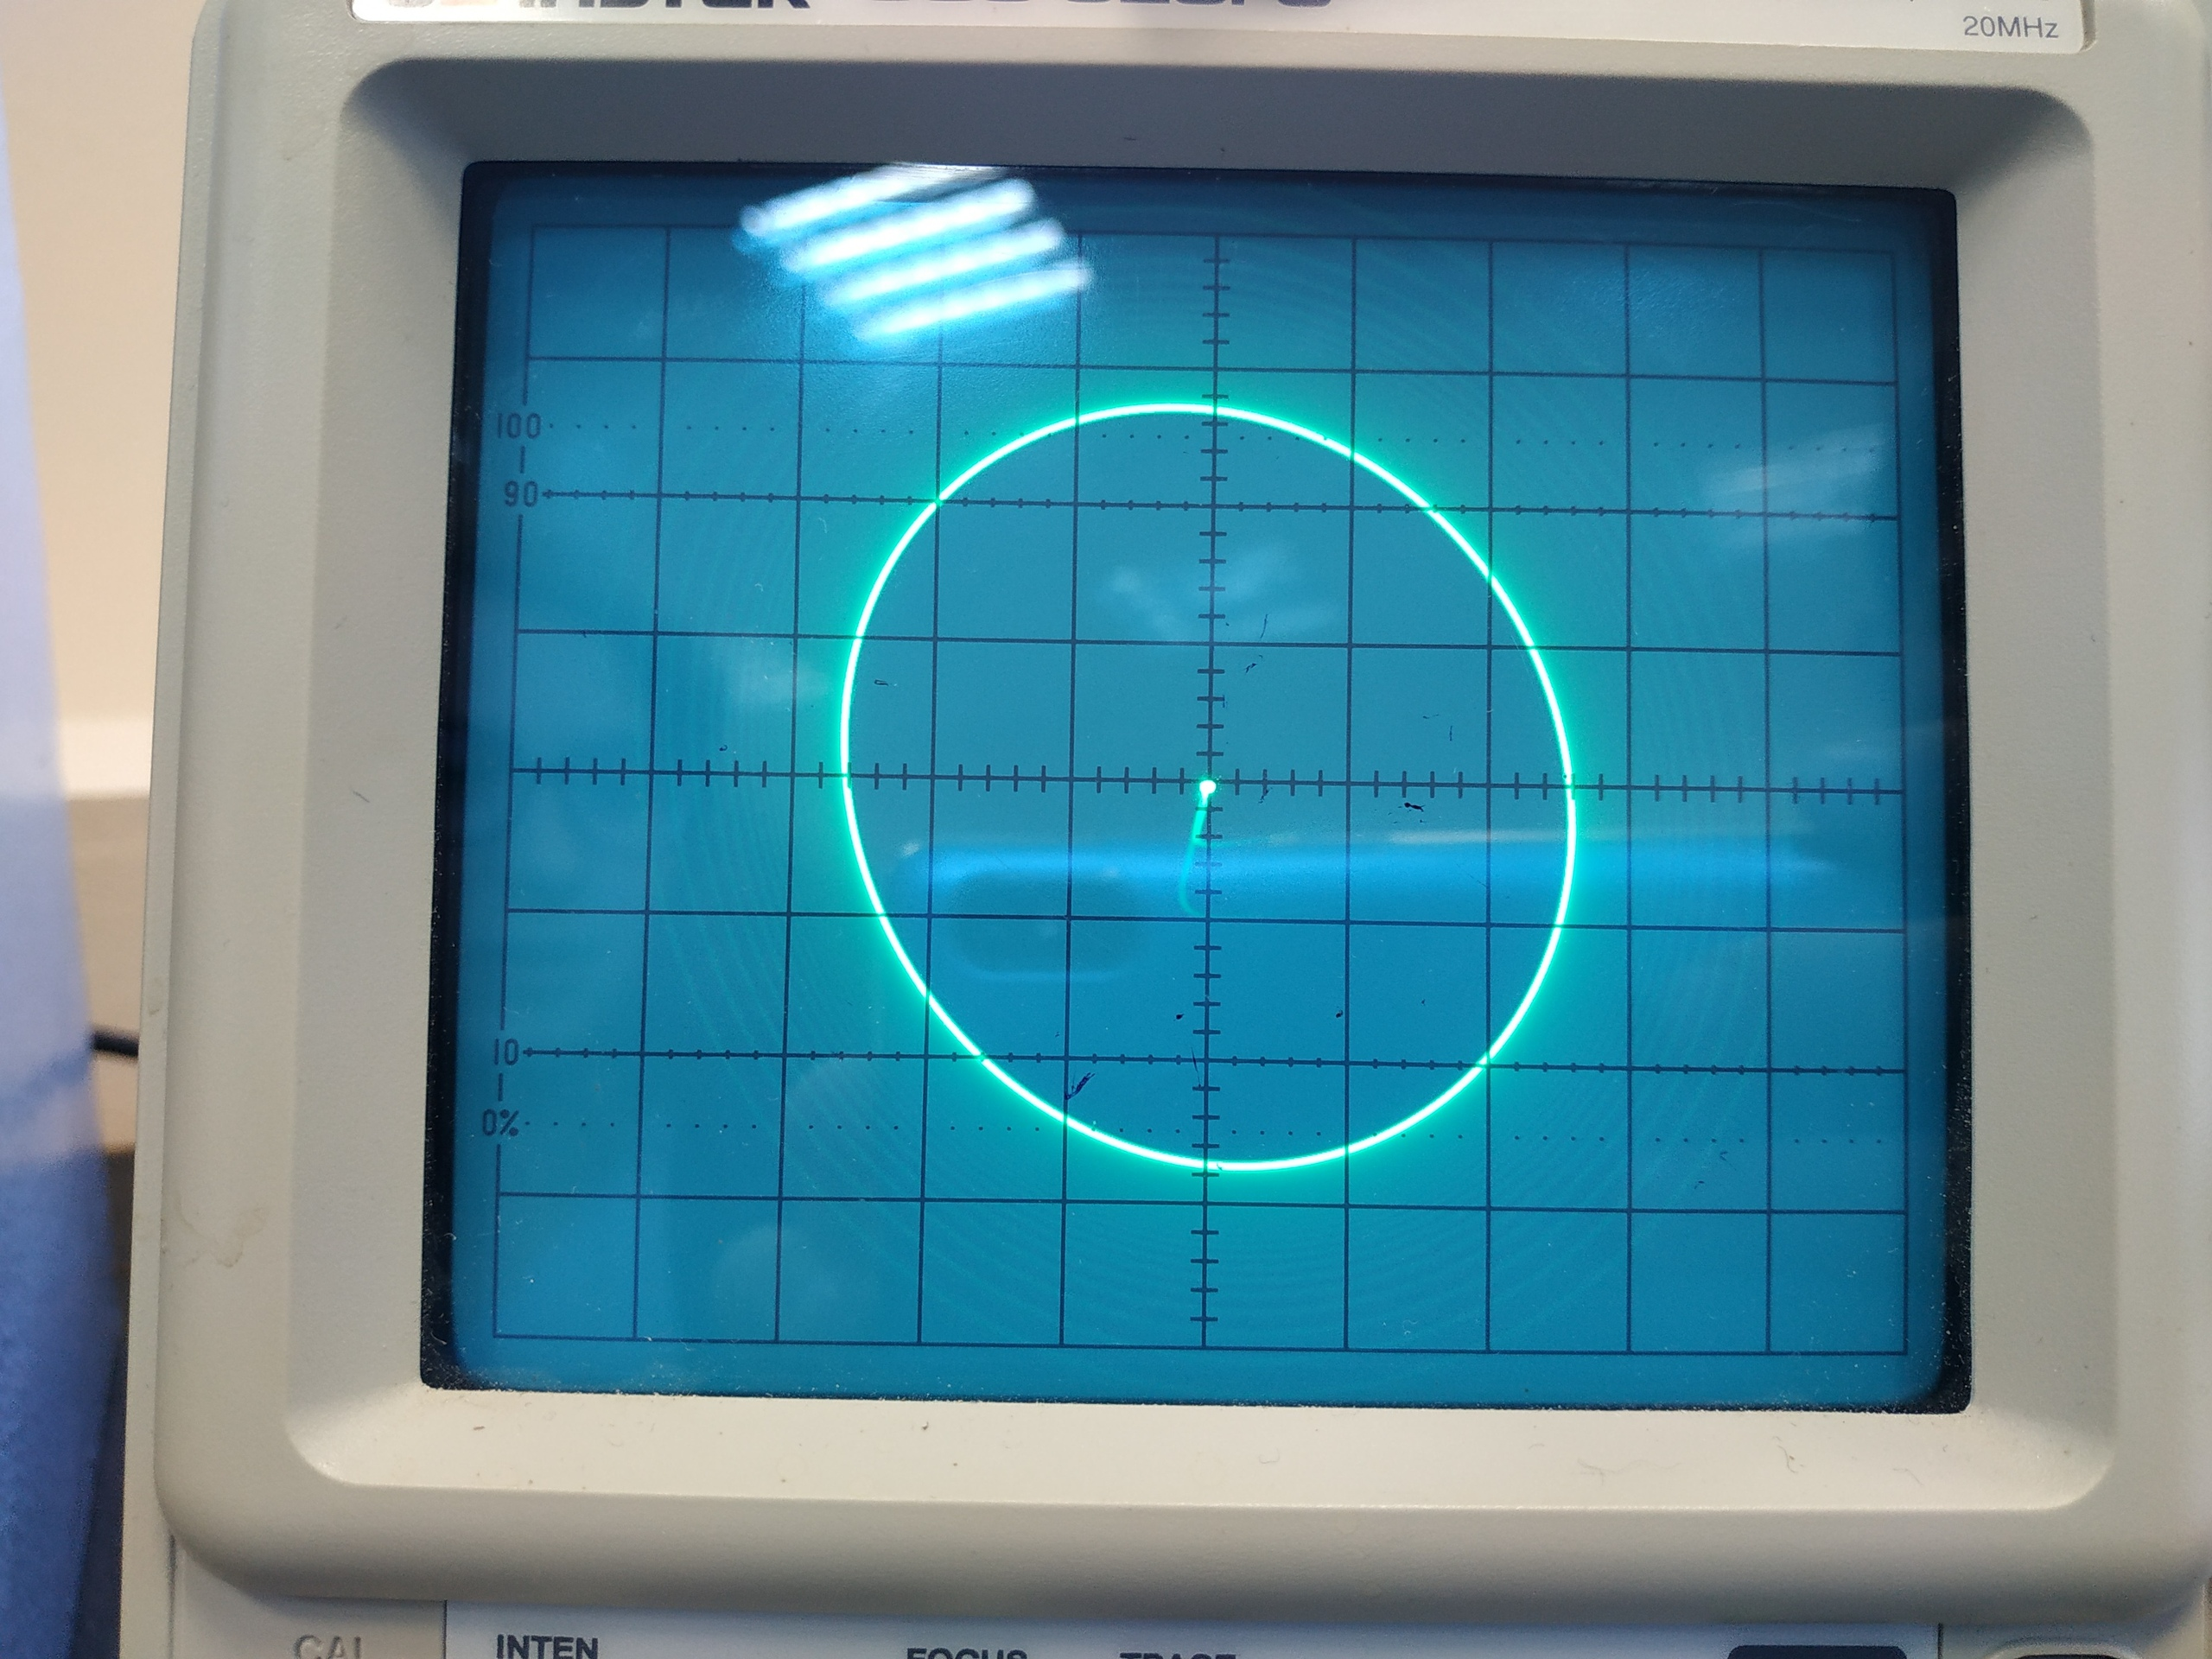
\includegraphics[height=100pt]{img/23.jpg} 
            \vspace{0pt}
            \label{fig:10}
            \captionof{subfigure}{} 
        \end{minipage}
        \begin{minipage}{0.32\linewidth}
            \centering
            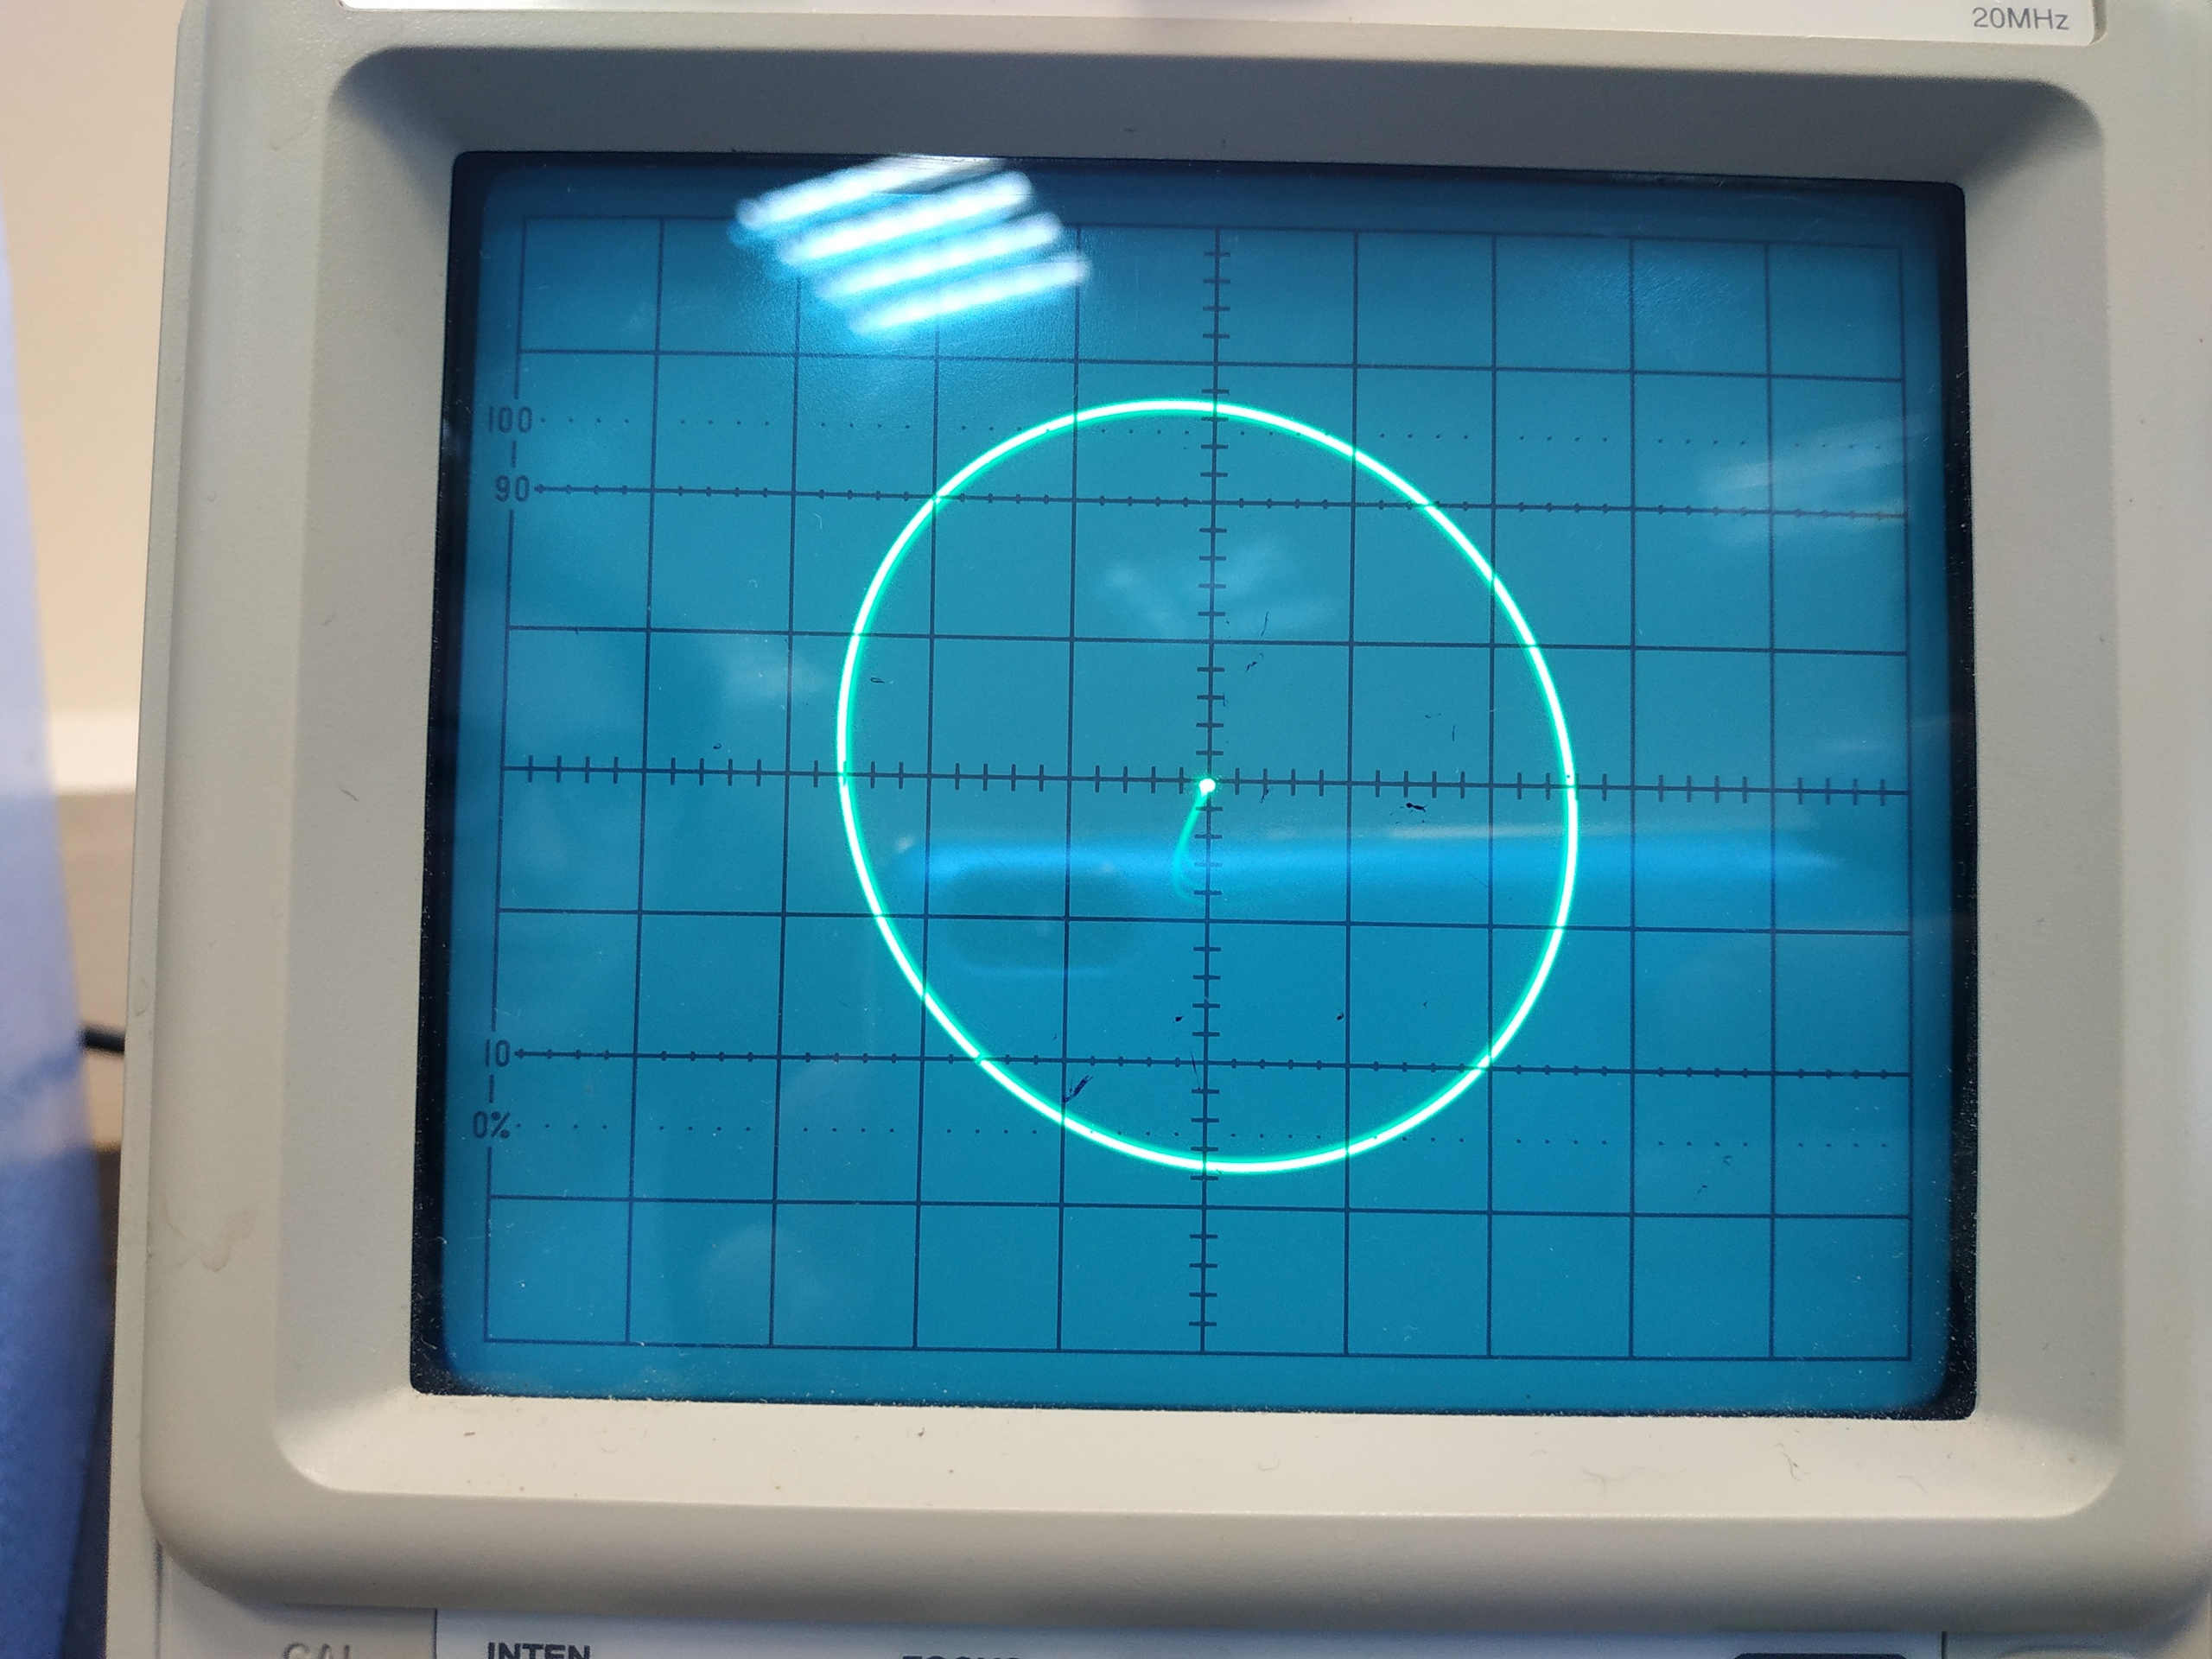
\includegraphics[height=100pt]{img/22.jpg} 
            \vspace{0pt}
            \label{fig:11}
            \captionof{subfigure}{} 
        \end{minipage}
        \begin{minipage}{0.32\linewidth}
            \centering
            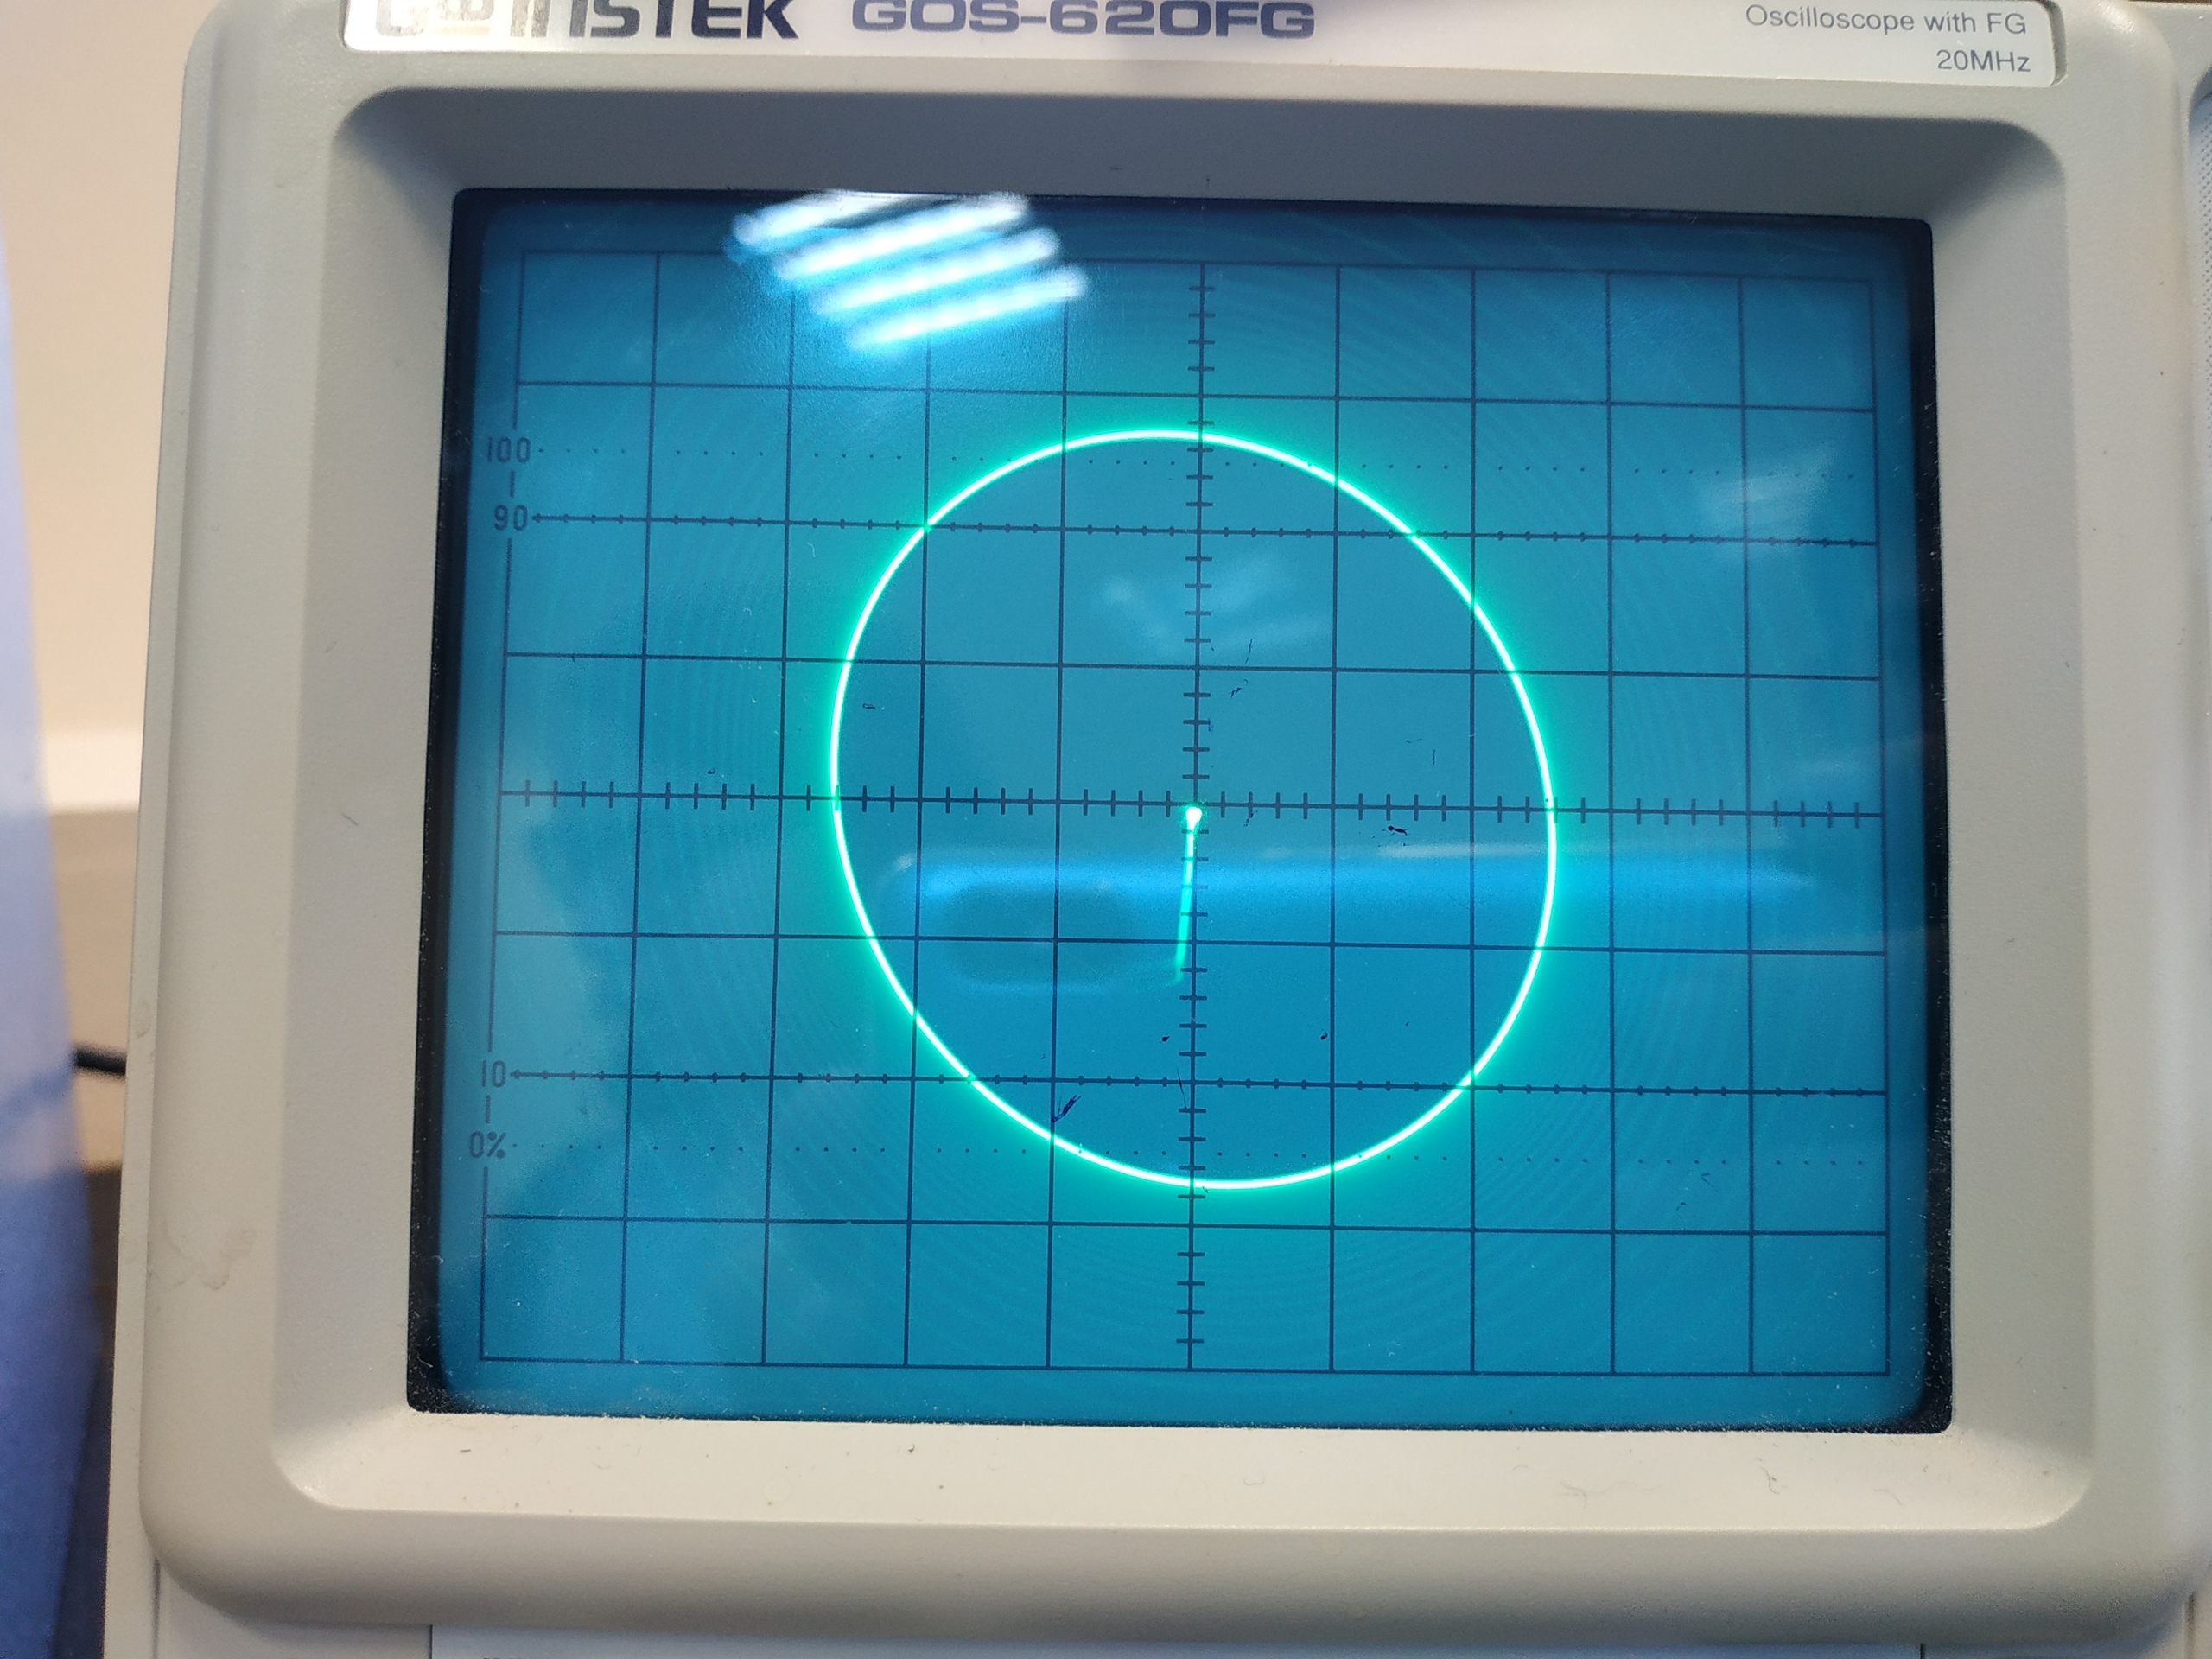
\includegraphics[height=100pt]{img/7.jpg} 
            \vspace{0pt}
            \label{fig:12}
            \captionof{subfigure}{} 
        \end{minipage}
    \caption{Фазовая траектория для $M''> M $}
    \vspace{-40pt}
    \end{figure}
\end{center} 

\subsection{Сложно-жесткий режим генератора}
Полученная бифуркационная диаграмма приведена на рис.23
\begin{center}
    \begin{figure}[H]
        \vspace{-10pt}
            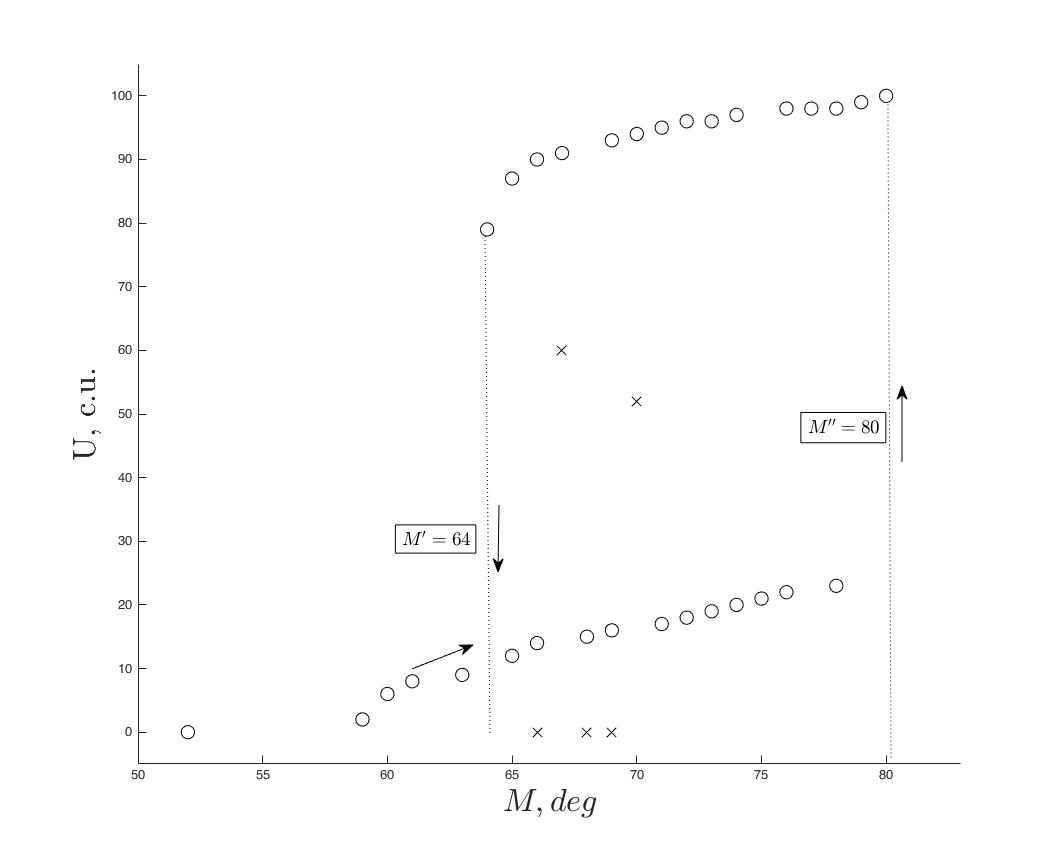
\includegraphics[width=\linewidth]{graph/g3} 
            \vspace{-10pt}
            \label{fig:10}
            \captionof{figure}{Бифуркационная диаграмма для сложно-жесткого режима генератора} 
            \vspace{-40pt}
    \end{figure}
\end{center} 
$$M'= 64 \pm 1 y.e.$$ $$M''= 80 \pm 1 y.e.$$ 
% Фазовые траектории для сильно-жесткого режима приведены на рис. 24 - рис. 26.
% \begin{center}
%     \begin{figure}[H]
%         \begin{minipage}{0.32\linewidth}
%             \centering
%             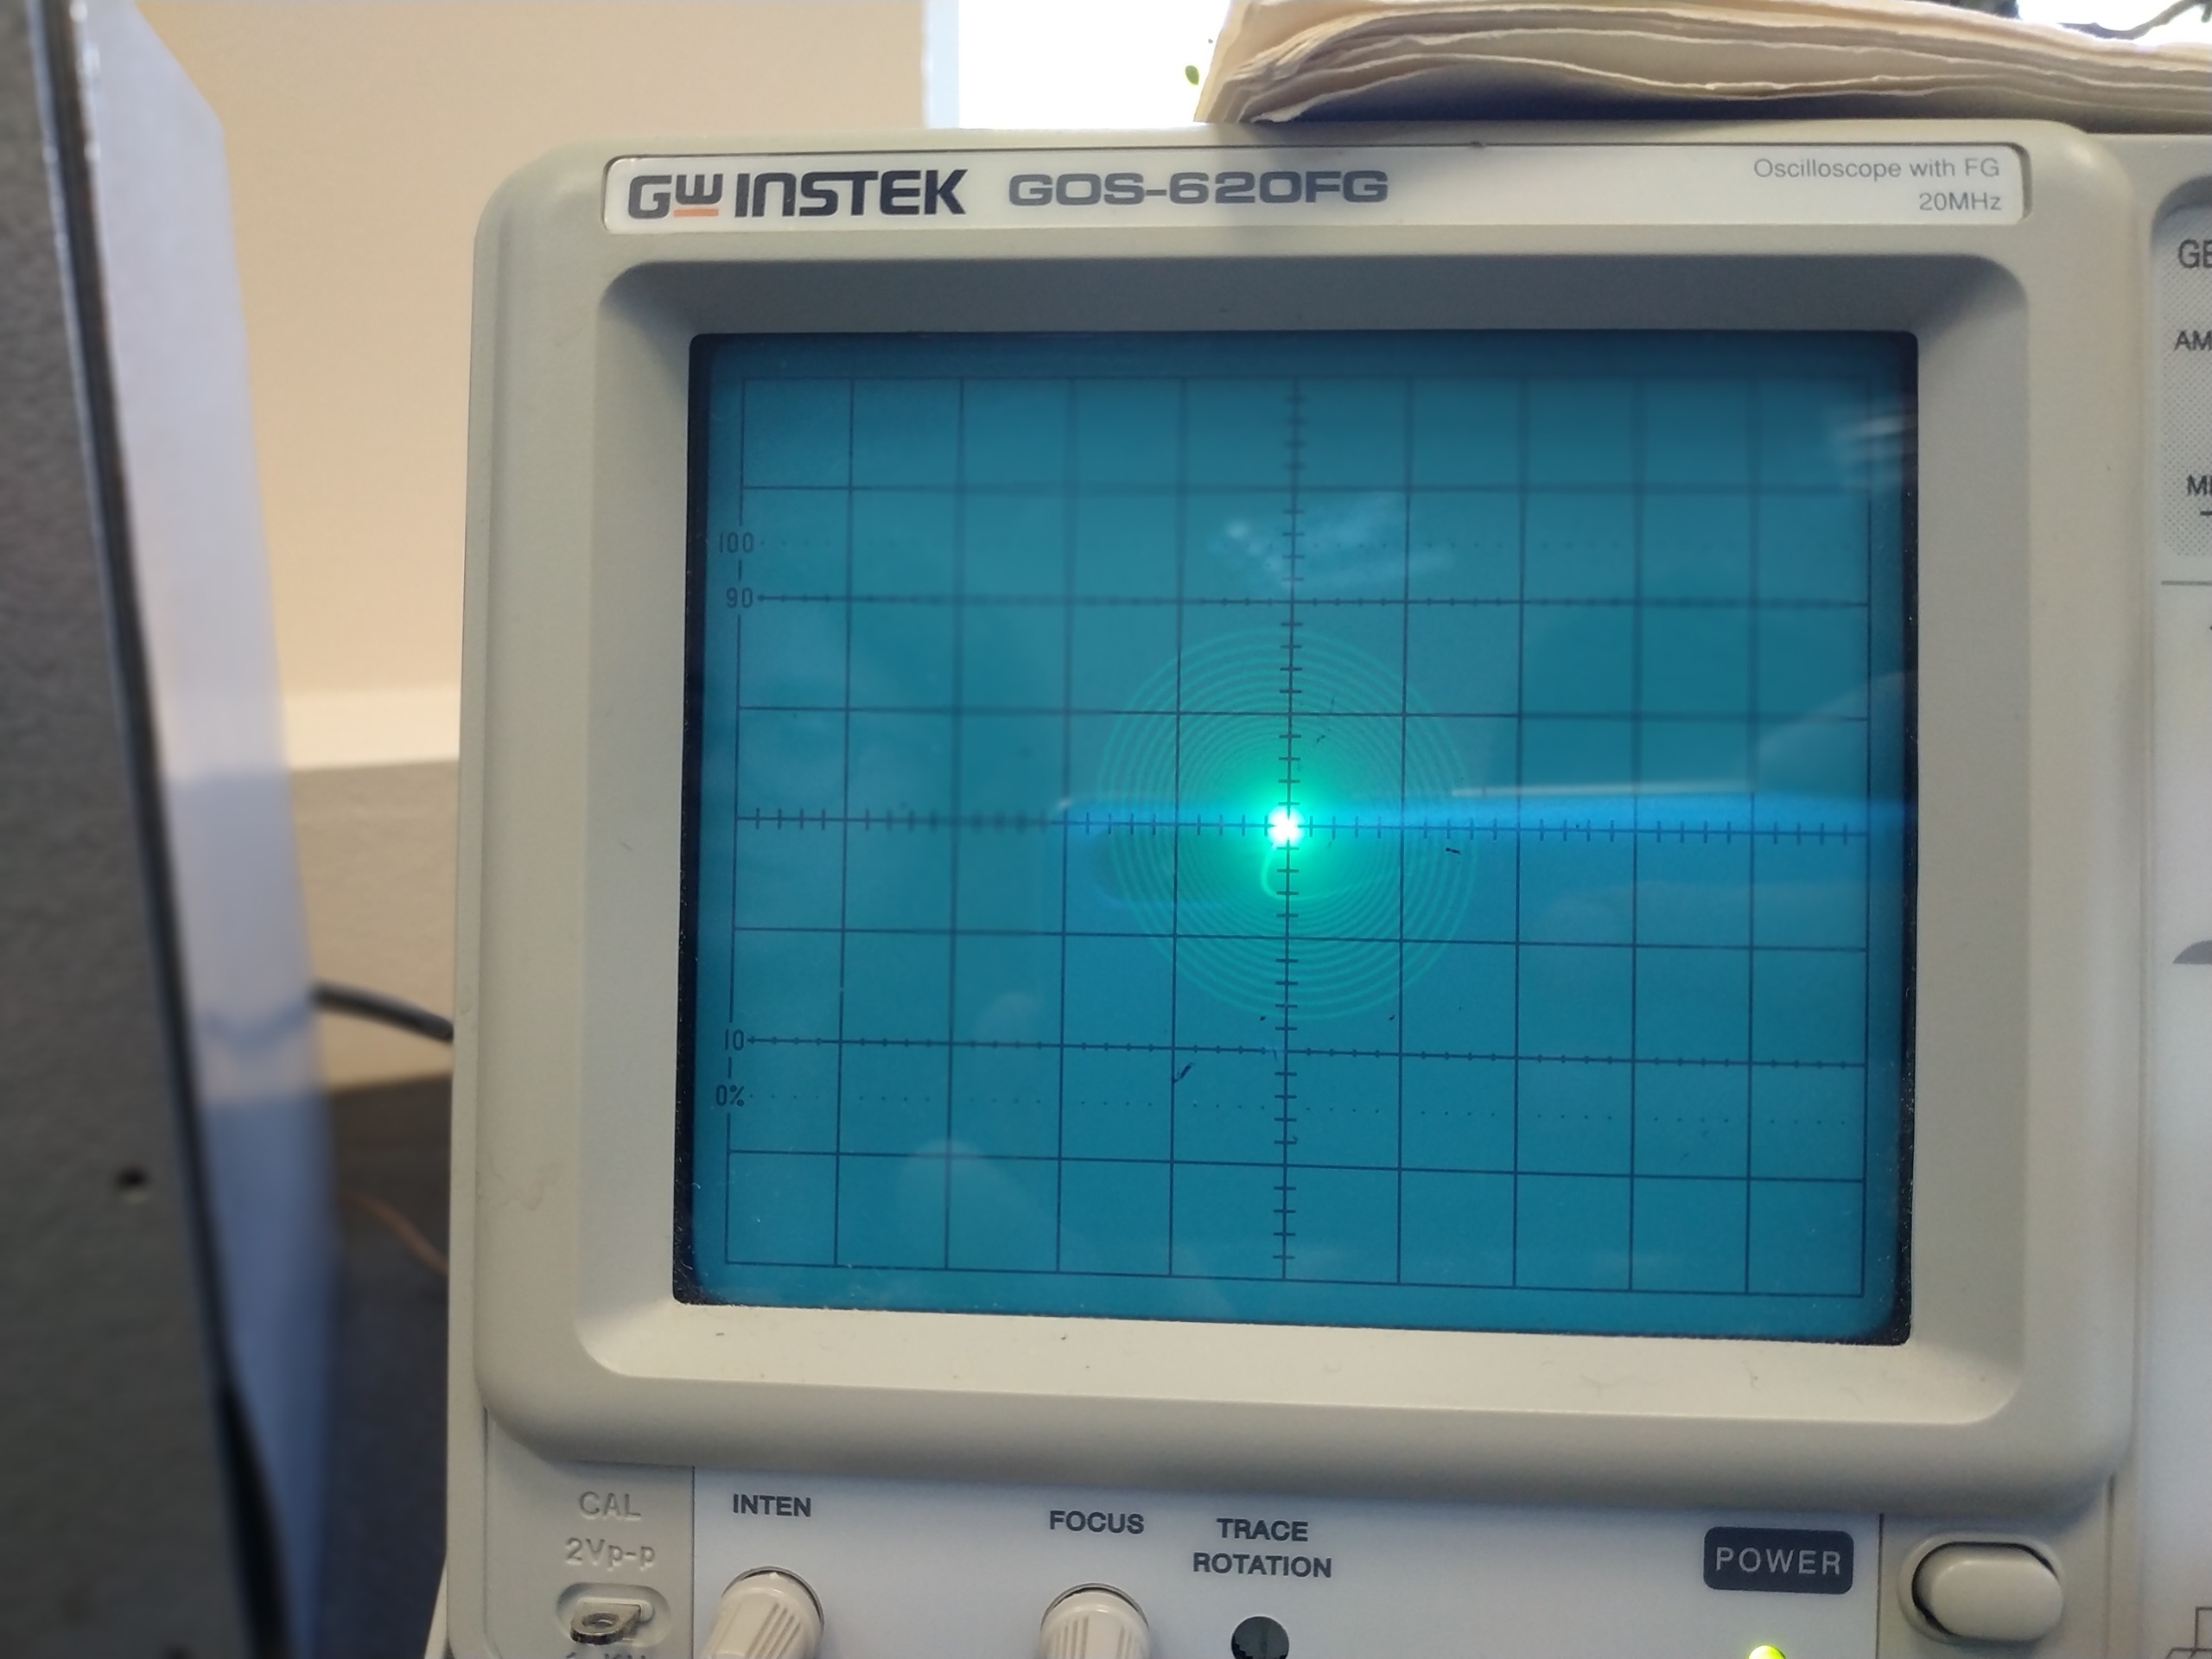
\includegraphics[height=100pt]{img/10.jpg} 
%             \vspace{0pt}
%             \label{fig:10}
%             \captionof{subfigure}{} 
%         \end{minipage}
%         \begin{minipage}{0.32\linewidth}
%             \centering
%             \includegraphics[height=100pt]{img/26.jpg} 
%             \vspace{0pt}
%             \label{fig:11}
%             \captionof{subfigure}{} 
%         \end{minipage}
%         \begin{minipage}{0.32\linewidth}
%             \centering
%             \includegraphics[height=100pt]{img/25.jpg} 
%             \vspace{0pt}
%             \label{fig:12}
%             \captionof{subfigure}{} 
%         \end{minipage}
%     \caption{Фазовая траектория для $M < M'$}
%     \vspace{-40pt}
%     \end{figure}
% \end{center} 

% \begin{center}
%     \begin{figure}[H]
%         \begin{minipage}{0.32\linewidth}
%             \centering
%             \includegraphics[height=100pt]{img/24.jpg} 
%             \vspace{0pt}
%             \label{fig:10}
%             \captionof{subfigure}{} 
%         \end{minipage}
%         \begin{minipage}{0.32\linewidth}
%             \centering
%             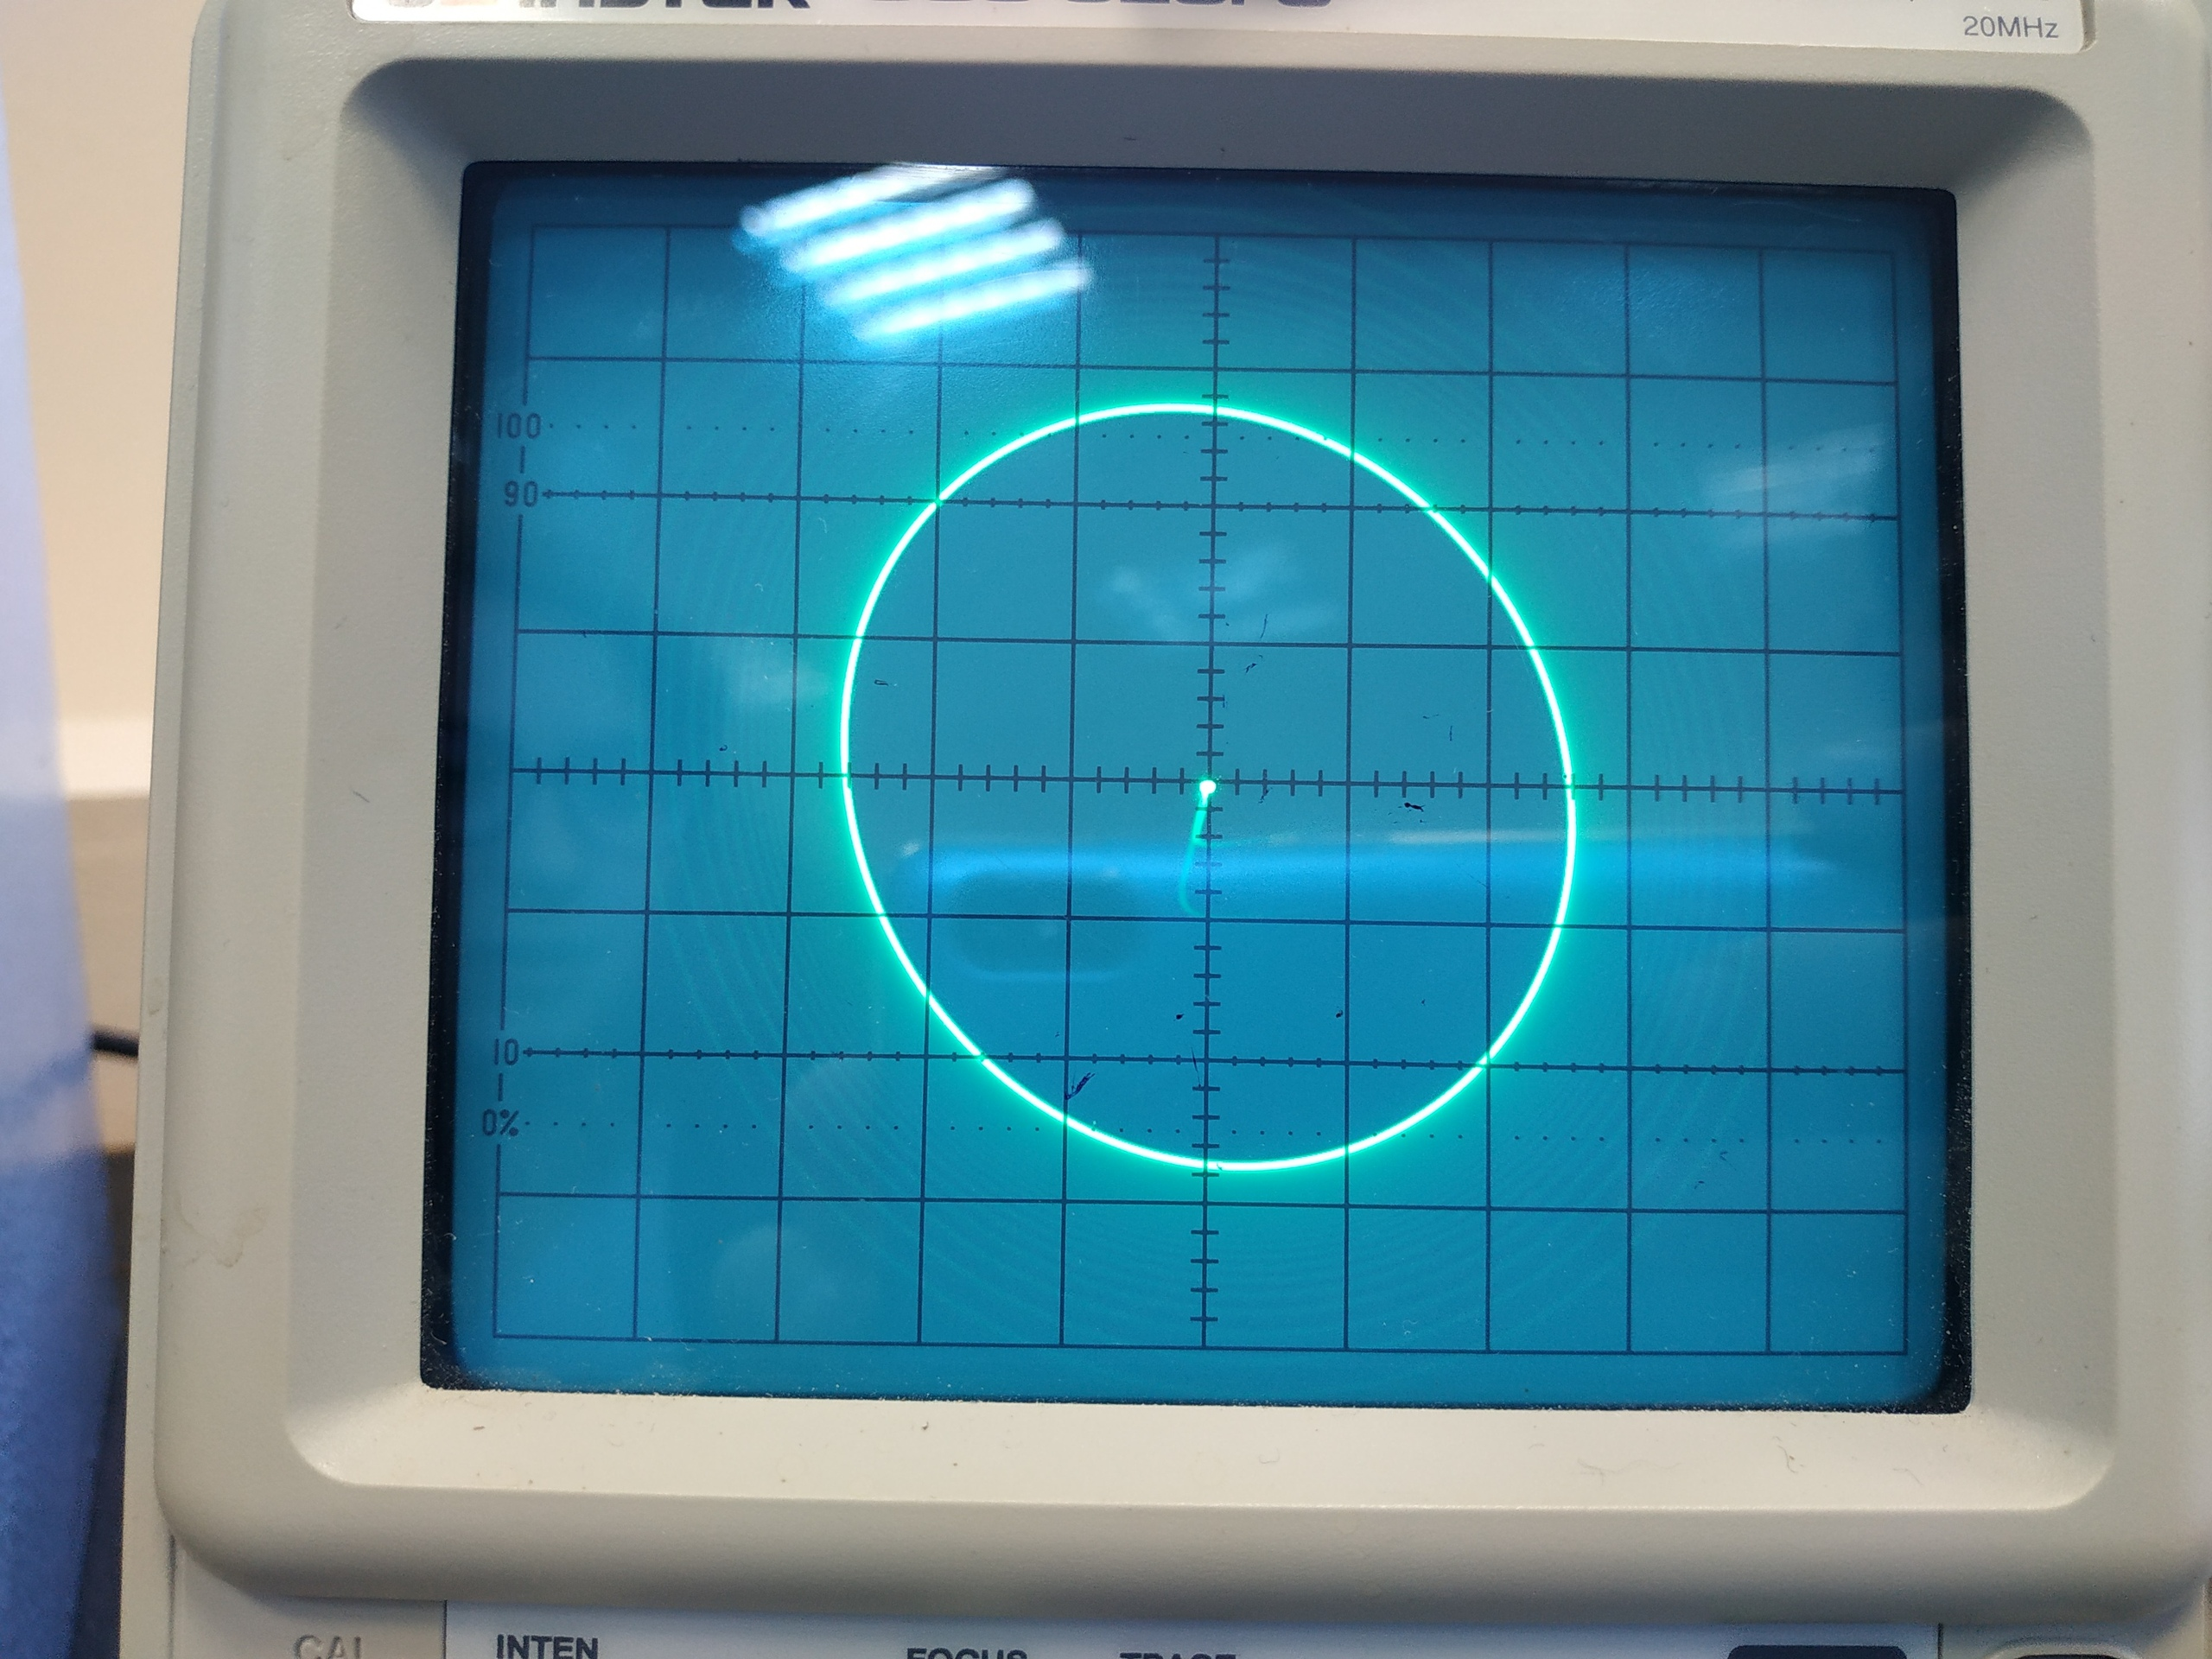
\includegraphics[height=100pt]{img/23.jpg} 
%             \vspace{0pt}
%             \label{fig:11}
%             \captionof{subfigure}{} 
%         \end{minipage}
%         \begin{minipage}{0.32\linewidth}
%             \centering
%             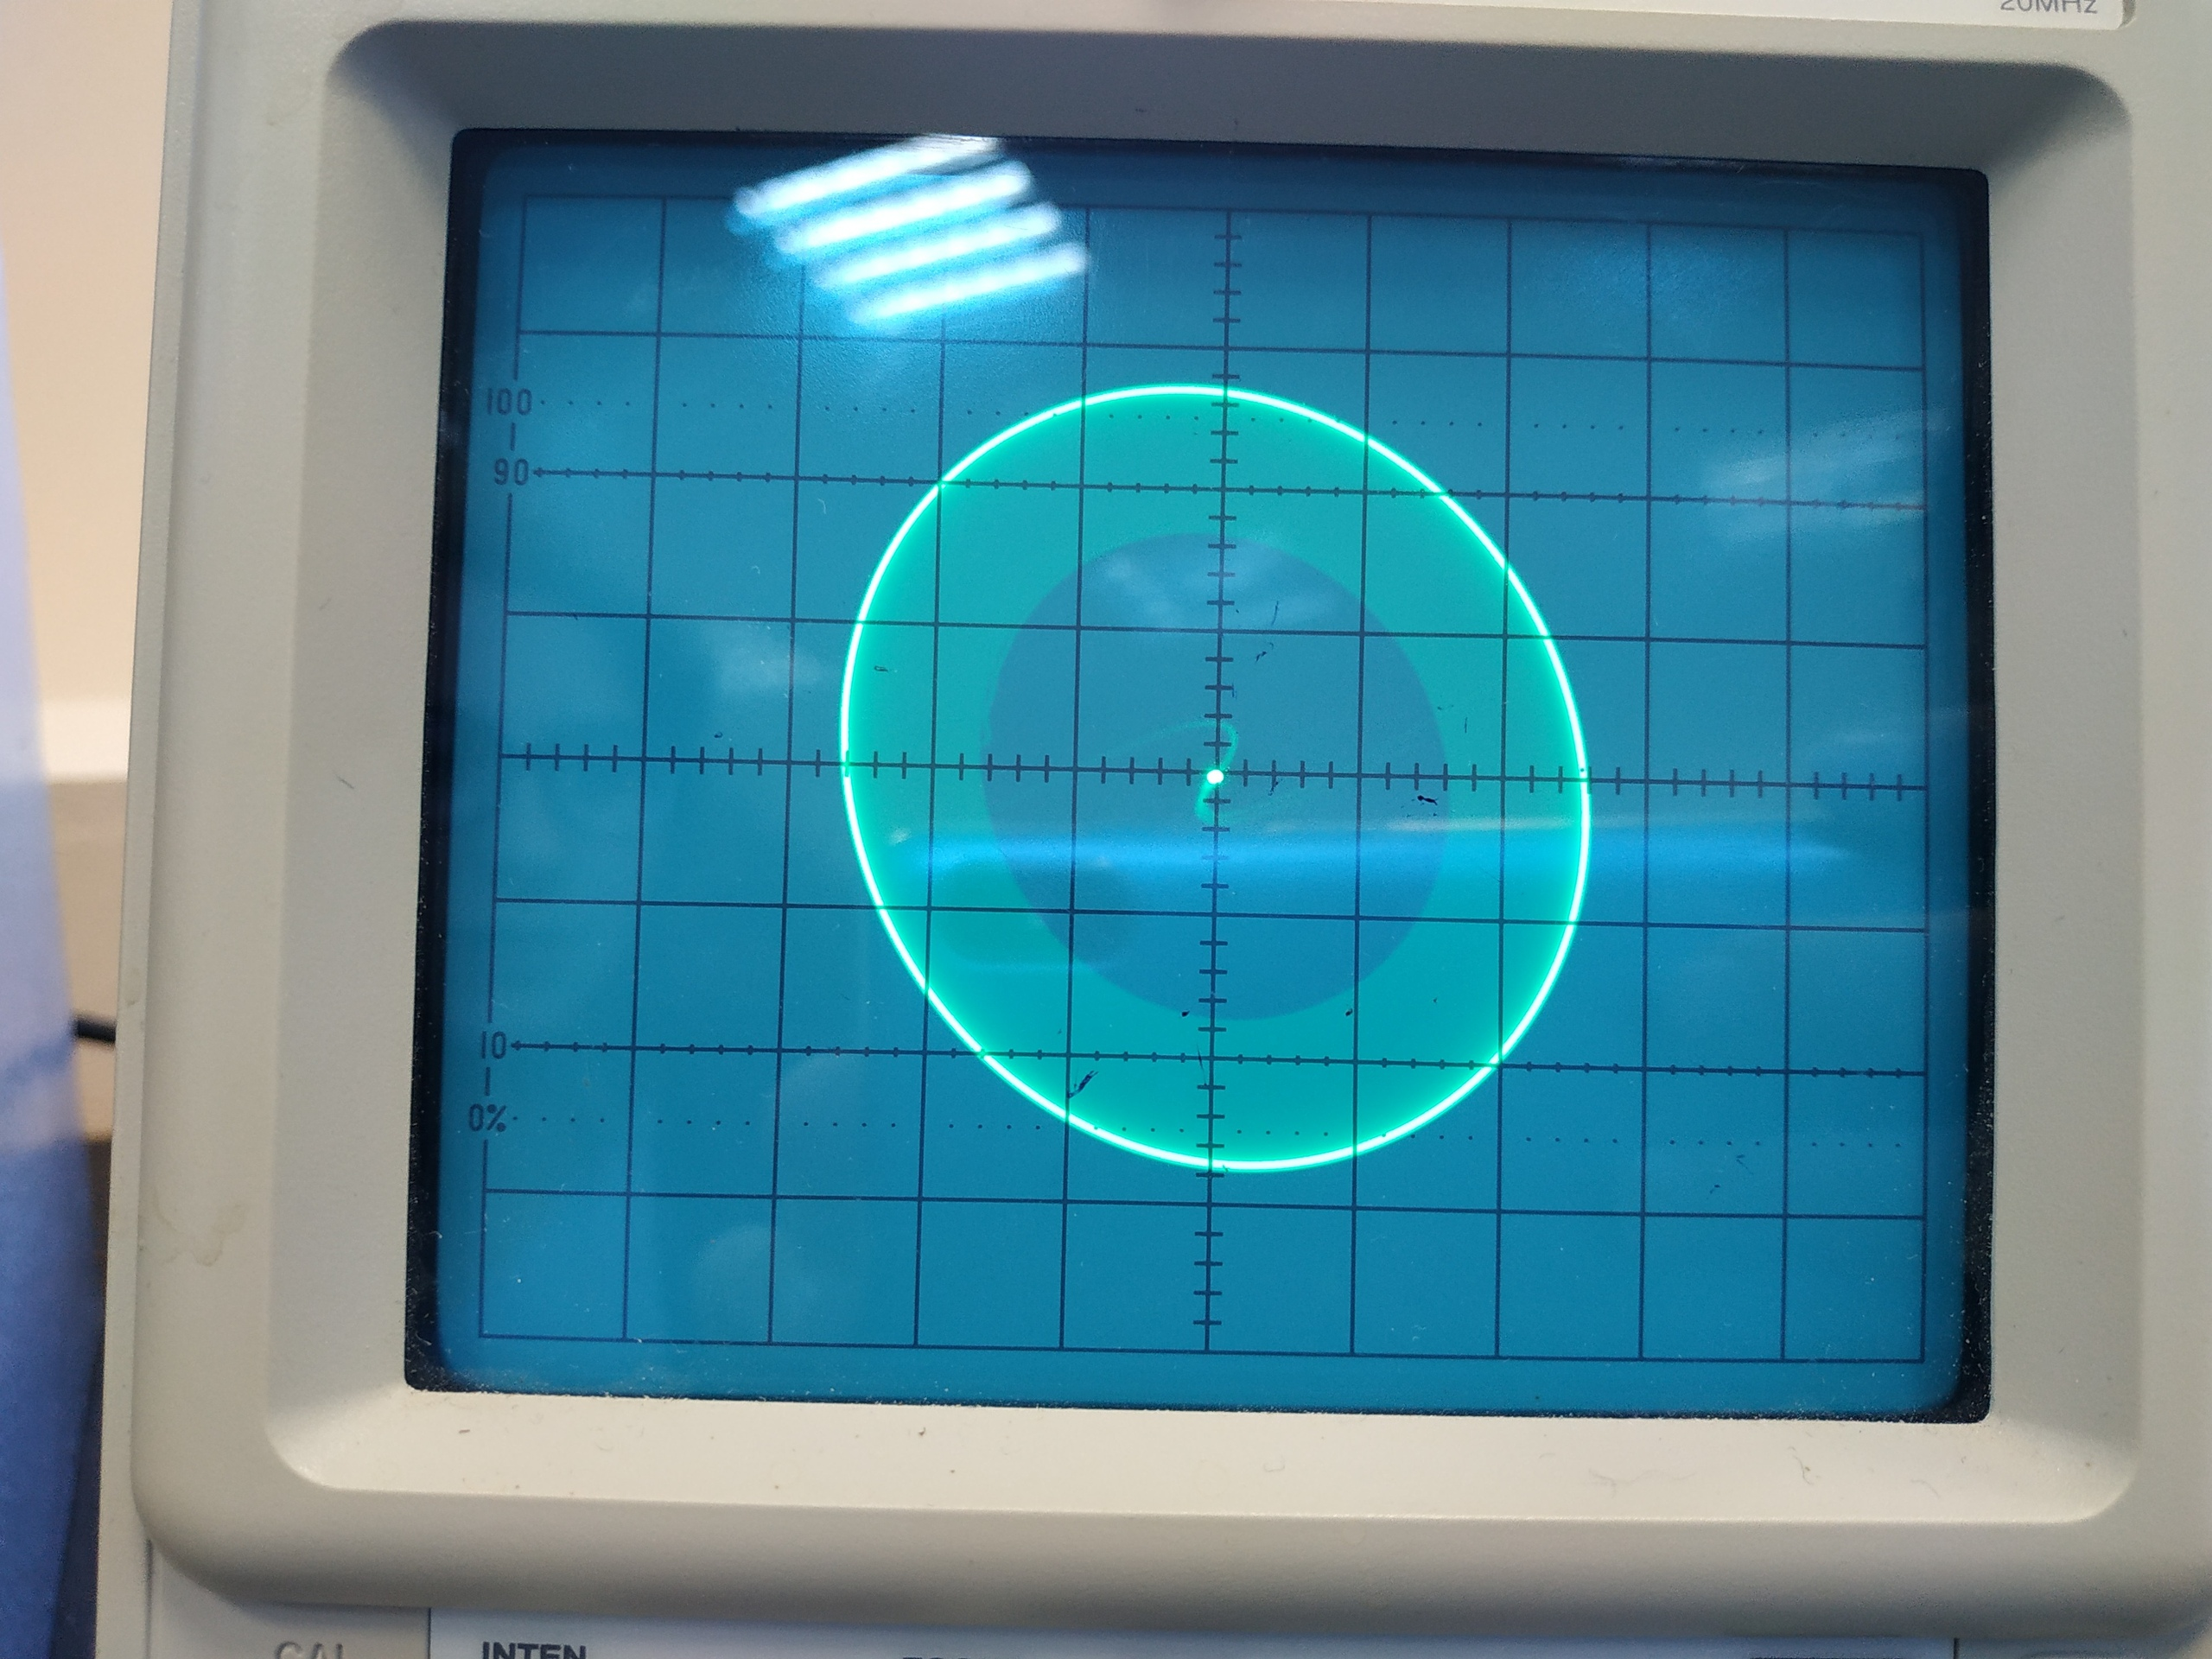
\includegraphics[height=100pt]{img/21.jpg} 
%             \vspace{0pt}
%             \label{fig:12}
%             \captionof{subfigure}{} 
%         \end{minipage}
%     \caption{Фазовая траектория для $M'< M < M''$}
%     \vspace{-40pt}
%     \end{figure}
% \end{center} 

% \begin{center}
%     \begin{figure}[H]
%         \begin{minipage}{0.32\linewidth}
%             \centering
%             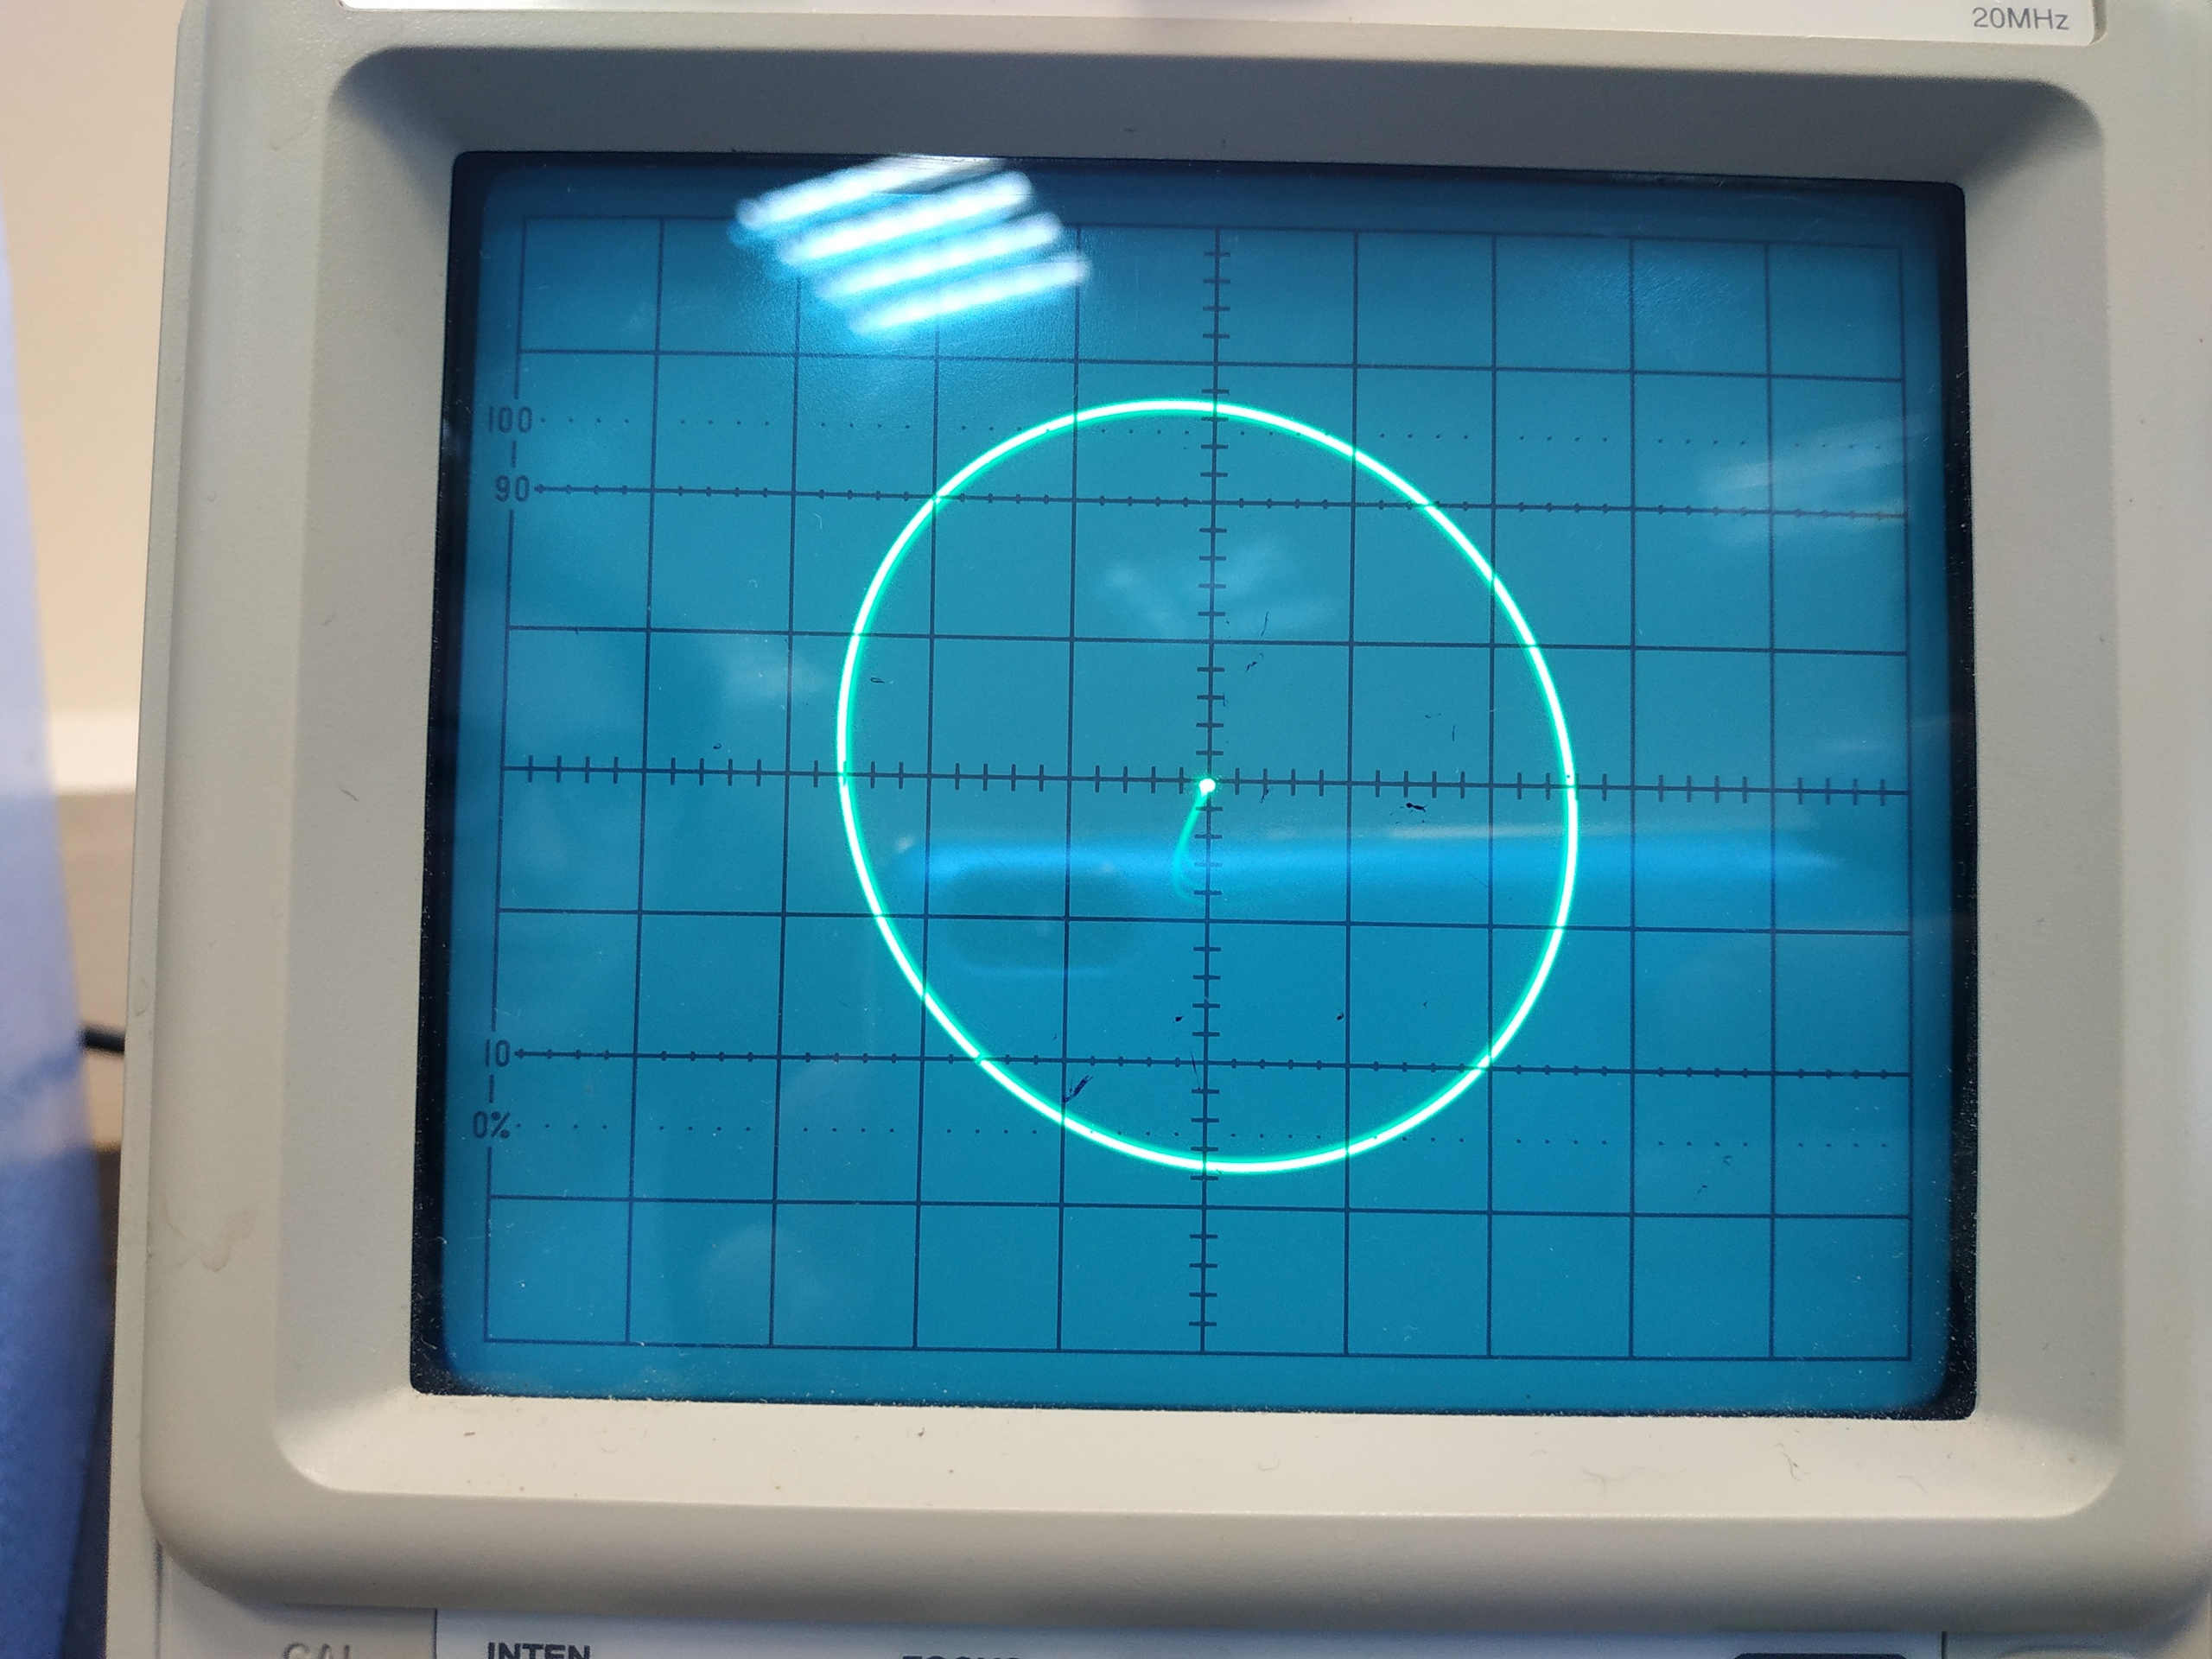
\includegraphics[height=100pt]{img/22.jpg} 
%             \vspace{0pt}
%             \label{fig:10}
%             \captionof{subfigure}{} 
%         \end{minipage}
%         \begin{minipage}{0.32\linewidth}
%             \centering
%             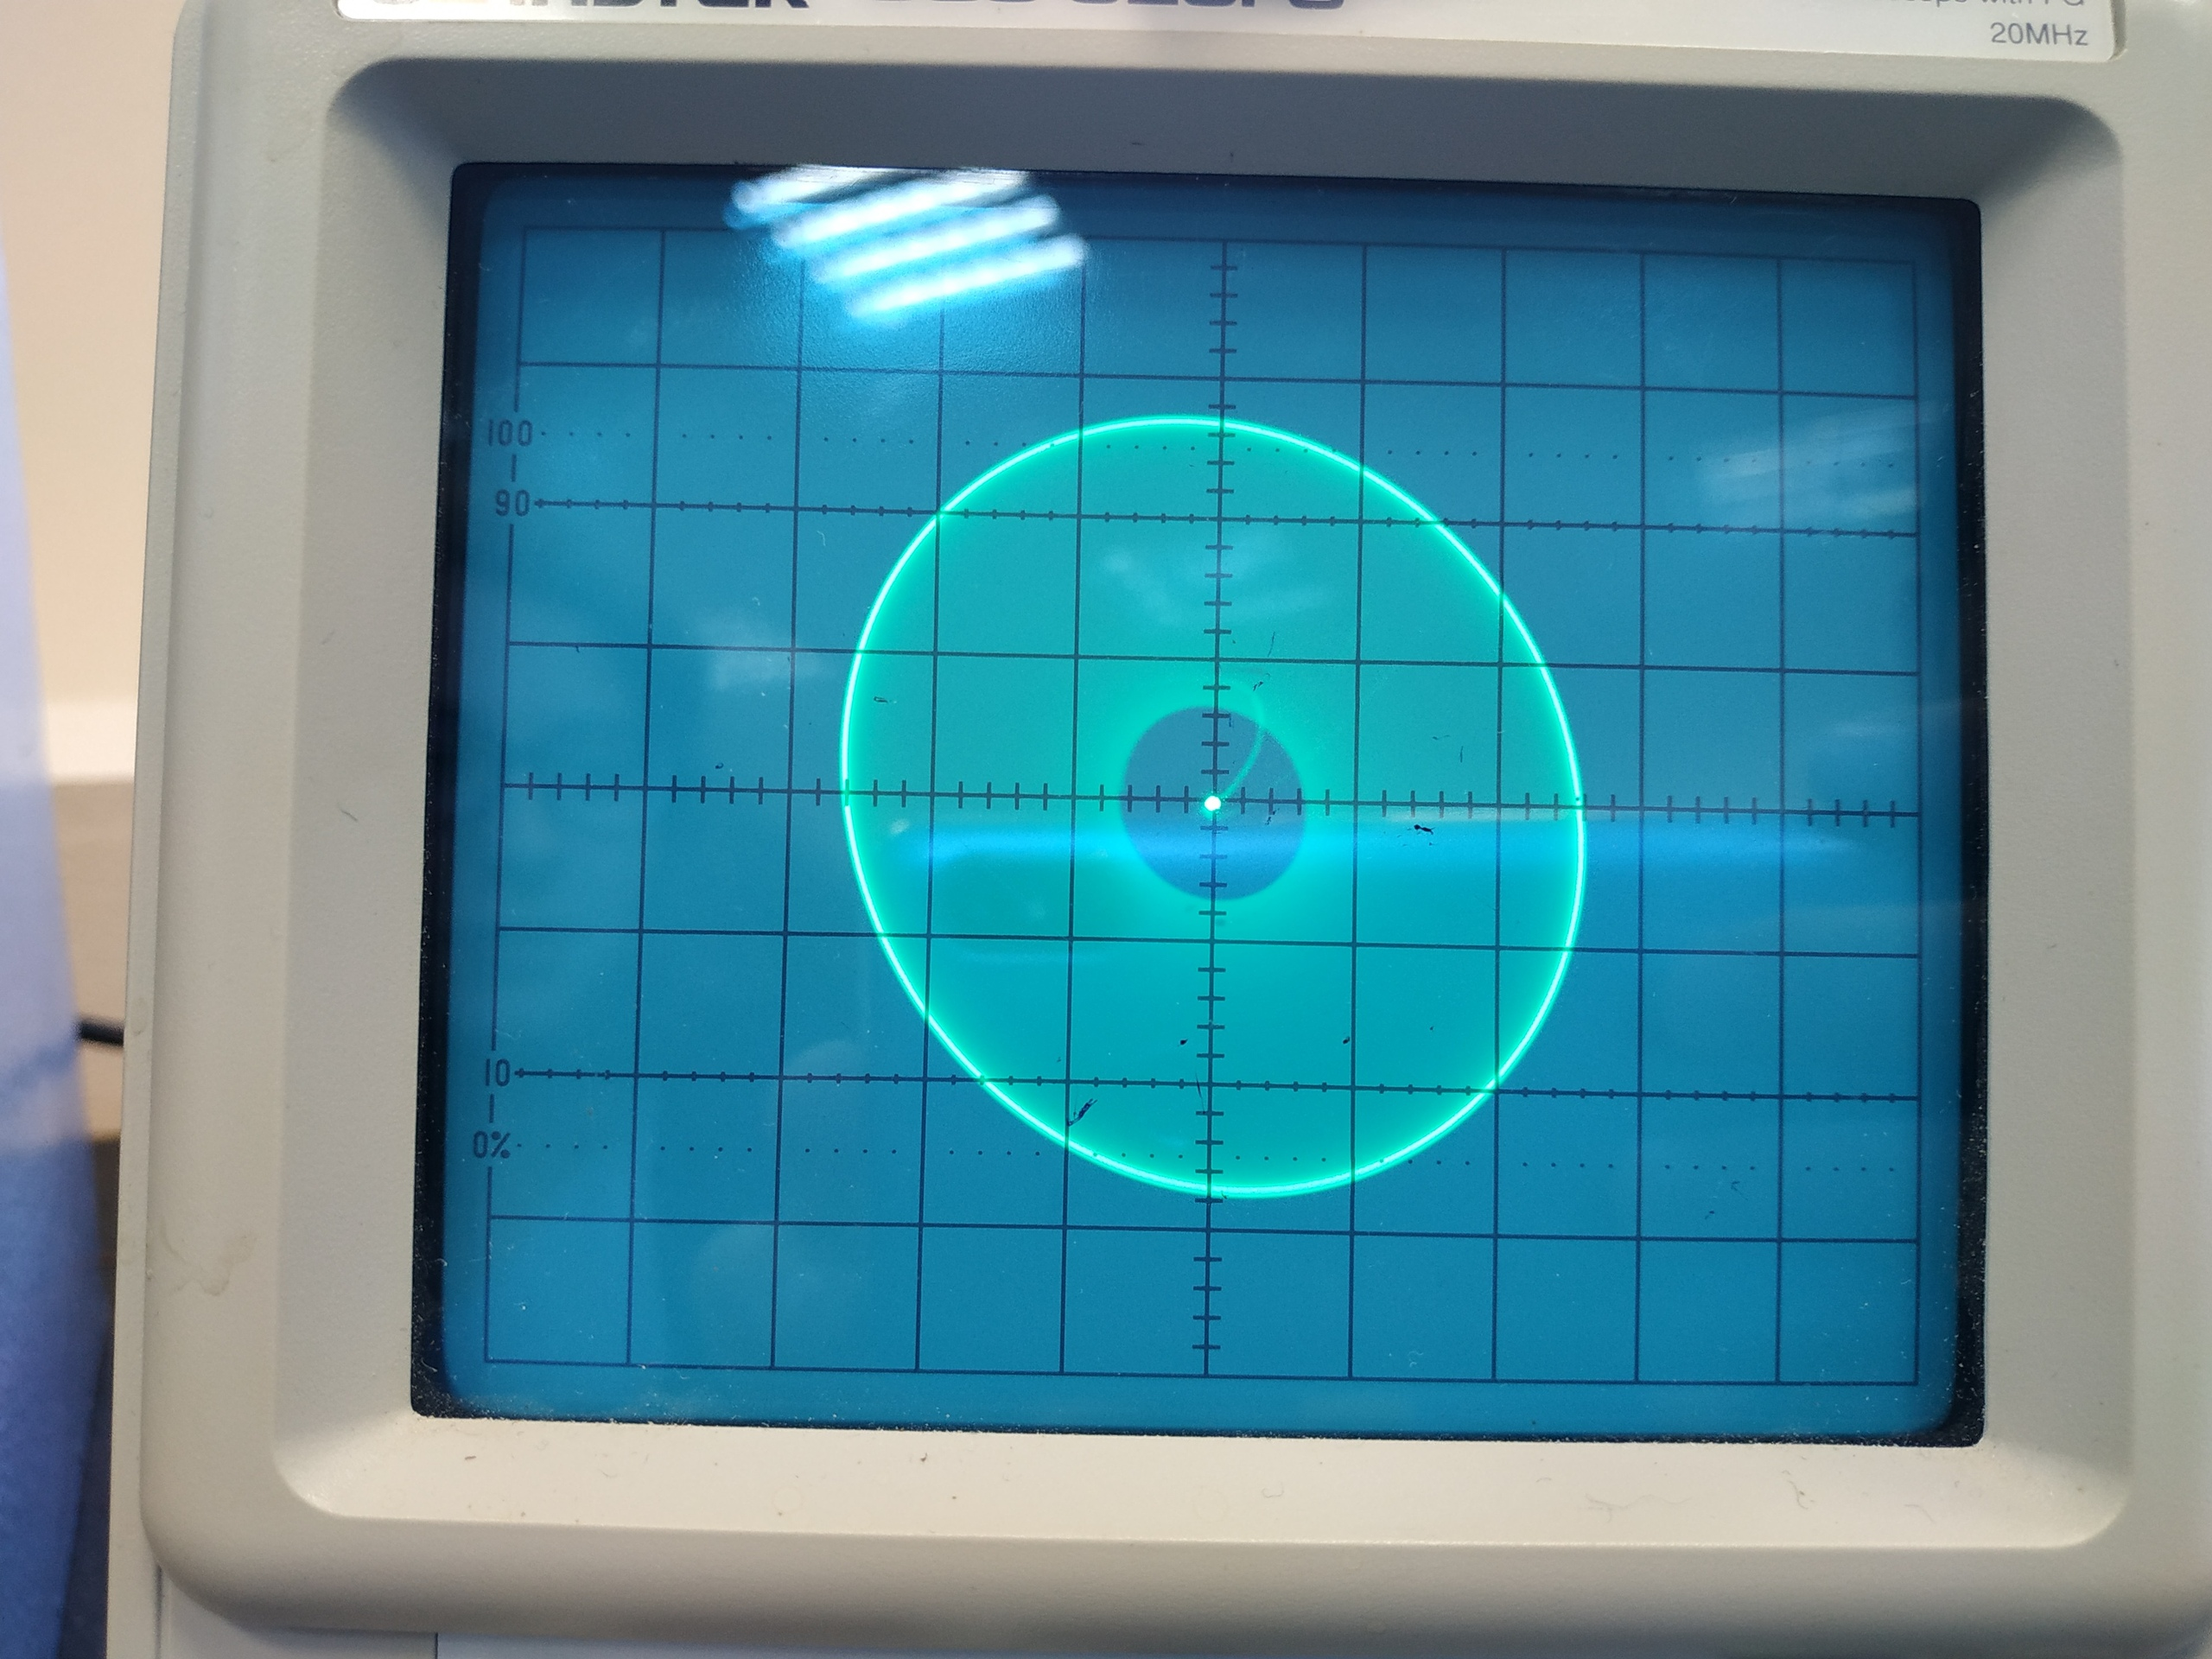
\includegraphics[height=100pt]{img/20.jpg} 
%             \vspace{0pt}
%             \label{fig:11}
%             \captionof{subfigure}{} 
%         \end{minipage}
%         \begin{minipage}{0.32\linewidth}
%             \centering
%             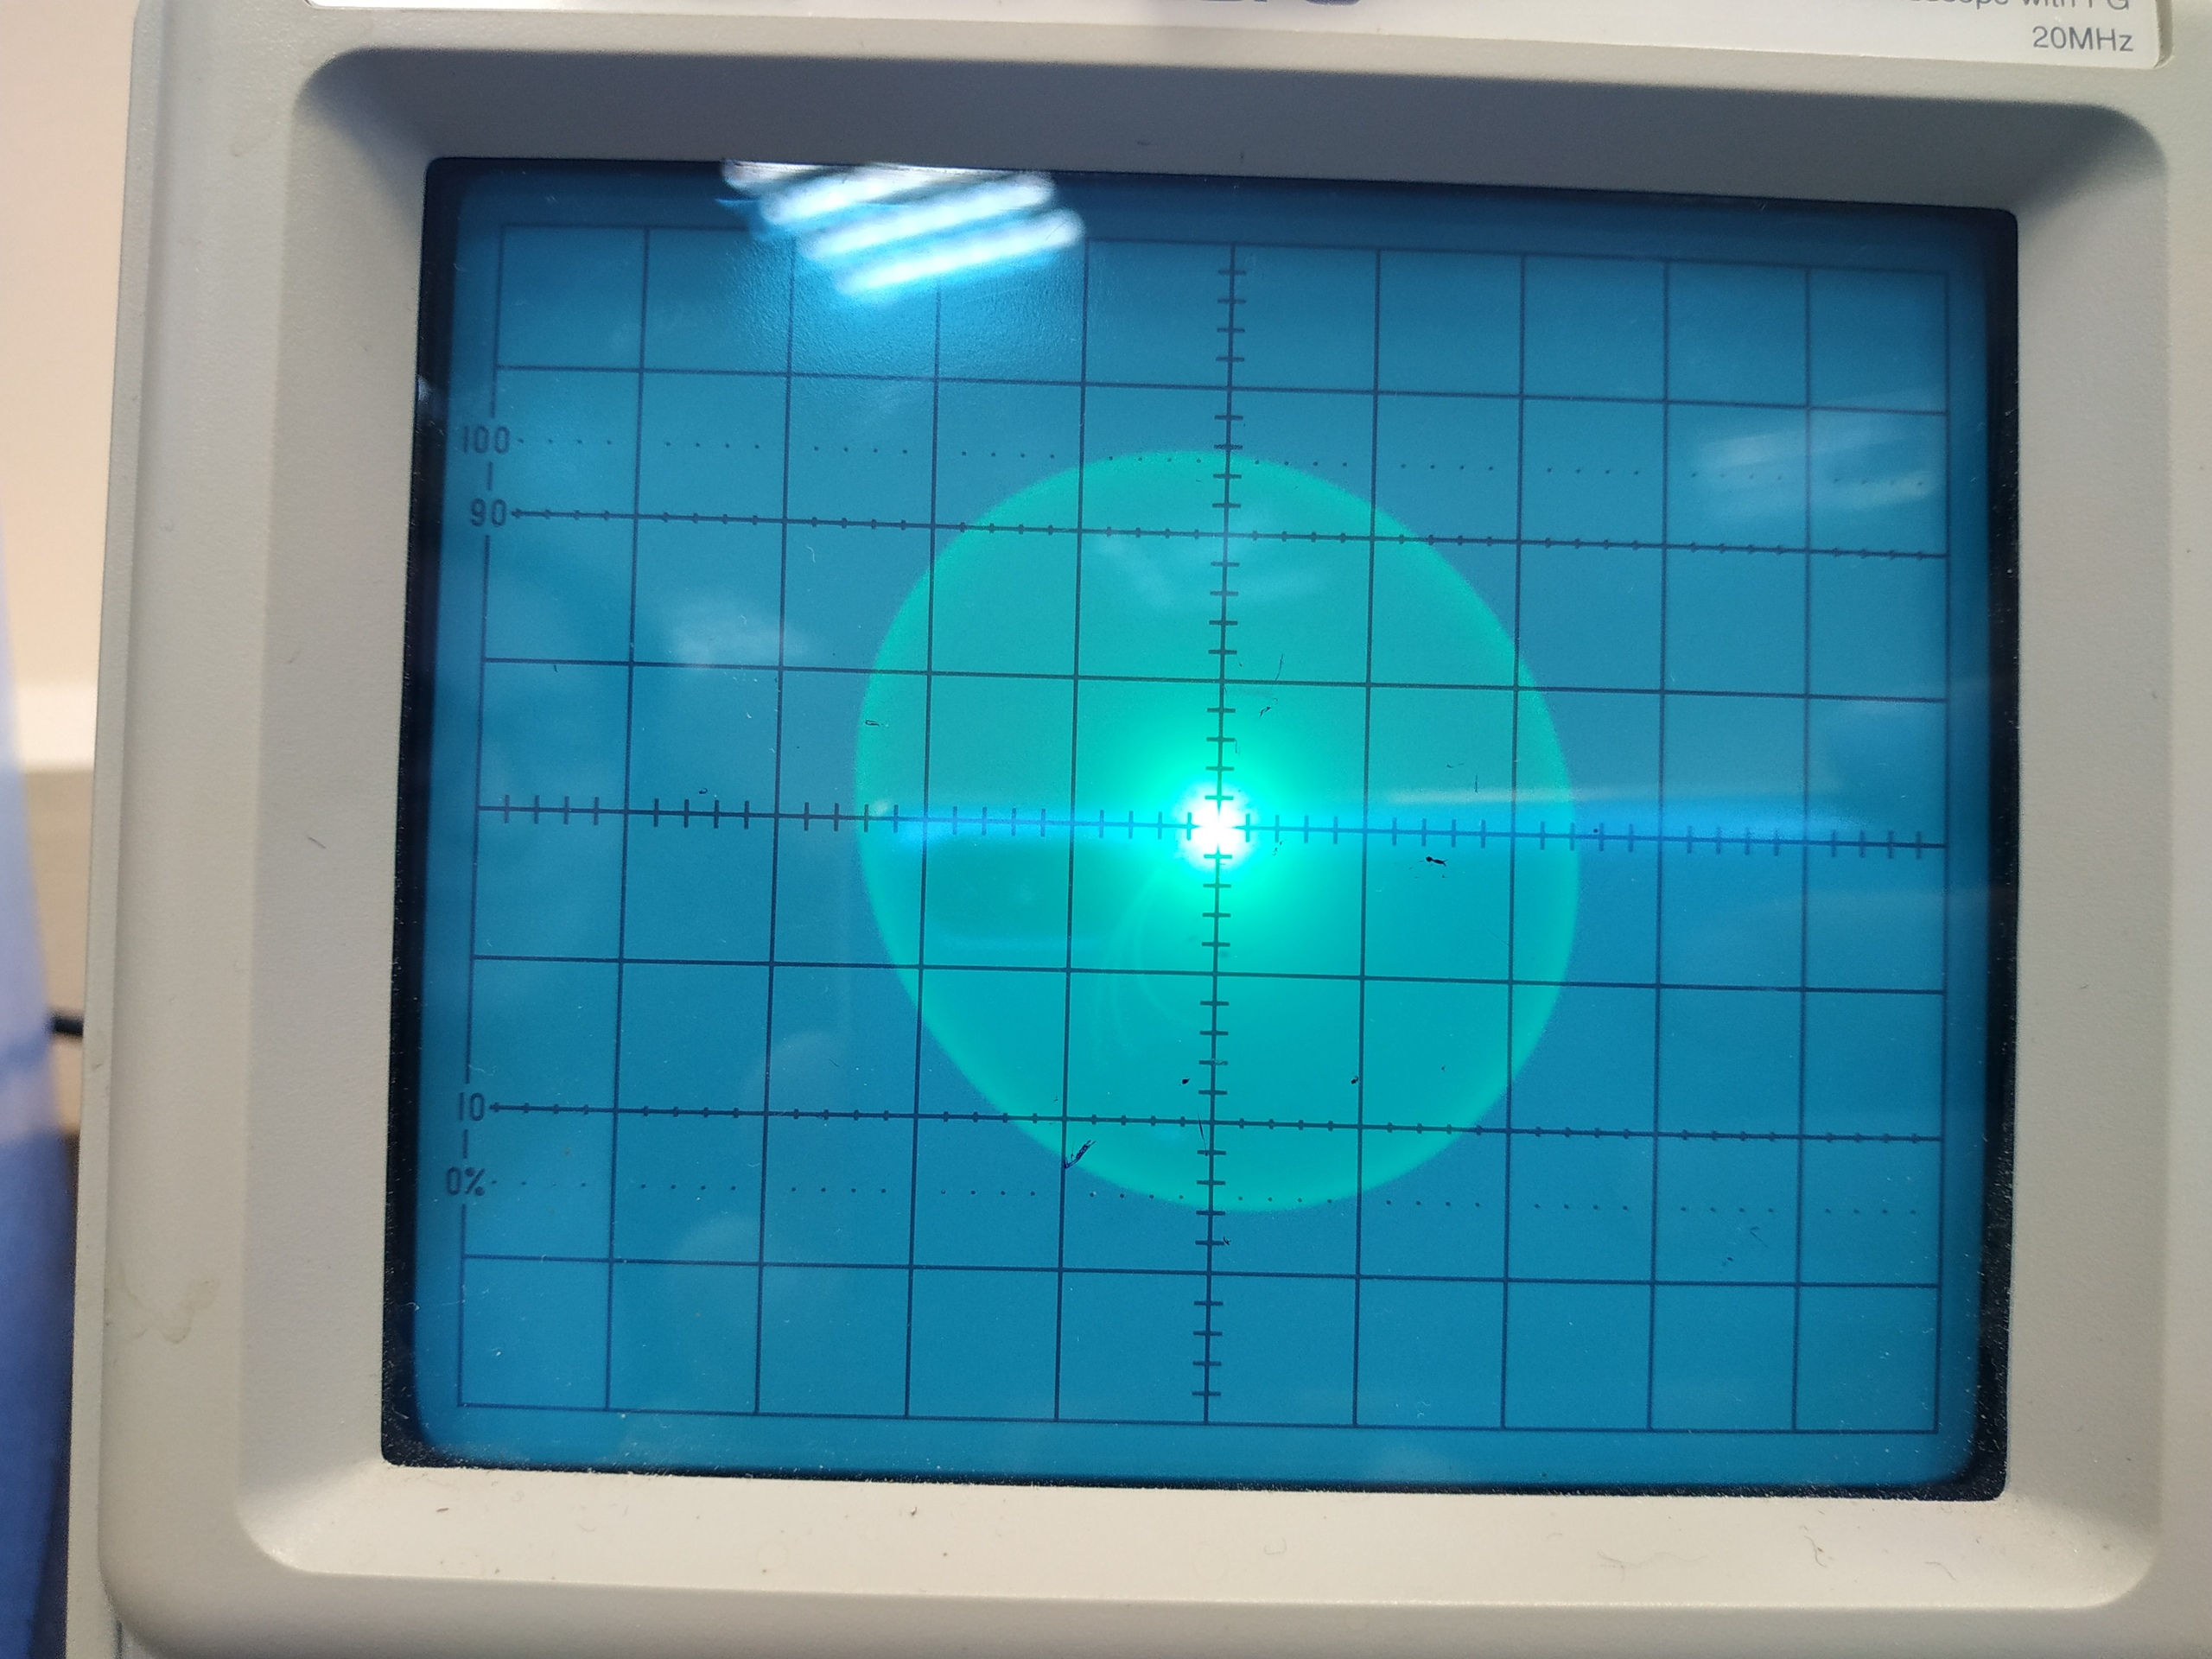
\includegraphics[height=100pt]{img/19.jpg} 
%             \vspace{0pt}
%             \label{fig:12}
%             \captionof{subfigure}{} 
%         \end{minipage}
%     \caption{Фазовая траектория для $M''< M $}
%     \vspace{-40pt}
%     \end{figure}
% \end{center} 



\section{Вывод}
В ходе работы были изучены три различных режима возбуждения лампового генератора, установлена зависимость амплитуды автоколебаний от параметров системы.
 Для каждого из режимов удалось получить бифуркационные диаграммы, которые по характеру поведения совпадают с теоретическими, а также фазовые траектории при 
 различных начальных условиях для разных параметров системы. Апериодический процесс для мягкого типа наблюдать не удалось. 

\end{document}

